\documentclass[diss]{mdtufsm}
%\documentclass[diss, twoside, openright]{mdtufsm} %- IMPRESSÃO (+ 100 PÁGINAS)

\usepackage[justification=justified]{caption}
\captionsetup{
	justification=raggedright,
	figurewithout,labelsep=endash,
	singlelinecheck=false
	}

\usepackage{minted}
\usepackage{chngcntr}
\counterwithout{figure}{chapter}
\counterwithout{table}{chapter}
\usepackage{ragged2e}
\usepackage{colortbl}
\usepackage{times}
\usepackage{setspace}
\usepackage{array,multirow}
\usepackage{float} 
\usepackage[portuguese,titlenumbered,ruled,linesnumbered]{algorithm2e}
\usepackage[T1]{fontenc}
\usepackage{fix-cm}
\usepackage{times, color, xcolor}
\usepackage[utf8]{inputenc}
\usepackage{graphicx}
\usepackage{amsmath,latexsym,amssymb}
%%%%%%%%%%%%%%%%%%%%%%%%%%%%%%%%%%%%%%%%%%%%%%%%%%%%%%%%%%%%%%%%%%%%%%
%%%%%%%%%%%%%%%%%%%%%%%%%%%%%%%%%%%%%%%%%%%%%%%%%%%%%%%%%%%%%%%%%%%%%%
%%%%%%%%%%%%%%%%%%%%%%%%%%%%%%%%%%%%%%%%%%%%%%%%%%%%%%%%%%%%%%%%%%%%%%
%%%%%%%%%%%%%%%%%%%%%%%%%%%% EDITAR %%%%%%%%%%%%%%%%%%%%%%%%%%%%%%%%%%
\usepackage[%hidelinks%, 
            bookmarksopen=true,linktocpage,colorlinks=true,
            linkcolor=black,citecolor=black,filecolor=magenta,urlcolor=blue,
            pdftitle={Gerenciamento Dinâmico de Memória em Aplicações com Reuso de Dados no Apache Spark},
            pdfsubject={Dissertação de Mestrado},
            pdfkeywords={Memória, LRU, Dinâmico, Apache, Spark,}
            ]{hyperref} 

%%%%%%%%%%%%%%%%%%%%%%%%%%%%%%%%%%%%%%%%%%%%%%%%%%%%%%%%%%%%%%%%%%%%%%
%%%%%%%%%%%%%%%%%%%%%%%%%%%%%%%%%%%%%%%%%%%%%%%%%%%%%%%%%%%%%%%%%%%%%%
%%%%%%%%%%%%%%%%%%%%%%%%%%%%%%%%%%%%%%%%%%%%%%%%%%%%%%%%%%%%%%%%%%%%%%

\usepackage[inner=30mm,outer=20mm,top=30mm,bottom=20mm]{geometry} 
\usepackage{multirow}
\usepackage{adjustbox}
\usepackage{mathtools}
\usepackage{verbatim}
\usepackage{array}
\usepackage{listings}
\usepackage{minted}

\usepackage{pifont}
\newcommand{\cmark}{\ding{51}}%
\newcommand{\xmark}{\ding{55}}%
\newcommand{\smark}{\ding{83}}


\usepackage{fancybox}
\makeatletter
\newenvironment{CenteredBox}{% 
\begin{Sbox}}{% Save the content in a box
\end{Sbox}\centerline{\parbox{\wd\@Sbox}{\TheSbox}}}% And output it centered
\makeatother

\usepackage{pgfplots}
\usepackage{multicol}

\usetikzlibrary{patterns}




%%=============================================================================
%% Trampa para corrigir o bug do hyperref que redefine o caption das figuras e das
%% tabelas, n�o colocando o nome ``Figura'' antes do n�mero do mesmo na lista
%%=============================================================================

\makeatletter

\long\def\@caption#1[#2]#3{%
  \expandafter\ifx\csname if@capstart\expandafter\endcsname
                  \csname iftrue\endcsname
    \global\let\@currentHref\hc@currentHref
  \else
    \hyper@makecurrent{\@captype}%
  \fi
  \@ifundefined{NR@gettitle}{%
    \def\@currentlabelname{#2}%
  }{%
    \NR@gettitle{#2}%
  }%
  \par\addcontentsline{\csname ext@#1\endcsname}{#1}{%
    \protect\numberline{\csname fnum@#1\endcsname ~-- }{\ignorespaces #2}%
  }%
  \begingroup
    \@parboxrestore
    \if@minipage
      \@setminipage
    \fi
    \normalsize
    \expandafter\ifx\csname if@capstart\expandafter\endcsname
                    \csname iftrue\endcsname
      \global\@capstartfalse
      \@makecaption{\csname fnum@#1\endcsname}{\ignorespaces#3}%
    \else
      \@makecaption{\csname fnum@#1\endcsname}{%
        \ignorespaces
        \ifHy@nesting
          \expandafter\hyper@@anchor\expandafter{\@currentHref}{#3}%
        \else
          \Hy@raisedlink{%
            \expandafter\hyper@@anchor\expandafter{%
              \@currentHref
            }{\relax}%
          }%
          #3%
        \fi
      }%
    \fi
    \par
  \endgroup
}

\makeatother

%========================================
% Identificação do trabalho
%========================================

\title{Gerenciamento Dinâmico de Memória em Aplicações com Reuso de Dados no Apache Spark}

\author{Donato}{Maurício Matter}
%\autoratrue

\titulacao{Mestre}

\course{Pós-Graduação em Ciência da Computação }
\initials{PPGCC} 
\institute{Centro de Tecnologia}
\degree{Mestre em Ciência da Computação}

% Para mestrado deixar sem opção dentro do {}
\trabalhoNumero{}

\advisoronepage[Prof.]{Dra.}{Barcelos}{Patrícia Pitthan de Araújo}
\advisor[Prof.]{Dra. (UFSM)}{Barcelos}{Patrícia Pitthan de Araújo}
\orientadoratrue
\committee[Dr.]{Lima}{João Vicente Ferreira}{UFSM}
\committee[Dr.]{Wives}{Leandro Krug}{UFRGS}

\date{25}{Maio}{2020} 

\keyword{Spark}
\keyword{Gerenciamento} 
\keyword{Memória}
\keyword{Reuso}
\keyword{Dinâmico}

\keywordAbstract{Spark}
\keywordAbstract{Management}
\keywordAbstract{Memory}
\keywordAbstract{Reuse}
\keywordAbstract{Dynamic}

%========================================
%% Início do documento
%========================================
\begin{document}
	
%========================================
%% Capa e folha de rosto
%========================================
\maketitle

%========================================
%% Catalogação (obrigatório para mestrado) e Folha de aprovação
%========================================
\newgeometry{inner=20mm,outer=30mm,top=30mm,bottom=20mm}	
\makeCIP{mdonato@inf.ufsm.br} %email do autor		
\restoregeometry

\includeCIP{folhaAprovacao.pdf}

%========================================
%folha de aprovação
%========================================
% \makeapprove

%========================================
%% Dedicatória (opcional)
%========================================
% \chapter*{Dedicatória}


\vfill

\begin{center}
	
	{\sffamily\itshape Dedico este trabalho aos meus pais Celso Garcia e Nadir Garcia; a minha companheira de todas as horas Luísa Lucca; aos irmãos que a vida me deu Maurício Schneider e Guilherme Gaiardo; aos amigos, familiares e mestres.}
	
\end{center}

\vfill

\newpage

%========================================
%% Agradecimentos (opcional)
%========================================
% \chapter*{Agradecimentos}


\justifying{\textit{Aos meus pais, \textbf{Nadir Garcia} e \textbf{Celso Garcia}, pelo amor, carinho e incentivo incondicional. Vocês foram, são e sempre serão meus maiores exemplos de vida.}}

\justifying{\textit{A minha companheira, amor e melhor amiga \textbf{Luísa Lucca} por estar ao meu lado durante toda esta etapa, sempre solícita e carinhosa, presente tanto nos momentos difíceis quanto nas comemorações de cada conquista alcançada.}}

\justifying{\textit{Aos amigos \textbf{Maurício Schneider} e \textbf{Guilherme Gaiardo}, considerados por mim como grandes irmãos, que sempre estiveram próximos nas etapas mais importantes da minha vida, passando boas energias e torcendo pelo meu sucesso.}}

\justifying{\textit{Aos demais \textbf{amigos} que, seja em Santo Ângelo, em Santa Maria ou em qualquer outro lugar do mundo, me possibilitaram viver ótimos momentos. Ainda, gostaria de agradecer em especial aos colegas \textbf{Matheus Garay}, \textbf{Thales Tavares}, \textbf{Leonardo Marcuzzo}, \textbf{Maurício Donato} e \textbf{Brenda Salenave} que, pessoalmente ou virtualmente, estiveram presentes no meu dia a dia nesses últimos dois anos.}}

\justifying{\textit{Ao laboratório \textbf{GRECA} que me acolheu de braços abertos durante todo o período do mestrado. Nesse mesmo, tive a oportunidade e o privilégio de trabalhar e compartilhar experiências com excelentes colegas, em especial com meus veteranos e amigos \textbf{Nilton Camargo} e \textbf{Anderson Monteiro}.}}

\justifying{\textit{Ao grupo de trabalho \textbf{FENDE} que participou ativamente da minha formação, me permitindo conhecer e cooperar com pesquisadores de extrema competência e saber.}}

\justifying{\textit{Finalmente, a todos os \textbf{professores} que dividiram seus conhecimentos comigo. Principalmente, ao professor \textbf{Carlos Raniery} que não apenas me orientou durante a elaboração deste trabalho, mas também na realização de projetos e decisões que o antecederam e que o sucederão. Também, não posso deixar de lembrar do professor \textbf{Sérgio Mergen}, cooperativo e incentivador desde meados da minha graduação.}}

\justifying{\textit{Todos os aqui citados ocupam um lugar especial no meu coração, sem vocês nenhuma conquista teria real sentido. Desejo a todos muito sucesso e deixo aqui o meu mais profundo e significativo \textbf{ORBRIGADO}!!}}

%========================================
%% Epígrafe (opcional)
%========================================
% \clearpage
\begin{flushright}
\mbox{}\vfill

{\sffamily\itshape
	\begin{quote}
		\begin{quote}
			\begin{quotation}
			"We can only see a short distance ahead, but we can see plenty there that needs to be done."\\
			
			\begin{flushright}
			\textsc{(Alan Turing)}
		  	\end{flushright}
		  	
		\end{quotation}
		\end{quote}
	\end{quote}
 }




\end{flushright}


%========================================
%% Resumo
%========================================
\begin{abstract}
\begin{justify}
O Apache Spark é um \textit{framework} capaz de processar grandes quantidades de dados em memória, através da sua principal abstração: o \textit{Resilient Distributed Datasets} (RDD). Um RDD consiste em uma coleção imutável de objetos, os quais podem ser operados de maneira paralela e distribuída no\textit{cluster}. Uma vez processados, RDDs podem ser mantidos em \textit{cache}, possibilitando a sua reutilização sem realizar a sua recomputação. Conforme a computação da aplicação é feita, a memória tende a ficar sobrecarregada e, portanto, partições de RDDs devem ser removidas de acordo com o algoritmo \textit{Least Recently Used} (LRU). Este algoritmo é baseado na observação de que partições frequentemente utilizadas em um passado recente tendem a ser acessadas novamente em um futuro próximo. Deste modo, remove-se a partição cujo acesso ocorreu há mais tempo. Entretanto, há situações em que o LRU pode acarretar em uma degradação no desempenho, como é o caso onde há acessos cíclicos à memória e a quantidade de dados manipulados é maior que o espaço disponível. Nessas situações,o LRU sempre irá remover um bloco que será acessado em um futuro próximo. Considerando tal problemática, este trabalho propõe um modelo de Gerenciamento Dinâmico da Memória em Aplicações com Reuso de Dados no Apache Spark. Este modelo busca extrair métricas da aplicação em execução a fim de utilizar estas informações para realizar remoção dos dados em \textit{cache}. O modelo proposto é composto por dois componentes principais, sendo estes (1) um algoritmo de gerenciamento das partições de RDDs armazenadas em memória e (2) um agente de monitoramento responsável por obter informações sobre a execução de aplicações. O modelo de Gerenciamento Dinâmico foi validado através da realização de experimentos utilizando a plataforma Grid’5000 com os \textit{benchmarks PageRank}, \textit{K-Means} e \textit{Logistic Regression}. Os resultados obtidos demonstram que o modelo de Gerênciamento Dinâmico conseguiu realizar um melhor aproveitamento da memória disponível, chegando a reduzir em 23,94\% o tempo médio necessário para processar o \textit{benchmark Logistic Regression}, quanto comparado ao LRU. Ademais, o modelo proposto tornou a execução do Spark mais estável, reduzindo a frequência de erros no processamento dos \textit{benchmarks}. Como consequência, houve uma redução de até 34,15\% no tempo de execução do \textit{benchmark PageRank}. Portanto, estes resultados permitem concluir que estratégias dinâmicas, como a proposta por este estudo, podem proporcionar um ganho no desempenho do Spark no processamento de aplicações onde existe o reuso de dados.

\end{justify} 
\end{abstract}

%========================================
%% Abstract
%========================================
\begin{englishabstract}
{Dynamic Memory Management in Applications With Data Reuse on Apache Spark}
%%============ MANTER ESSA LINHA ============================================
\ %%============ MANTER ESSA LINHA ==========================================
%%============ MANTER ESSA LINHA ============================================
\ %%============ MANTER ESSA LINHA ==========================================
%%============ MANTER ESSA LINHA ============================================
\ %%============ MANTER ESSA LINHA e deixar uma em branco ===================

\begin{justify}
The Apache Spark is a framework able to process a massive quantity of data in-memory, through its primary abstraction: Resilient Distributed Datasets (RDD). An RDD consists of an immutable object collection, which can be processed in a parallel and distributed way in the cluster. Once it was processed, an RDD could be stored in the cache, allowing its reuse without recomputing it. While the application's computations are done, the memory tends to be overheaded, and RDD's partitions must be removed according to the Least Recently Used (LRU) algorithm. This algorithm is based on the idea that partitions frequently used in the past will be reaccessed shortly. Thus, the algorithm removes partitions that access occurred a long time ago. However, there are situations that the LRU algorithm could introduce degradation in Spark's performance, which is the case where there is cyclic access in the memory, and the available space is lower than the dataset size. In those situations, the LRU algorithm will always remove the block, which will be accessed soon. Considering the identified issues in the LRU, this work proposes a Dynamic Memory Management in Applications With Data Reuse on Apache Spark. This model aims to extract metrics from the application's execution in order to use that information to realize data removing from the cache. The proposed model is compound by two main components, which are (1) an algorithm to manage the RDD's partitions stored int the memory and (2) a monitor agency responsible for getting information about the application. The Dynamic Management model was validated through experiments using the Grid'5000 platforms with benchmarks PageRank, K-Means, and Logistic Regression. The obtained results demonstrate that the Dynamic Management model was able to improve the utilization of available memory, being able to reduce by 23,94\% the necessary execution time to process the benchmark Logistic Regression, when it is compared to LRU.
Furthermore, the proposed model became Spark's execution more stable, reducing the error frequency during the processing of benchmarks. As a consequence, there was a reduction by 34,14\% in the time spend to process the benchmark PageRank. Therefore, the obtained results allow concluding that dynamic strategies, like the one proposed by this work, can improve the Sparks execution in applications where there is reuse data.
\end{justify}
\end{englishabstract}

%========================================
%% Lista de figuras (comentar se não houver)
%========================================
\listoffigures

%========================================
%% Lista de tabelas (comentar se não houver)
%========================================
\listoftables

%========================================
%% Lista de Apêndices (comentar se não houver)
%========================================
%\listofappendix

%========================================
%% Lista de Anexos (comentar se não houver)
%========================================
%\listofannex

%========================================
%% Lista de abreviaturas e siglas
%========================================
 %o parametro deve ser a abreviatura mais longa
\begin{listofabbrv}{UbiComp}
      \item[API]    \textit{Application Program Interface} 
      \item[ASRW]   \textit{Actions Sequence and RDD Weight}
      \item[CPU]    \textit{Central Processor Unit} 
      \item[DAG]    \textit{Directed Acyclic Graph} 
      \item[GB]     \textit{GigaByte} 
      \item[GC]     \textit{Garbage Collector} 
      \item[HD]     \textit{Hard Drive}
      \item[HDFS]   \textit{Hadoop Distributed File System} 
      \item[IP]     \textit{Internet Protocol} 
      \item[JDK]    \textit{Java Development Kit}
      \item[JSON]   \textit{JavaScript Object Notation}
      \item[JVM]    \textit{Java Virtual Machine} 
      \item[LCS]    \textit{Low Cost Strategy} 
      \item[LRU]    \textit{Least Recently Used}
      \item[MB]     \textit{MegaByte}
      \item[RAM]    \textit{Random Access Memory} 
      \item[REST]   \textit{Representational State Transfer} 
      \item[RDD]    \textit{Resilient Distributed Datasets} 
      \item[RPC]    \textit{Remote Procedure Call} 
      \item[URL]    \textit{Uniform Resource Locator} 
\end{listofabbrv}

%========================================
%% Lista de simbolos (opcional)
%========================================
%Simbolos devem aparecer conforme a ordem em que aparecem no texto
% o parametro deve ser o símbolo mais longo
%\begin{listofsymbols}{teste}
%  \item [$\nu$] Símbolos Não Terminais (Nu)
%  \item [$\tau$] Símbolos Terminais (Tau)
%  \item [$\rho$] Regras de Produção (Rho)
%  \item [$\varsigma$] Símbolo Inicial (Sigma)
%\end{listofsymbols}

%========================================
%% Sumário
%========================================
\tableofcontents

%========================================
%% Início da dissertação
%========================================
\setlength{\baselineskip}{1.5\baselineskip}

\justifying
\chapter{Introdução}
Os avanços nas tecnologias de informação permitiram o armazenamento de grandes e variados conjuntos de dados. Com o advento da \textit{internet}, interações \textit{online} estão cada vez mais presentes no cotidiano, possibilitando a comunicação entre pessoas e empresas de maneira fácil e descomplicada. Como consequência dessa interatividade, a quantidade de dados tem crescido a uma taxa significativa durante os últimos anos \cite{goldschmidt2015data}. 

Os dados, os quais podem ir desde manifestações em redes sociais até movimentações financeiras, são gerados e disponibilizados em diferentes tamanhos e formatos. De acordo com \cite{mcafee2012big}, através desses dados, gerentes podem medir e entender seus negócios e, consequentemente, traduzir esse conhecimento em decisões melhores. 
Porém, a realização das etapas necessárias para extrair conhecimento a partir dos dados implica em altos custos econômicos e computacionais, uma vez que o armazenamento e o processamento dos mesmos não são tarefas triviais. Para \cite{oussous2018big}, essas dificuldades afetam a captura, o armazenamento, a pesquisa, o compartilhamento, a análise, a gerência e a visualização desses dados. Além disso, a segurança e a privacidade são problemas em aplicações orientadas a dados. 

O processamento desses dados requer, por muitas vezes, ferramentas capazes de recorrer ao processamento paralelo e distribuído entre um conjunto de máquinas (\textit{cluster}), além de suportar altas variações no volume de dados utilizado. \textit{Frameworks} baseados no paradigma \textit{MapReduce}, como o Apache Hadoop, têm sido amplamente utilizados para o processamento de grandes volumes de dados. De forma geral, esses \textit{frameworks} oferecem operações de processamento de alto nível e abstrações para acesso aos recursos do \textit{cluster} com o objetivo de facilitar o desenvolvimento de aplicações pelos usuários. 

Entretanto, os \textit{frameworks} baseados no paradigma \textit{MapReduce} falham em oferecer abstrações para acesso à memória distribuída tornando-os ineficientes no processamento de algoritmos de reutilização, como aqueles utilizados em Mineração de Dados e Aprendizado de Máquina, \cite{zaharia2012rdd}. Nesse sentido, o Apache Spark\footnote{Disponível em: https://spark.apache.org/} surge como um \textit{framework} capaz de processar grandes quantidades de dados de maneira paralela e distribuída estendendo o modelo \textit{MapReduce}, já consolidado pelo Apache Hadoop, de modo a facilitar o desenvolvimento de aplicações com reutilização de dados. 

O Spark foi projetado para implementar um mecanismo de execução multiestágio em memória principal juntamente com sua principal abstração, o \textit{Resilient Distributed Datasets} ou simplesmente RDD \cite{zaharia2012rdd}). Dessa forma, o Spark consegue alcançar um desempenho superior quando comparado ao mecanismo baseado em disco utilizado pelo Hadoop. Este desempenho é obtido através da capacidade de processar diversas computações em memória, dispensando a escrita de dados intermediários em disco, diferentemente do Hadoop. Para tanto, o RDD visa encapsular a manipulação dos dados que serão processados pela aplicação, distribuindo-as através dos nodos do \textit{cluster} e assim permitindo a sua execução em memória.

Um RDD consiste em uma coleção imutável de objetos, os quais podem ser operados e processados de forma paralela e distribuída entre os nodos do \textit{cluster}. Uma vez realizado o processamento de um determinado RDD, este pode ser mantido em \textit{cache} para que seja possível reutilizá-lo em futuras computações sem necessidade de efetuar o seu reprocessamento, tornando a execução da aplicação mais eficiente. 

Conforme novos RDDs são armazenados e processados, a memória disponível tende a ficar esgotada e, portanto, políticas de gerenciamento de memória devem ser utilizadas. Assim, em situações de sobrecarga no uso do espaço disponível, o Spark remove partições mantidas em \textit{cache} de acordo com o algoritmo LRU (\textit{Least Recently Used}) \cite{luu2018beginning}, o qual remove partições cujo acesso ocorreu há mais tempo, explorando apenas a localidade temporal do acesso. Desta forma, é possível gerar situações onde apenas uma fração do RDD permanece armazenado em \textit{cache}. 

Entretanto, cabe ao desenvolvedor da aplicação Spark identificar e selecionar os RDDs que deverão ser mantidos em \textit{cache}. De acordo com \cite{zecevic2016spark}, é importante manter os dados em \textit{cache} para algoritmos iterativos, uma vez que esses tendem a reutilizar os dados.  Por padrão, os dados são armazenados em memória principal, uma vez que esta possui uma menor latência para acesso aos dados quando comparado ao armazenamento estável. Entretanto, é possível utilizar o armazenamento estável ou uma combinação deste juntamente com a memória principal.

\section{Justificativa}
Através do RDD, o Spark permite a realização de diversas computações em memória principal a fim de evitar a escrita de resultados intermediários no armazenamento estável. Ainda, RDDs podem ser mantidos em \textit{cache}, possibilitando a sua reutilização na aplicação sem realizar a sua recomputação. Conforme realiza-se a computação dos RDDs da aplicação, a memória tende a ficar sobrecarregada e, portanto, partições devem ser removidas de acordo com o algoritmo LRU.

O LRU é um algoritmo clássico para o gerenciamento de memória, sendo empregado nos mais variados sistemas \cite{robinson1990data}. Este algoritmo é baseado na observação de que partições frequentemente utilizadas em um passado recente tendem a ser acessadas novamente em um futuro próximo. Deste modo, a partição removida da memória é aquela cujo acesso ocorreu há mais tempo, uma vez que esta apresenta a menor chance de ser acessada novamente em um futuro próximo.

Embora o LRU seja de fácil implementação \cite{kim2000low} e apresente bons resultados, há situações onde existe degradação no desempenho. Um exemplo do comportamento indesejado desse algoritmo ocorre quando há acessos cíclicos à memória, como em um \textit{loop}, em que a quantidade de dados manipulados é maior que o espaço disponível em \textit{cache}. Nessas situações,o LRU sempre irá remover um bloco que será acessado em um futuro próximo, uma vez que estes são os blocos acessados há mais tempo \cite{jiang2002lirs}. Deste modo, considera-se apenas o tempo desde o último acesso ao bloco de memória, ignorando a sua necessidade em um futuro bem próximo.

Dentre as classes de problemas abordadas pelo Spark, um dos grandes focos é o processamento de aplicações onde há reutilização de dados em iterações futuras. Especificamente nesta classe de aplicações, o comportamento do acesso aos dados pode ser semelhante ao acesso cíclico à memória, evidenciando um dos problemas da utilização do LRU neste tipo de aplicação. Consequentemente, a utilização deste algoritmo pelo Spark para o gerenciamento da memória pode acarretar em degradação no desempenho do \textit{framework}.

\section{Objetivos do Trabalho}
Buscando alcançar um desempenho superior no processamento de aplicações com reutilização de dados, este trabalho tem como objetivo o desenvolvimento de um modelo de Gerenciamento Dinâmico da Memória no Spark. Por meio deste modelo, busca-se extrair métricas da execução da aplicação e dos RDDs utilizados por esta, de modo a utilizar estas informações para realizar remoção dos dados em \textit{cache}, bem como decidir o momento em que essas operações devem ser executadas.

Para tanto, o modelo de Gerenciamento proposto é dividido em dois componentes: um algoritmo de gerenciamento das partições de RDDs armazenadas em memória e um agente de monitoramento responsável por obter informações sobre a execução de aplicações.

O algoritmo utilizado para realizar o gerenciamento da memória implementada por este modelo visa decidir quais blocos devem ser removidos da memória em situações onde a mesma encontra-se sobrecarregada. Tal implementação é baseada no algoritmo LRU e consiste em combinar a frequência de reutilização, extraída a partir dos RDDs identificados na aplicação, com a localidade temporal proporcionada pelo LRU.

O agente de monitoramento tem como objetivo prever a necessidade de remoção de partições da memória, por meio da instrumentação da execução de aplicações Spark. Este agente consiste em uma aplicação Java, responsável por acompanhar o andamento da execução da aplicação e a quantidade de memória utilizada para realizar o processamento da aplicação em questão.

A previsão da necessidade de liberar espaço em memória é realizada utilizando dois critérios: um \textit{threshold} de ocupação da memória e o estado atual da execução da aplicação. O limiar de ocupação busca definir um limite máximo para a quantidade de memória ocupada, sendo inferior a 100\%, de modo a garantir que haja  espaço disponível para novos dados. O estado atual da execução da aplicação refere-se a quantidade de memória utilizada pela aplicação e a existência de computações pendentes para execução.

Assim, cenários onde a memória ocupada é superior ao \textit{threshold} e ainda há computações pendentes indicam a possível necessidade de liberação de espaço na memória. Uma vez identificada esta necessidade, o agente de monitoramento envia uma notificação ao nodo Spark cuja memória encontra-se sobrecarregada, para que este nodo execute a remoção de partições da memória. Esta notificação é feita através do Apache ZooKeeper.

A validação do modelo para Gerenciamento Dinâmico da Memória é realizada por meio de experimentos, visando avaliar o tempo de execução dos \textit{benchmarks}, visto que o tempo utilizado para processar as aplicações apresenta o maior impacto quando alterada a política de gerenciamento de memória. Através desta avaliação, compara-se o modelo proposta ao algoritmo LRU implementado nativamente pelo Spark em versões 2.x, uma vez que estas versões apresentam diferenças no gerenciamento da memória utilizada. 

Os experimentos foram realizados com \textit{benchmarks} focados na reutilização de dados em computações futuras. Para isto, utilizou-se as aplicações \textit{PageRank}, \textit{Logistic Regression} e \textit{K-Means}, visto que cada aplicação apresenta um comportamento diferente durante sua execução. 

\section{Estrutura do Trabalho}
O restante do trabalho encontra-se organizado da seguinte maneira: no Capítulo \ref{cap:referencial-teorico} são descritos os conceitos fundamentais acerca das ferramentas utilizadas no desenvolvimento do trabalho. Além disso, neste Capítulo é apresentado e discutido os trabalhos relacionados a este, encontrados na literatura. 

O Capítulo \ref{cap:implementacoes} é destinado a descrever o modelo de Gerenciamento Dinâmico proposto por este trabalho. Para tanto, é demonstrando o desenvolvimento do trabalho juntamente com os detalhes de funcionamento e implementação, bem como o processo de experimentação e os resultados obtidos. Por fim, o Capítulo \ref{cap:consideracoes-finais} apresenta as considerações deste trabalho.

\chapter{Referencial Teórico} \label{cap:referencial-teorico}
Este Capítulo apresenta a fundamentação teórica relativa a este trabalho. Para tanto, o Capítulo encontra-se organizado da seguinte maneira: na Seção \ref{sec:spark} é explicado o \textit{framework} Apache Spark juntamente com o modelo de memória utilizado. A Seção \ref{sec:Zookeeper} é dedicada à apresentação do Apache ZooKeeper. Por fim, a Seção \ref{sec:trab-relacionados} tem como objetivo explanar trabalhos relacionados a este, encontrados na literatura.

\section{Apache Spark}\label{sec:spark}
O Spark é um \textit{framework} de código aberto, projetado com o objetivo de realizar o processamento de dados massivos de maneira paralela e distribuída. A criação de aplicações Spark é realizada através de uma API (\textit{Application Program Interface}) disponibilidada pelo \textit{framework}. 

Através desta API, é possível criar e manipular RDDs \cite{karau2015learning}, utilizando transformações e ações. As transformações são métodos que recebem um RDD como entrada e geram um ou mais RDDs como saída. São exemplos de transformações os métodos \textit{map} e \textit{filter}. Enquanto o método \textit{map} aplica uma mesma função para todos os dados do \textit{dataset} contido no RDD, o método \textit{filter} realiza um filtro neste conjunto de dados, obedecendo uma condição definida pelo desenvolvedor. 

As ações são operações cujo objetivo é computar o RDD e gerar um valor, como é caso dos métodos \textit{reduce} e \textit{count}. O método \textit{reduce} agrega o conjunto de dados do RDDs em um único valor. Já o método \textit{count} realiza uma contagem do número de registros armazenados no RDD.

Juntamente com os métodos de transformações e ações, são disponibilizados ao desenvolvedor métodos auxiliares a fim de realizar o armazenamento de RDDs, permitindo que estes sejam mantidos em \textit{cache} após sua computação. A possibilidade de realizar a persistência dos dados evita que o RDD seja recomputado a cada reutilização em computações futuras. Neste sentido, dois métodos podem ser utilizados: \textit{cache()} e \textit{persist()}. O método \textit{cache()} armazena os dados em memória principal, sendo este o nível padrão para armazenamento dos dados em \textit{cache}. Por outro lado, o método \textit{persist()} permite que seja especificado o nível de armazenamento, isto é, memória, disco ou combinação de ambos, para manter as partições em \textit{cache}.

Internamente, um RDD é composto por:
\begin{itemize}
    \item[a)] uma lista de partições responsáveis por armazenar os dados. Geralmente, uma partição do RDD corresponde a um bloco de dado armazenado no HDFS (\textit{Hadoop Distributed File System)}, com tamanho padrão de até 128 MB para o Hadoop (versão 2);
    \item[b)] uma função para computar cada partição;
    \item[b)] uma lista de dependência de outros RDDs;
    \item[b)] opcionalmente, um particionador para RDDs chave-valor (isto é, hash-particionado) e;
    \item[b)] uma lista de locais preferidos no \textit{Cluster} para realizar a computação de cada partição, sendo este atributo opcional.
\end{itemize}

A avaliação dos RDDs criados é realizada de forma \textit{lazy}, ou seja, sua computação não é efetuada no momento de sua criação, sendo processados apenas quando for necessário. Quando um novo RDD é gerado, este carrega consigo uma referência do(s) RDD(s) ancestral(is), adicionado(s) a sua lista de dependências. Tal processo é realizado na criação de qualquer RDD, gerando o grafo direcionado acíclico de dependências da aplicação.

O grafo direcionado acíclico (DAG -- \textit{Directed Acyclic Graph}), denominado de \textit{lineage} do RDD, é utilizado para realizar a computação do RDD juntamente com suas respectivas dependências. Este grafo constitui um importante mecanismo de recuperação de falhas implementado pelo Spark. Assim, em situações onde partições são perdidas, o sistema pode realizar a recomputação dos dados a partir de uma réplica restante dos dados de entrada \cite{karau2015learning}.

Ao ser aplicada uma ação a um determinado RDD, este é submetido ao escalonador do Spark, denominado \textit{DAGScheduler}, com o objetivo de transformar a sua \textit{lineage} em um plano de execução físico composto por estágios. Para a criação destes estágios, o \textit{DAGScheduler} particiona o grafo do RDD em limites \textit{shuffle}, isto é, em limites onde há redistribuição dos dados entre partições. 

Dependências onde não há redistribuição de dados são enfileiradas em um mesmo estágio para serem computadas, como é o caso das transformações \textit{map} e \textit{filter}. Em contrapartida, dependências \textit{shuffle} requerem dois estágios para serem computadas, sendo o primeiro estágio para realizar a escrita dos arquivos de saída e um segundo estágio para ler estes dados, após uma barreira de sincronização entre as operações, \cite{DAGSchedulerSpark}. 

O procedimento de criação do plano de execução da aplicação, denominado de \textit{job}, é realizado sempre que uma ação é aplicada a um determinado RDD. Assim, a execução de uma mesma aplicação pode ser dividida em diversos \textit{jobs} até a sua completa finalização.

Após ser gerado o plano de execução físico pelo \textit{DAGScheduler}, o Spark executa os estágios da aplicação distribuindo o processamento. Esta execução é feita através de \textit{tasks}. Uma \textit{task} consiste na menor unidade de computação possível, onde cada uma destas representa uma computação responsável por executar a mesma fatia de código, mas em diferentes porções dos dados da aplicação. \cite{karau2017high}.

\subsection{Arquitetura do \textit{Framework}}
Para realizar o processamento de aplicações, o Spark  utiliza o modelo \textit{Master} e \textit{Worker} (Mestre e Trabalhador) para seu funcionamento do \textit{cluster}. Deste modo, sua arquitetura é composta basicamente por três componentes: \textit{Driver Program}, \textit{Cluster Manager} e \textit{Worker}, conforme ilustra a Figura \ref{fig:spark_arquitetura}.

O \textit{Driver Program} é responsável por hospedar o contexto da aplicação em um processo na \textit{Java Virtual Machine} (JVM), sendo contido no nodo \textit{Master} do \textit{Cluster}. Além disso, o \textit{Driver} é responsável por armazenar o escalonador do Spark (DAGScheduler) e gerenciar os \textit{jobs} da aplicação Spark. 

\begin{figure}[!ht]
    \caption{Arquitetura do Apache Spark.}
    \begin{center}
        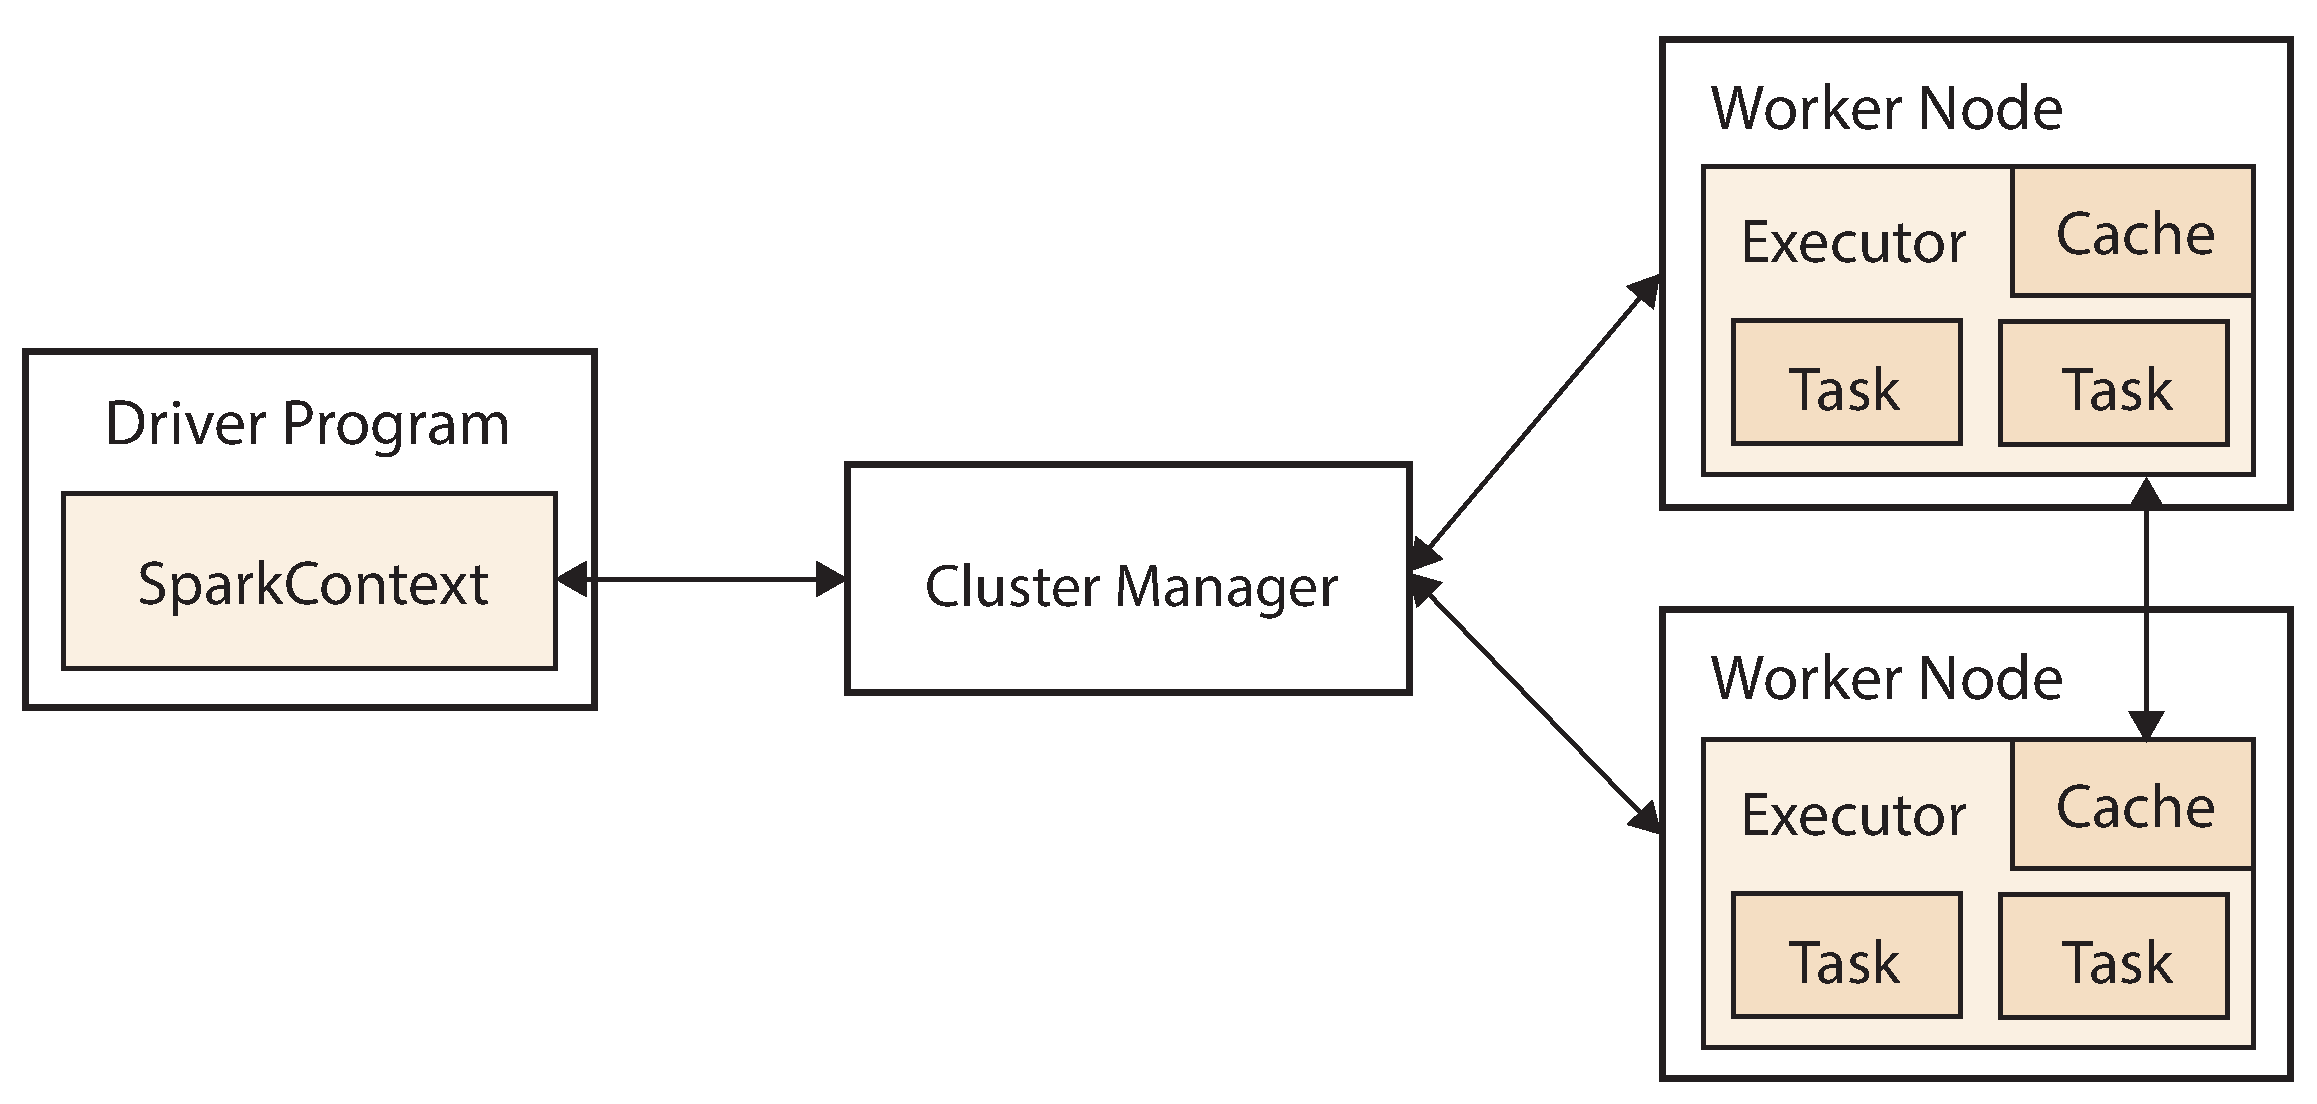
\includegraphics[scale=0.32]{imagens/spark_arquitetura.pdf}
    \end{center}
    \small{Fonte: Adaptado de (\citeauthor{frampton2015mastering}, 2015, p. 8)}
    \label{fig:spark_arquitetura}
\end{figure}


O \textit{Cluster Manager} é encarregado de gerenciar as máquinas que serão utilizadas como \textit{Workers} durante o processamento das aplicações Spark. De acordo \cite{chambers2018spark}, são esses gerenciadores de \textit{Clusters} que concedem recursos para completar a execução da aplicação. Por padrão, o Spark inclui um gerenciador de recursos \textit{stand-alone} incluso na distribuição  do \textit{framework}. Além deste, há suporte para o Apache Hadoop YARN\footnote{Disponível em: https://hadoop.apache.org}, Apache Mesos\footnote{Disponível em: http://mesos.apache.org/} e Kubernetes\footnote{Disponível em: https://kubernetes.io/}.

Os \textit{Workers} são os nodos que realizam o processamento das \textit{tasks} necessárias para a computação do \textit{job}, sendo estes nodos os encarregados de armazenar os \textit{Executors} do Spark. Um \textit{Executor} consiste em um processo JVM isolado lançado pelo Spark, com o objetivo executar o código delegado pelo \textit{Driver Program} e reportar seu \textit{status}. Além disso, cada \textit{Executor} possui sua região de memória isolada capaz de prover o armazenamento em memória para RDDs. O gerenciamento deste espaço é feito de forma autônoma pelo próprio \textit{Executor}, utilizando o algoritmo LRU.

\subsection{Modelo de Divisão da Memória}
O espaço de memória alocado e gerenciado por cada \textit{Executor} pode ser dividio em  três principais regiões de memória: Reservada, Usuário e Spark. Esta divisão pode ser observada na Figura \ref{fig:spark_memoria_arquitetura}.

\begin{figure}[!ht]
    \caption{Arquitetura da Memória do Apache Spark.}
    \begin{center}
        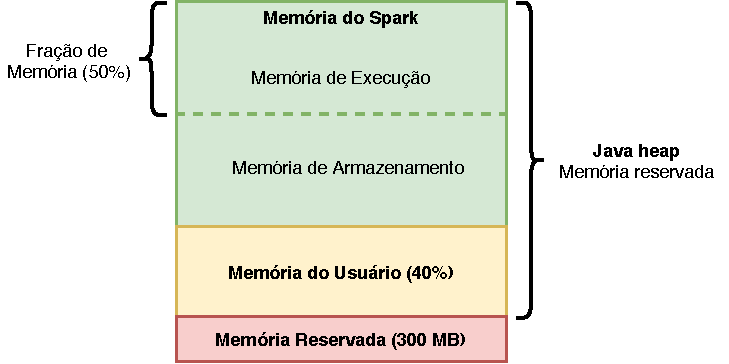
\includegraphics{imagens/modelo_memoria_spark_corrigido_2.pdf}
    \end{center}
    \small{Fonte: Adaptado de \cite{UnifiedMemoryManager}}
    \label{fig:spark_memoria_arquitetura}
\end{figure}

A Memória Reservada é uma região alocada estaticamente, via código fonte, com tamanho igual a 300MB, não sendo incluída no cálculo de memória disponível no Spark. O principal objetivo dessa área de memória é armazenar objetos internos do Spark.

A Memória do Usuário é a fração do \textit{Java heap} disponível para o usuário utilizar. Nessa região são armazenadas as estruturas, objetos e dados criados durante o desenvolvimento de aplicações Spark. O tamanho desta região corresponde a 40\% da memória disponível após a alocação da memória reservada. É importante ressaltar que o gerenciamento desta memória não é realizado pelo Spark, sendo delegado inteiramente ao \textit{Garbage Collector} (GC) da JVM.

A Memória do Spark é a região efetivamente controlada e gerenciada pelo Spark e GC da JVM. O tamanho desta região corresponde à fração de 60\% da memória disponível do \textit{Java heap} após a alocação da Memória Reservada. Esta região é subdividida em duas porções: Memória de Execução e Memória de Armazenamento, cada qual com 50\% do tamanho da área inicial da Memória do Spark. 

A Memória de Execução é responsável por armazenar os objetos e dados resultantes de operações intermediárias durante a execução de \textit{tasks}. Já a Memória de Armazenamento abriga os dados computados e assinalados para serem mantidos em memória, espaço para a deserialização de dados e armazenamento das variáveis de \textit{broadcast}. Estas variáveis têm como objetivo compartilhar o estado da execução do \textit{job} entre os nodos do \textit{cluster}.

A forma em que a divisão do \textit{Java heap} é feita variada de acordo com a versão do Spark. Assim, em versões 1.5.x e anteriores do Spark, a divisão de memória era realizada de forma estática, isto é, alocava-se 50\% do espaço de memória para cada subdivisão, independentemente da necessidade. A partir da versão 1.6 foi implementado o balanceamento dinâmico da divisão de memória, permitindo que a quantidade de memória disponível em cada subespaço seja alocada de acordo com as necessidades no momento da execução. 

Se durante a execução de uma determinada tarefa não houver memória suficiente disponível na Memória de Execução, o Spark pode alocar a memória extra necessária no espaço livre da Memória de Armazenamento. Caso a Memória de Armazenamento esteja esgotada, blocos desta região podem ser removidos a fim de disponibilizar espaço para a conclusão da tarefa em questão. 

Em casos onde há necessidade de armazenar novos dados na Memória Armazenamento e o espaço desta região estiver esgotado, o Spark pode remanejar uma porção livre da Memória de Execução para o armazenamento. Caso não seja possível realizar esta operação, o Spark poderá remover blocos da Memória de Armazenamento a fim de disponibilizar espaço. A remoção desses blocos de memória é realizada seguindo a ordem definida pelo algoritmo LRU.

Embora a divisão da memória alocada para o Spark seja determinada em tempo de execução, o espaço de memória total ocupado pela \textit{Java heap} pode ser ajustado. Cada aplicação Spark em execução pode ter uma configuração de memória associada, independente das demais. Estas configurações são metadados da aplicação bem como características de execução \cite{chambers2018spark}, contendo informações que serão utilizadas pelo Spark para configuração do ambiente de execução.

Por padrão, o Spark busca um arquivo denominado \textit{spark-defaults.conf}, responsável por armazenar as configurações no formato chave-valor. Através deste arquivo, configurações como tamanho da memória utilizada pela \textit{Java heap} e percentual de divisão do espaço entre a Memória de Armazenamento e a Memória de Execução, dentre outras, podem ser ajustadas pelo usuário.

Durante a execução de aplicações, é possível monitorar a quantidade de memória utilizada, assim como o \textit{status} da execução da aplicação, através de uma API REST (\textit{Representational State Transfer}). Por meio deste serviço, os usuários podem monitorar aplicações em execução, além de permitir a realização de construções de visualizadores customizados \cite{souravgulati2017}.

\subsection{Gerenciamento da Memória Disponível}
O Spark é um \textit{framework} para processamento de grandes volumes de dados em memória principal. Consequentemente, exige um bom gerenciamento da memória disponível, a fim de otimizar sua ocupação e alcançar melhor desempenho. De forma geral, o gerenciamento da memória realizado pelo Spark é composto por três classes principais: \textit{MemoryManager}, \textit{BlockManager} e \textit{MemoryStore}. O diagrama de inicialização destas classes é exibido na Figura \ref{fig:criacao-memorystore}.

A classe \textit{SparkEnv} é responsável por armazenar as configurações globais do \textit{cluster} e compartilhar essas informações com todos os nodos Spark. A partir desta classe, cria-se as classes \textit{MemoryManager}, \textit{SerializerManager} e \textit{BlockManager}.

A classe \textit{MemoryManager} visa oferecer uma abstração da memória, de modo a compartilhar o espaço disponível entre as porções de Memória de Armazenamento e Memória de Execução. Assim, existe uma instância dessa classe em execução em cada \textit{Executor} ativo no \textit{cluster} Spark.

\begin{figure}[!ht]
    \caption{Fluxo de Inicialização do Gerenciamento de Memória do Spark}
    \begin{center}
        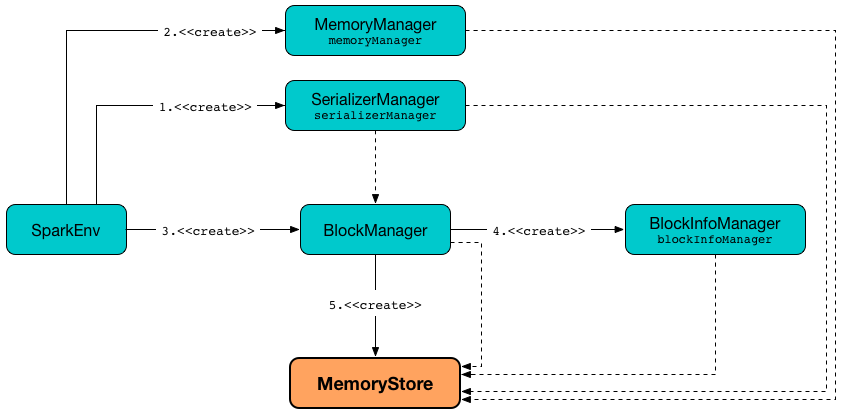
\includegraphics[scale=0.52]{imagens/criacao-memorystore.png}
    \end{center}
    \small{Fonte: \cite{laskowski2017mastering}}
    \label{fig:criacao-memorystore}
\end{figure}

A classe \textit{SerializerManager} é responsável por configurar o serializador utilizado pelo Spark, incluindo aquele utilizado nas operações de \textit{shuffle}. Esta classe é utilizada para a criação do \textit{BlockManager} e do \textit{MemoryStore}.

A classe \textit{BlockManager} oferece interfaces para realizar a adição e recuperação de blocos de dados localmente no \textit{Executor} e remotamente, isto é, em outros nodos do \textit{cluster} \cite{BlockManagerSpark}. A adição e recuperação desses blocos pode ser realizada em diferentes fontes de armazenamento, tais como memória principal e armazenamento estável.

O \textit{BlockManager} é responsável também, pela criação do \textit{BlockInfoManager} a qual tem como objeto rastrear os metadados dos blocos de dados de maneira individual, os quais são utilizados para informar a localização do bloco, isto é, memória ou disco. Ainda, é função do \textit{BlockInfoManager} fornercer os \textit{locks} de leitura e escrita desses blocos.

Na classe \textit{MemoryStore} encontram-se os métodos e variáveis para armazenamento e remoção de informações da memória \cite{MemoryStoreSpark}. Estas informações podem ser \textit{Arrays} de objetos Java desserializados ou \textit{Buffers} de \textit{bytes} serializados. Além disso, cabe a esta classe implementar a política de gerenciamento de memória utilizada pelo Spark: o algoritmo LRU.

O LRU é um algoritmo clássico para gerenciamento de memória em diversos sistemas. No Spark, a implementação deste algoritmo é realizada utilizando uma lista encadeada (\textit{LinkedHashMap}) provida nativamente pela distribuição Java. Através desta estrutura, o Spark mantém uma estrutura de lista encadeada contendo os dados de maneira ordenada por acesso. Cada vez que uma determinada posição dessa lista é acessada, esta posição é movida para o final da lista. Por consequência, as posições mais recentemente acessadas são encontradas ao final desta lista encadeada.

A estrutura de lista é iniciada com 32 posições e um fator de carregamento de 75\%. Isso significa que, ao atingir 75\% da capacidade de ocupação, novas posições começam a ser alocadas dinamicamente pela JVM. Uma particularidade dessa lista está relacionada à forma como a mesma deve ser manipulada em ambientes \textit{multithread}. Nesses ambientes, o acesso deve ser feito de maneira sincronizada entre as \textit{threads} em execução, pois a implementação não é realizada de maneira \textit{thread-safe}. Essa sincronização busca manter a ordenação, uma vez que há alteração nas posições armazenadas na lista quando ocorre acesso a mesma.

A sincronização entre as \textit{threads} em execução no Spark é realizada através de um \textit{lock} global do objeto. Deste modo, apenas uma \textit{thread} consegue realizar a escrita, leitura ou remoção de um bloco de dado a partir da estrutura, evitando condições de corrida (\textit{race condition}) entre as \textit{threads}. Entretanto, esta sincronização pode acarretar em uma sobrecarga para a aplicação, uma vez que durante essas operações apenas uma \textit{thread} consegue manipular a estrutura, bloqueando as demais.

Cada Spark \textit{Worker} executando no \textit{cluster} possui suas próprias estruturas para controlar as regiões de memória. Assim, cada nodo Spark gerencia sua memória de forma autônoma e sem dependências externas. Além disso, devido à distribuição dos dados do RDDs entre os nodos, o momento em que blocos de memória deverão ser removidos pode variar entre diferentes nodos. 

\section{Apache ZooKeeper} \label{sec:Zookeeper}
O Apache ZooKeeper é um \textit{framework} de código aberto cujo objetivo é prover soluções para problemas de coordenação em grandes conjuntos de nodos \cite{hunt2010Zookeeper}. Através deste, é possível coordenar grupos de nodos entre si e manter o compartilhamento de informações com técnicas de sincronização robustas.

O ZooKeeper realiza o processo de coordenação através de um \textit{namespace} hierárquico compartilhado organizado de maneira semelhante a um sistema de arquivos padrão. Entretanto, diferente dos sistemas de arquivos, os nodos responsáveis por armazenar os dados, denominados de \textit{znodes}, são estruturas similares a arquivos e diretórios projetados para serem armazenados em memória principal. Um \textit{namespace} do \textit{znode} pode conter dados associados e referências a outros \textit{znodes}.  A Figura \ref{fig:ZookeeperNamespace} exibe um nodo denominado de \textit{"/"}, o qual possui dois outros nodos associados, exemplificando a arquitetura utilizada no \textit{namespace}.

\begin{figure}[!ht]
    \caption{Estrutura de \textit{namespace} do Apache ZooKeeper}
    \begin{center}
        \includegraphics[scale=0.5]{imagens/Zookeeper-namespace.png}
    \end{center}
    \small{Fonte: \cite{haloi2015apache}}
    \label{fig:ZookeeperNamespace}
\end{figure}

Um \textit{znode} mantém uma estrutura do estado atual dos dados armazenados, a qual inclui o número da versão, o \textit{Action Control List} (ACL) e um \textit{Timestamp}. O número da versão representa a quantidade de vezes que os dados armazenados pelo \textit{znode} foram alterados.  O ACL é o mecanismo de autenticação, assegurando quais nodos do \textit{cluster} podem realizar operações de escrita e leitura. O \textit{Timestamp} descreve o tempo decorrido desde a criação do nodo até o momento da modificação dos dados armazenados. 

Uma importante característica do ZooKeeper é a capacidade de oferecer suporte a \textit{Watchers}, permitindo que clientes possam receber notificações ocorridas em um determinado \textit{znode}. A manutenção da comunicação entre o \textit{Master} e os clientes é realizada através de mensagens \textit{heartbeat}, as quais garantem que a conexão com os clientes entra-se ativa.

Uma mudança em um \textit{znode} consiste em uma modificação nos dados associados a este nodo ou uma alteração em um de seus nodos filhos \cite{junqueira2013Zookeeper}. Através dos \textit{znodes}, as aplicações podem oferecer suporte a serviços de sincronização, fila de mensagens, além de gerenciamento de configuração do \textit{cluster}.

Juntamente com seu sistema de \textit{znodes}, o ZooKeeper oferece uma API com suporte oficial para as linguagens Java e C, a fim de realizar a criação de aplicações cliente. Através destes clientes, pode-se conectar, manipular dados associados aos \textit{znodes}, coordenar operações e interagir com ZooKeeper.


\section{Trabalhos Relacionados} \label{sec:trab-relacionados}
O algoritmo utilizada para o gerenciamento do espaço disponível pode afetar diretamente o desempenho do \textit{framework} durante o processamento de aplicações. Nesse sentido, alternativas têm sido pesquisadas e desenvolvidas buscando aumentar a eficiência do Apache Spark.

O trabalho desenvolvido por \cite{wang2015new} apresenta uma abordagem para analisar o comportamento do Spark ao realizar acessos à memória visando melhorar a ordem da execução de ações nos RDDs. Para tanto, os autores utilizam um algoritmo guloso para encontrar a melhor sequência para executar as ações aplicadas aos RDD, uma vez que o processamento de uma ação independe das demais. Juntamente com este algoritmo, a abordagem tem como objetivo calcular um peso do RDD em uma \textit{task}. O cálculo deste peso considera 6 critérios: tamanho dos dados de entrada do RDD, custo de computação, frequência de reutilização, tamanho do conjunto de dados de saída da transformação aplicada, ciclo de vida do RDD (isto é, por quanto tempo este é manipulado) e custo de armazenar o RDD em disco. Em seguida, é apresentado um novo algoritmo denominado de ASRD (\textit{Action's Sequence and RDD Weight}), o qual combina a análise da execução aliada ao peso do RDD calculado. Os autores não especificam a versão do Spark utilizada, tampouco o ambiente usado para validação do método proposto. Entretanto, os autores do trabalho não apresentaram resultados em termos percentuais, limitando-se a afirmar que a metodologia proposta obteve um ganho na taxa de acerto de acesso à memória, quando comparado ao LRU.

Em \cite{duan2016selection} é  apresentado um algoritmo para a seleção de RDDs a serem armazenados em \textit{cache} baseado na frequência de utilização dos RDDs na aplicação. Dessa forma, remove-se a necessidade do desenvolvedor de decidir qual RDD deve ser mantido em \textit{cache} para ser reutilizado posteriormente. Quando a memória alcança o seu limite disponível, blocos são removidos de acordo com uma nova política proposta pelos autores: o algoritmo \textit{Weight Replacement}. Esse algoritmo consiste na atribuição de um peso, calculado a partir do custo de recomputação da partição, além da frequência de utilização e tamanho da partição. A proposta apresentada foi implementada no Spark 1.1.0 e validada utilizando 17 \textit{datasets} reais. De acordo com os autores, o algoritmo proposto obteve melhores resultados quando comparado ao LRU, reduzindo o tempo de execuçāo da aplicação \textit{PageRank}. Entretanto, não são apresentados percentuais deste ganho de desempenho. 

Em \cite{zhang2017intelligent}, os autores apresentam uma estratégia inteligente para \textit{checkpointing} e remoção de blocos da memória pelo Spark. Tal estratégia consiste na atribuição de uma prioridade \textit{P} para cada RDD, calculada a partir do tempo de recomputação, do tempo de \textit{checkpointing} e do grau de dependência entre os RDDs. Assim, quanto maior o valor de \textit{P}, maior deve ser a prioridade do RDD permanecer em memória. A validação desta proposta foi realizada utilizando o Spark 1.5 em 4 servidores, com a memória variando entre 5G, 10G e 20G. De acordo com os autores do trabalho, o resultado obtido demonstra um ganho médio de desempenho de 13,63\% quando comparado ao LRU.

O trabalho realizado por \cite{xu2016neutrino} apresenta um gerenciador de \textit{cache} distribuído denominado de \textit{Neutrino}. Esse gerenciador é responsável por tomar decisões relativas ao armazenamento dos RDDs com base em configurações do \textit{cluster} e na execução da aplicação. Para tanto, o \textit{Neutrino} analisa a ordem em que os RDDs serão utilizados e calcula o menor tempo de execução possível do \textit{Job}. Esse gerenciador foi implementado como uma extensão do Spark 1.5.0. De acordo com os autores, a solução proposta apresenta resultados promissores quanto a sua utilização. 

Em \cite{geng2017lcs} é demonstrada uma estratégia denominada \textit{Least Cost Strategy} (LCS) para a remoção de blocos de memória, a qual integra o custo de recuperação da partição em cache e a lógica de execução da aplicação. Este algoritmo combina o tempo necessário para criar, remover e recomputar cada partição dos RDDs juntamente com uma frequência de reutilização de cada partição. A implementação dessa estratégia foi realizada utilizando o Spark 1.5.2. Conforme os autores, o LCS consegue um desempenho em torno de 30\% melhor que o LRU.

Em \cite{yang2018intermediate}, os autores apresentam um algoritmo para determinar e armazenar adaptativamente os \textit{datasets} intermediários mais valiosos, isto é, aqueles que poderão ser reutilizados no futuro. Assim, este algoritmo automatiza a decisão de quais RDDs devem ser persistidos em memória, analisando o DAG gerado pelo Spark durante a execução do \textit{job}. O algoritmo foi implementado utilizando o Spark 2.2.1 e sua validação ocorreu utilizando a aplicação \textit{Ridge Regression}. Segundo os autores, o algoritmo proposto consegue reduzir em 12\% o trabalho necessário para realizar as recomputações dos RDDs removidos.

No trabalho desenvolvido por \cite{inagaki2018adaptive}, é apresentada uma metodologia de \textit{cache} adaptativa para o Spark, a qual modifica o comportamento dos métodos de armazenamento e remoção de dados da \textit{cache}, dependendo das características da aplicação. Em situações onde os dados da aplicação são frequentemente movidos da memória para o disco, esta abordagem de \textit{cache} adaptativo move estes dados diretamente para o armazenamento estável. Além disso, se estes dados armazenados no disco são requeridos pela aplicação, o mecanismo de \textit{cache} adaptativo carrega os dados necessários diretamente para a Memória de Execução do Spark. Estas ações de carga de \textit{cache} são realizadas analisando a execução da aplicação ao invés das dependências entre os RDDs. A implementação desta estratégia foi realizada utilizando a versão 2.0.1 do Spark. De acordo com os autores, este mecanismo de gerenciamento de \textit{cache} reduziu em 33\% o tempo de execução do \textit{benchmark} K-Means, quando comparado ao LRU utilizando o nível de armazenamento Memória e Disco nativo do Spark. 

É possível encontrar na literatura algoritmos e soluções que têm como objetivo melhorar a forma na qual o Spark realiza o processamento de aplicações onde há a reutilização de dados em computações futuras, uma vez que o algoritmo LRU pode acarretar em degradação no desempenho do \textit{framework} nesta classe de aplicações. Entretanto, quando analisamos tais soluções, duas características ficam evidentes: versão do Spark e metodologia utilizada. 

A primeira característica está relacionada à versão utilizada para implementação e validação, onde geralmente os trabalhos concentram-se em versões defasadas e com um modelo de memória diferente daquela utilizada por versões mais novas do Spark. A segunda característica encontrada em trabalhos disponíveis na literatura relaciona-se com as soluções propostas, onde comumente foca-se em algoritmos estáticos e reativos. Embora as soluções encontradas utilizem métricas colhidas a partir da aplicação, estas soluções tendem a executar apenas quando há necessidade de liberação de memória.

Diferentemente dos algoritmos e soluções encontradas na literatura, este trabalho tem como objetivo implementar um modelo para realizar o Gerenciamento Dinâmico da Memória utilizada pelo Spark, em versões 2.x do \textit{framework}. Esta solução tem como foco as aplicações onde há reutilização de dados em computações futuras. Para tanto, o modelo proposto é composto por dois componentes: um algoritmo de gerenciamento de memória e um agente de monitoramento.

O algoritmo de gerenciamento de memória visa extrair a frequência de reutilização dos RDDs da aplicação e combiná-la com o algoritmo LRU. Já o agente de monitoramento tem como objetivo obter o \textit{status} e informações da aplicação em execução e decidir se deve ocorrer a remoção dos dados em \textit{cache}. Através deste modelo, busca-se corrigir as deficiências encontradas no algoritmo LRU no processamento de aplicações onde há reutilização de dados.
\chapter{Gerenciamento Dinâmico da Memória} \label{cap:implementacoes}
A concepção do Gerenciamento Dinâmico da Memória em Aplicações com Reuso de Dados no Apache Spark proposto por este trabalho foi realizada de forma modular. Deste modo, duas implementações foram previamente desenvolvidas até culminar na versão final do algoritmo utilizado para gerir as partições de RDDs em memória na implementação do Gerenciamento Dinâmico. A Figura \ref{fig:fluxo-evolucao-trabalho} ilustra, de forma resumida, a evolução do trabalho, descrevendo o funcionamento de cada algoritmo e as razões para sua alteração.

\begin{figure}[!ht]
    \caption{Fluxo Evolutivo do Algoritmo de Gerenciamento Dinâmico da Memória.}
    \begin{center}
        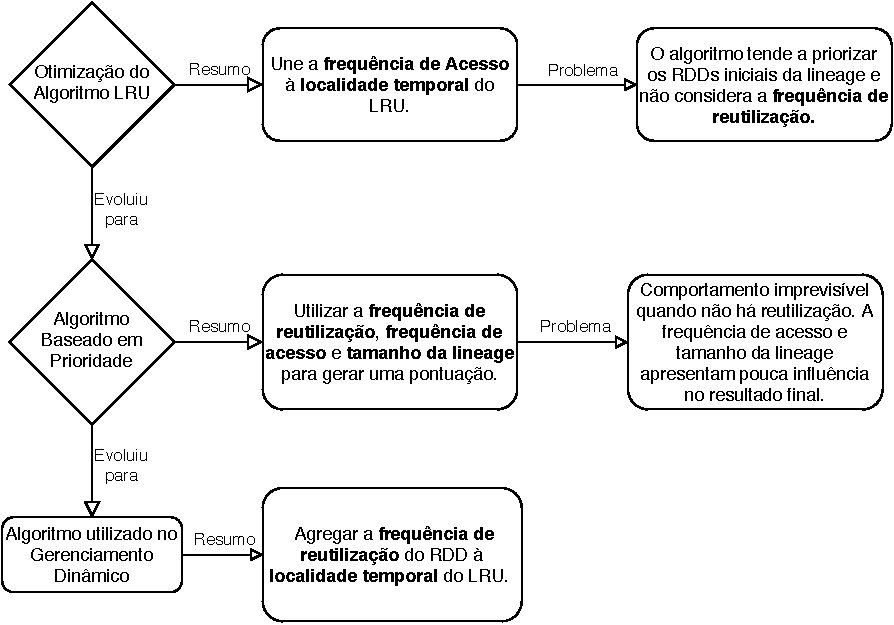
\includegraphics[scale=1]{imagens/fluxo-evolucao-trabalho.pdf}
    \end{center}
    \small{Fonte: Próprio autor.}
    \label{fig:fluxo-evolucao-trabalho}
\end{figure}

O primeiro algoritmo desenvolvido, a Otimização do Algoritmo LRU, tinha como objetivo agregar a Frequência de Acesso do RDD juntamente com a ordenação temporal provida pelo LRU. A Seção \ref{sec:lru-mfu} dedica-se a descrever o funcionamento deste algoritmo, junto com sua respectiva implementação. Ainda nesta Seção, são detalhados os experimentos realizados e os resultados obtidos.

A partir dos problemas identificados na Otimização do Algoritmo LRU, um segundo algoritmo foi desenvolvido, sendo denominado de Algoritmo Baseado em Prioridades. Este algoritmo visava unir a Frequência de Acesso, o Tamanho da \textit{Lineage} e a Frequência de Reutilização dos RDDs a fim de gerar uma pontuação, simbolizando a prioridade deste RDD estar em memória. Detalhes relativos ao seu funcionamento, implementação, experimentos e resultados são explanados na Seção \ref{sec:alg-pesos}

Utilizando como base os dois algoritmos previamente desenvolvidos, uma nova otimização do algoritmo LRU foi desenvolvida com o objetivo de corrigir as deficiências do LRU e dos algoritmos anteriores. Esta otimização tem como finalidade agregar a localidade temporal do LRU à Frequência de Reutilização dos RDDs manipulados no \textit{job}, sendo este algoritmo utilizado no \textbf{Gerenciamento Dinâmico da Memória}. A Seção \ref{sec:gerenc-dinamico} é destinada a expor este algoritmo, juntamente com os dois componentes utilizados para implantar o Gerenciamento Dinâmico da Memória, descrevendo as nuances relativas ao funcionamento e implementação no Spark. A Seção é finalizada descrevendo os experimentos e resultados obtidos pelo Gerenciamento Dinâmico.   



\section{Otimização do Algoritmo LRU} \label{sec:lru-mfu}
O algoritmo LRU utilizado nativamente pelo Spark pode ocasionar uma possível degradação no desempenho da ferramenta no processamento de aplicações com reutilização de dados. Visando sanar esta deficiência, uma primeira modificação na política de gerenciamento de memória foi implementada, a qual consistia em uma otimização do algoritmo LRU utilizado pelo \textit{framework}.

A otimização desenvolvida consiste em um algoritmo que combina a \textbf{localidade temporal} do LRU com a \textbf{frequência de acesso} dos RDDs utilizados na computação do \textit{job}. A frequência de acesso tem como objetivo descrever a quantidade de vezes a qual cada RDD é utilizado no processamento da aplicação. 

Para tanto, este algoritmo analisa o \textit{job} gerado pelo \textit{DAGScheduler} a fim de identificar os RDDs manipulados e obter suas respectivas frequências de acesso. A partir destas informações, mantém-se uma lista de partições dos RDDs ordenadas pela frequência de acesso. Uma vez realizada esta ordenação, conforme as novas partições dos RDDs são carregadas para a memória principal, estas partições são armazenadas de maneira ordenada pela frequência de acesso, de maneira a manter a ordenação inicial.

Em cenários onde há duas ou mais entradas com a mesma frequência, estas são sub-ordenadas de acordo com o algoritmo LRU. Assim, garante-se que os RDDs mais frequentemente utilizados no processamento serão os últimos a serem removidos da memória e, em caso de empate, é removida a partição onde o acesso ocorreu há mais tempo.

A implementação deste algoritmo implica na obtenção da frequência de acesso de cada RDD da aplicação e na difusão desta informação entre todos os \textit{Executors} da aplicação. As frequências de acesso dos RDDs são obtidas através do escalonador do Spark, o \textit{DAGScheduler}, antes de iniciar a execução da aplicação. Para isso, navega-se recursivamente entre o plano de execução para a computação do \textit{job} gerado pelo escalonador, com o objetivo de identificar os RDDs utilizados. O resultado desta etapa consiste em uma lista contendo todos os RDDs manipulados no \textit{job}. Em seguida, a lista gerada é utilizada para obter a frequência de acesso de cada RDD, analisando a \textit{lineage} de cada RDD. 

Ao final do processo de análise da \textit{lineage}, uma estrutura de  \textit{HashMap} é gerada, mapeando cada RDD do \textit{job} com sua respectiva frequência de acesso. Assm, o consumo extra de memória será a quantidade máxima de entradas nesta estrutura de \textit{HashMap}, igual ao número de RDDs manipulados na aplicação. Cada entrada desse \textit{HashMap} possui dois inteiros, onde o primeiro inteiro corresponde ao identificador do RDD e o segundo a frequência de acesso deste mesmo RDD.

Após a obtenção das frequências de acesso, o próximo passo consiste em difundir esta lista contendo as frequências de acesso entre os \textit{Executors} do \textit{cluster}. A etapa de difusão se faz necessária uma vez que apenas através do \textit{Driver} da aplicação, o qual hospeda o \textit{DAGScheduler}, é possível obter informações referentes à frequência de acesso a cada RDD do \textit{Job}. 

A difusão é realizada de maneira síncrona entre todos os \textit{Executors}. O sincronismo na comunicação entre o \textit{Driver} e os \textit{Executors} garante que os dados referentes aos RDDs estejam em todos os nodos antes de seu efetivo uso. Em contrapartida, a utilização deste tipo de comunicação acarreta em um atraso no início da execução. Isto ocorre devido ao comportamento das chamadas síncronas, as quais são bloqueantes, isto é, nenhum outro processamento é realizado até a conclusão da comunicação. Consequentemente, há uma sobrecarga na execução da aplicação, atrasando o início do processamento \textit{job} em até 2 segundos, por comunicação realizada.

Esta otimização do algoritmo LRU teve como objetivo priorizar aqueles RDDs com maior frequência de acesso dentro do \textit{job}, postergando sua remoção tanto quanto possível. Entretanto, conforme a \textit{lineage} cresce, os RDDs iniciais tendem a apresentar uma alta frequência de acesso, uma vez que estes RDDs são computados diversas vezes para originar novos RDDs. 

Além disso, este algoritmo não considera um importante parâmetro para decidir quais partições remover: a frequência de reutilização do RDD. Este parâmetro tem relevância, uma vez que a remoção de um RDD com uma alta frequência de reutilização implica em sua completa recomputação a cada novo acesso, podendo implicar em uma degradação no desempenho do \textit{framework}. 

Ademais, quando analisadas as soluções encontradas na literatura, a frequência de reutilização de um RDD se mostra uma importante métrica para o planejamento de algoritmos focados em aplicação com reutilização de dados. Junto com a frequência de reutilização, métricas auxiliares podem ser agregadas, tais como custo computacional, a fim de tornar o gerenciamento da memória mais eficiente.

\subsection{Experimentos e Resultados}
A fim de validar o algoritmo desenvolvido, foram conduzidos experimentos em um ambiente distribuído visando avaliar seu impacto no tempo de execução das aplicações. Os experimentos foram realizados utilizando os algoritmos  \textit{PageRank} e \textit{K-Means} como \textit{benchmarks}. Estes \textit{benchmarks} foram selecionados, uma vez que cada um deles apresenta um comportamento diferente no acesso à memória. 

Uma característica comum aos dois \textit{benchmarks} é a reutilização de dados em computações futuras. O \textit{PageRank} visa classificar \textit{links} de acordo com suas ligações, a fim de gerar uma relevância para um determinado \textit{link}. O \textit{K-Means} consiste em agrupar os dados de entrada em $K$ grupos baseados em suas características, sendo este um algoritmo de \textit{machine learning} não supervisionado. Em todos os experimentos, os \textit{benchmarks} foram implementados pela suíte Intel HiBench \cite{huang2010hibench}.

O ambiente utilizado foi a plataforma Grid'5000 \cite{bolze2006grid}, executando os \textit{benchmarks} em um \textit{cluster} com 5 nodos configurados da seguinte maneira: 1 Spark \textit{Master}; 2 Spark \textit{Workers}; 1 \textit{HDFS Namenode} e 1 \textit{HDFS Datanode}. Cada nodo do sistema era composto por um Intel Xeon X3440 @2.53GHz (4 \textit{cores}/CPU) e 16GB de memória RAM, conectados via \textit{ethernet} 1 Gbps. O sistema operacional utilizado foi o Debian 8, juntamente com Java JDK 1.8.187, Spark 2.2.0 e Hadoop 2.7.1. Além disso, cada Spark \textit{Executor} utilizou duas configurações de memória: 1GB, sendo 366,6 MB para a Memória e armazenamento e 2 GB, dos quais 912,3MB eram dedicados ao armazenamento de dados. Estas configurações de memória tinham como objetivo estressar o gerenciamento do espaço disponível, a fim de verificar o impacto do algoritmo no tempo de execução das aplicações quando comparado ao LRU nativo do Spark. Por fim, os resultados obtidos são a média aritmética de 20 execuções.

Os resultados obtidos por este algoritmo são apresentados na Tabela \ref{tab:alg-erad}. Estes resultados demonstraram um desempenho similar ao LRU, apresentando pouca variação no tempo de execução. Embora os tempos obtidos sejam semelhantes, a modificação do LRU é penalizada pela necessidade de comunicação entre os nodos do \textit{cluster} para seu funcionamento. Analisando os \textit{logs} gerados pela aplicação, cada comunicação síncrona pode levar até 2 segundos para ser executada, sendo este tempo diluído no tempo total de execução da aplicação.

\begin{table}[!ht]
    \centering
    \caption{Otimização do LRU: Tempos de Execução dos \textit{Benchmarks}}
        \begin{tabular}{ccccc}
            \hline
            Benchmark & Algoritmo & \begin{tabular}[c]{@{}c@{}}Memória \\ Disponível\end{tabular} & \begin{tabular}[c]{@{}c@{}}Tempo de \\ Execução (em s)\end{tabular} & \begin{tabular}[c]{@{}c@{}}Desvio \\ Padrão (em s)\end{tabular} \\ \hline
            \multirow{4}{*}{K-Means} & \multirow{2}{*}{LRU} & 1 GB & 47,78 & 0,88 \\
             &  & 2 GB & 25,48 & 0,30 \\ \cline{2-5} 
             & \multirow{2}{*}{Otimização do LRU} & 1 GB & 46,26 & 2,68 \\
             &  & 2 GB & 25,21 & 0,41 \\ \hline
            \multirow{4}{*}{PageRank} & \multirow{2}{*}{LRU} & 1 GB & 179,21 & 2,48 \\
             &  & 2 GB & 153,91 & 2,50 \\ \cline{2-5} 
             & \multirow{2}{*}{Otimização do LRU} & 1 GB & 176,93 & 3,43 \\
             &  & 2 GB & 152,78 & 1,85 \\ \hline
        \end{tabular}
    \label{tab:alg-erad}
\end{table}

A necessidade de efetuar comunicação síncrona entre o \textit{Driver} da aplicação e os \textit{Executors}, para cada \textit{job} da aplicação, faz com que o processamento não seja iniciado até que a transmissão das informações para todos os nodos seja concluída. Esta comunicação é realizada independente da necessidade e, portanto, acarreta em um aumento do tempo de execução.

\section{Algoritmo Baseado em Prioridades} \label{sec:alg-pesos}
Com o objetivo de resolver as deficiências identificadas na primeira otimização do algoritmo LRU (Seção \ref{sec:lru-mfu}), um novo algoritmo foi desenvolvido. Este algoritmo visa agregar três diferentes métricas, a saber: a Frequência de Reutilização, a Frequência de Acesso e o Tamanho da \textit{Lineage} dos RDDs. O algoritmo busca determinar uma prioridade para cada RDD ser mantido em memória, sendo esta prioridade simbolizada por uma pontuação.


\subsection{Descrição do Algoritmo}
O algoritmo tem como objetivo obter métricas as quais serão utilizadas para gerir a memória do Spark. Assim, após a computação do plano de execução pelo \textit{DAGScheduler}, o estágio resultante é utilizado para extrair métricas da aplicação e calcular a pontuação de cada RDD do \textit{job}. 

A partir do estágio gerado, navega-se recursivamente entre as dependências do \textit{job}, a fim de identificar os RDDs manipulados. Na sequência, é realizada a extração das métricas Frequência de Reutilização, Frequência de Acesso e Tamanho da \textit{Lineage}, a partir dos RDDs mapeados previamente.

Uma vez realizada a extração das métricas relativas aos RDDs do \textit{job}, o próximo passo consiste em analisar os resultados. Nessa análise, são calculadas as pontuações dos RDDs utilizados na computação do \textit{job}, simbolizando a prioridade deste RDD ser mantido em memória. A pontuação obtida é calculada a partir da frequência de reutilização multiplicada pela média aritmética da frequência de acesso somada ao tamanho da \textit{lineage}, conforme exibe a Equação \ref{eq:priorityCalculation}.

A Equação \ref{eq:priorityCalculation} foi concebida com a intenção de priorizar os RDDs com maior número de reutilizações dentro do \textit{job}, em detrimento aos demais. Em situações onde não há reutilização do RDD, o algoritmo calcula uma pontuação para cada RDD baseando-se na média aritmética entre a frequência de acesso e o tamanho da \textit{lineage}. O estudo da correlação da equação proposta é discutida na Seção \ref{subsec:analise-convergencia}.

\begin{equation}
    \label{eq:priorityCalculation}
    P = n\_reusos * (0,5 * freq\_acesso + 0,5 * tam\_lineage)
\end{equation}

Após concluídos o processamento e o cálculo das prioridades dos RDDs, o resultado final consiste em uma lista mapeando todos os RDDs com suas respetivas pontuações. Esta lista é armazenada no \textit{Driver}. A difusão da lista com as pontuações de cada RDD é realizada entre os nodos do \textit{cluster} sob demanda. Isso significa que a comunicação entre o \textit{Executor} e o \textit{Driver} irá ocorrer apenas quando a memória desse \textit{Executor} estiver sobrecarregada e necessitando realizar a remoção de partições da memória. 

Em caso de sobrecarga, o \textit{Executor} irá solicitar a lista contendo a pontuação de cada RDD do \textit{job}. Essa requisição ocorre em duas situações: quando a lista com as pontuações está vazia e quando o identificador de uma partição não é encontrado. O \textit{status} de lista vazia significa que o processamento da aplicação começou recentemente e nenhum bloco foi removido. A ausência de um identificador na lista indica que um novo \textit{job} iniciou e novos RDDs foram manipulados, necessitando que a lista de pontuações seja atualizada no \textit{Executor}.  

\subsection{Métricas utilizadas}
O Algoritmo Baseado em Prioridade foi concebido com o objetivo de agregar três métricas e, a partir destas, determinar a ordem em que as partições de RDDs serão removidas. Assim, utiliza-se a Frequência de Acesso, o Tamanho da \textit{Lineage} e a Frequência de Reutilização de cada RDD que será manipulado no processamento do \textit{job}.

A \textbf{frequência de acesso} descreve o número de vezes que um RDD será utilizado na computação do \textit{job}. Este número determina a quantidade de recomputações que serão realizadas utilizando o RDD caso este não seja armazenado em \textit{cache}. Por exemplo, para a \textit{lineage} $L = \{ R_1 \rightarrow R_2 \rightarrow R_3 \}$, se for aplicada uma ação aos RDDs $R_2$ e $R_3$, o $R_1$ será computado duas vezes, sendo a primeira para o subconjunto $SL = \{ R_1 \rightarrow R_2 \}$ e uma segunda vez para a \textit{lineage L}. 

O \textbf{tamanho da \textit{lineage}} representa a quantidade de RDDs que devem ser previamente processados até que seja possível computar o RDD cuja ação foi aplicada. Dada a \textit{lineage} $L = \{ R_1 \rightarrow R_2  \rightarrow R_3 \}$, o tamanho da \textit{lineage} de $R_3$ é igual a 2, uma vez que deve-se necessariamente computar $R_1$ e $R_2$ até ser possível computar $R_3$. Salienta-se que, quanto maior o tamanho da \textit{lineage} de um RDD, maior será o tempo exigido para recomputá-lo se necessário.

A \textbf{frequência de reutilização} refere-se ao número de vezes que o RDD será referenciado durante a computação do \textit{job}. Assim, a obtenção do grafo de dependências visa identificar os RDDs com maior frequência de reutilização dentro do processamento. A Figura \ref{fig:lineage-pagerank} exemplifica o grafo de dependências gerado durante a execução da aplicação \textit{Pagerank}.

\begin{figure}[!ht]
    \caption{Grafo de Dependências da Aplicação PageRank}
    \begin{center}
        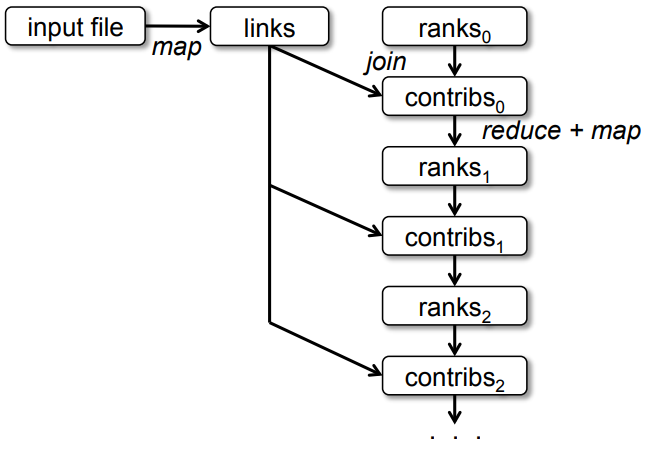
\includegraphics[scale=0.33]{imagens/lineage-graph-pagerank.png}
    \end{center}
    \small{Fonte: \cite{zaharia2012rdd}}
    \label{fig:lineage-pagerank}
\end{figure}

Analisando o grafo gerado na Figura \ref{fig:lineage-pagerank}, inicialmente é realizada a carga de um arquivo de entrada. A seguir, é aplicada uma função de \textit{map} para gerar o RDD contendo os \textit{links}. Durante a execução a aplicação, o RDD \textit{links} é frequentemente reutilizado na geração de novos RDDs com resultados intermediários. Como consequência, este RDD torna-se um candidato a ser armazenado em \textit{cache}, a fim de evitar sua recomputação a cada utilização e consequentemente reduzir o tempo de processamento da aplicação. Nesse exemplo, o RDD \textit{links} possui uma frequência de reutilização igual a 3, enquanto os demais RDDs do \textit{job} apresentam frequência igual a 1.


\subsection{Implementação}
Para realizar a implementação do Algoritmo Baseado em Prioridades, a primeira etapa do processo consiste na extração de métricas da aplicação a partir dos RDDs que serão utilizados no \textit{job}. Para tanto, parte-se do RDD cuja ação foi aplicada, até não encontrar novas dependências. Na sequência, navega-se, de forma recursiva, nas dependências do estágio gerado pelo \textit{DAGScheduler} para realizar o processamento do \textit{job}. 

Este processo é exemplificado através do método exibido no Algoritmo \ref{alg:lista-rdds}. Primeiro, adiciona-se o RDD visitado na lista de RDDs já processados (Linha 3) e em seguida, percorre-se cada dependência adicionada na lista de dependências do RDD visitado (Linhas 4--6). Por fim, se a dependência ainda não foi processada (Linha 5), repete-se este mesmo processo para a dependência em questão (Linha 6). O resultado desta primeira etapa consiste em uma lista contendo todos os RDDs que serão criados e manipulados durante a computação do \textit{job}. 

\begin{figure}[!ht]
    \begin{algorithm}[H]
        \caption{Identificação dos RDDs utilizados no \textit{job}.}
        \label{alg:lista-rdds}
        \Entrada{StageResult gerado pelo DAGScheduler.}
        \Saida{Lista com todos os RDDs identificados no \textit{job}.}
        rddsDependencies $\leftarrow$ List[RDD]\;
        
        \SetKwProg{Fn}{Function}{ is}{end}
        \Fn{getRddsUsedInJob(rdd: RDD[\_], rddsDependencies: List[RDD])}{
           rddsDependencies += rdd\;
           
           \ForEach{deps in rdd.dependencies}{
                \If{deps $\notin$ rddsDependencies}{
                    getRddsUsedInJob(deps, rddsDependencies)\;
                }
           }
        }
    \end{algorithm}
\end{figure}

Após a identificação dos RDDs, a próxima etapa consiste na coleta das métricas desejadas, as quais serão utilizadas no processo de gerência de memória. O processo de coleta utilizado é ilustrado pelos métodos apresentados nos Algoritmos \ref{alg:tamanho-lineage-rdds}, \ref{alg:frequencia-acesso-rdds} e \ref{alg:frequencia-reutilizacao-rdds}, cada qual responsável por obter uma determinada métrica.

\begin{figure}[!ht]
    \begin{algorithm}[H]
        \caption{Obtenção do Tamanho da \textit{Lineage}}
        \label{alg:tamanho-lineage-rdds}
        \Entrada{List[RDD] contendo os RDDs utilizados no job}
        \Saida{Estrutura HashMap contendo o id do RDD e seu respectivo tamanho da \textit{lineage}.}
        lineageSize $\leftarrow$ HashMap[RDD, Int]\;
        
        \SetKwProg{Fn}{Function}{}{end}
        \Fn{getLineageSize(rdd: RDD[\_], rddID: Int, list: HashMap[RDD, Int], visited: List[RDD])} {
           update(lineageSize[rddId])\; 
           
           \ForEach{deps in rdd.dependencies} {
                \If{deps $\notin$ visited} {
                    visited += deps\;
                    getLineageSize(deps, rddID, list, visited)\;
                }
           }
        }
    \end{algorithm}
\end{figure}

O método \textit{getLineageSize}, ilustrado pelo Algoritmo \ref{alg:tamanho-lineage-rdds}, visa obter o tamanho da \textit{Lineage} de um RDD. Para isto, atualiza-se o tamanho atual do RDD, iniciando em 0 (Linha 3). Em seguida, percorre-se as dependências desse RDD (Linhas 4--9) verificando se a dependência em questão ainda não foi processada (Linha 5). Caso a dependência não tenha sido processada, adiciona-se esta à lista de nodos visitados (Linha 6) e processa-se esta nova dependência (Linha 7). 

Nesta implementação é importante evitar que uma dependência seja visitada mais de uma vez, impedindo que um mesmo RDD seja contabilizado diversas vezes. O resultado desse método consiste em um mapa onde as chaves são os RDDs e o tamanho de suas \textit{lineages}. Este método deve ser chamado de forma individual para cada RDD manipulado no \textit{job}.

\begin{figure}[!ht]
    \begin{algorithm}[H]
        \caption{Obtenção da Frequência de Acesso}
        \label{alg:frequencia-acesso-rdds}
        \Entrada{List[RDD] contendo os RDDs utilizados no job}
        \Saida{Estruturas HashMap contendo o id do RDD e sua respectiva frequência de acesso.}
        frequencyAccess $\leftarrow$ HashMap[RDD, Int]\;
        
        \SetKwProg{Fn}{Function}{}{end}
        \Fn{getUseFrequency(rdd: RDD[\_], frequencyAccess: List[RDD])} {
           update(frequencyAccess[rdd])\;
           
           \ForEach{deps in rdd.dependencies} {
                getUseFrequency(deps, frequencyAccess)\;
           }
        }
    \end{algorithm}
\end{figure}

O método \textit{getUseFrequency}, denotado no Algoritmo \ref{alg:frequencia-acesso-rdds}, apresenta um comportamento semelhante ao método utilizado para contabilizar o tamanho da \textit{Lineage} (\textit{getLineageSize)}, mas com o objetivo de obter a frequência de Acesso de um RDD. Assim, primeiro atualiza-se a frequência do RDD, iniciando em 1 (Linha 3). Na sequência, percorre-se as dependências do RDD (Linhas 4--6), processando-as. 

Neste método não há necessidade de realizar o controle dos nodos visitados, uma vez que o RDD deve ser acessado para a computação de cada novo RDD gerado a partir deste. Ao final de sua execução, o resultado é uma estrutura mapeando cada RDD com sua respectiva quantidade de acesso.

\begin{figure}[!ht]
    \begin{algorithm}[H]
        \caption{Obtenção da Frequência de Reutilização}
        \label{alg:frequencia-reutilizacao-rdds}
        \Entrada{List[RDD] contendo os RDDs utilizados no job}
        \Saida{Estruturas HashMap contendo o id do RDD e sua respectiva frequência de reutilização.}
        reuseFrequency $\leftarrow$ HashMap[RDD, Int]\;
        
        \SetKwProg{Fn}{Function}{}{end}
        \Fn{getRDDsReuse(rddList: List[RDD], reuseFrequency: HashMap[RDD, Int])} {
           
           \ForEach{rdd in rddList} {
                dependencies $\leftarrow$  rdd.dependencies\;
                \ForEach{deps in dependencies} {
                    update(reuseFrequency[deps])\;
                }
           }
        }
    \end{algorithm}
\end{figure}

O método \textit{getRDDsReuse}, ilustrado pelo Algoritmo \ref{alg:frequencia-reutilizacao-rdds}, visa obter a frequência de reutilização de cada RDD manipulado. Esse processo é realizado de modo que, para cada RDD do \textit{job} (Linhas 3--8), percorre-se todas as dependências do RDD (Linhas 4--7) e agrega-se a quantidade de reutilização de cada RDD em tais dependências (Linha 6). Ao final do processamento, é gerado um mapa contendo como chave o RDD e como valor a sua respectiva frequência de reutilização.

Conforme demonstrado pelo Algoritmo \ref{alg:calculo-prioridade-rdds}, o método responsável calcular a prioridade de cada RDD visa iterar sobre todos os RDDs identificados previamente  (Linhas 5--11) e calcular sua respectiva prioridade. Este cálculo é realizado utilizando o tamanho da \textit{lineage} (Linha 6), a frequência de acesso (Linha 7) e a frequência de reutilização (Linha 8). O resultado deste cálculo consiste na prioridade do RDD (Linha 9), a qual será mantida em uma lista contendo todos os RDDs utilizados no \textit{job} (Linha 10) e posteriormente ordenados de maneira decrescente por prioridade (Linha 12).

Os RDDs com pontuações maiores, encontrados se nas posições iniciais da lista, deverão ter suas partições removidas o mais tarde possível. Deste modo, prioriza-se aqueles RDDs com maior frequência de reutilização em processamentos subsequentes a fim de eliminar a necessidade de recomputá-los a cada utilização.

\begin{figure}[!ht]
    \begin{algorithm}[H]
        \caption{Cálculo da Prioridade do RDD.}
        \label{alg:calculo-prioridade-rdds}
        \Entrada{Três HashMaps contendo as métricas extraídas do \textit{job}.}
        \Saida{Lista ordenada contendo a prioridade de cada RDD.}
        rdds $\leftarrow$ List[RDD]\;
        lineageSize, frequencyAccess, reuseFrequency $\leftarrow$ HashMap[RDD, Int]\;
        
        \SetKwProg{Fn}{Function}{}{end}
        \Fn{getRddsUsedInJob()} {
           priority $\leftarrow$ HashMap[RDD, Float]\;
           \ForEach{rdd in rdds}{
                size $\leftarrow$ lineageSize[rdd]\;
                access $\leftarrow$ frequencyAccess[rdd]\;
                reuse $\leftarrow$ reuseFrequency[rdd]\;
                
                value $\leftarrow$ reuse * (size * 0,5 + access * 0,5)\;
                priority.add(rdd, value)\;
           }
           
           return sort(priority)\;
        }
    \end{algorithm}
\end{figure}

Após a conclusão do processamento e do cálculo das prioridades dos RDDs do \textit{job}, o resultado final é armazenado no \textit{Driver} da aplicação. A difusão da lista com as prioridades de cada RDD é realizada entre os nodos do \textit{cluster} sob demanda. Isso significa que a comunicação entre um \textit{Executor}, hospedado pelos nodos \textit{Workers}, e o \textit{Driver} irá ocorrer apenas quando a memória desse \textit{Executor} estiver sobrecarregada e necessitando realizar a remoção de partições. 

Nessas situações de sobrecarga da memória, o Spark \textit{Executor} irá solicitar a lista contendo a prioridade de cada RDD do \textit{job}. Embora haja penalização no tempo de comunicação, esta requisição é realizada utilizando comunicação síncrona entre o \textit{Driver} e o \textit{Executor}. O sincronismo é necessário, uma vez que a lista com as prioridades é uma informação fundamental para realizar a ordenação das partições em memória e a remoção de dados.


A requisição de atualização da lista de prioridade ocorre em duas situações: quando a lista com as prioridades está vazia e quando o identificador de uma partição não é encontrado. A ausência de um identificador na lista indica que um novo \textit{job} iniciou e novos RDDs foram manipulados, necessitando que a lista de prioridades seja atualizada em cada \textit{Executor}. O \textit{status} de lista vazia significa que o processamento da aplicação começou recentemente e nenhum bloco foi removido. 


\subsection{Análise de Correlação} \label{subsec:analise-convergencia}
A fim de verificar a correlação da Equação \ref{eq:priorityCalculation}, proposta na Seção \ref{sec:alg-pesos}, realizou-se uma análise de correlação do método utilizado para calcular a prioridade de cada RDD. Esta é uma análise flexível, que pode ser usada sempre que uma variável quantitativa for estudada em função a qualquer fator de interesse \cite{cohen2014applied}. Esta análise tem como objetivo medir o grau de dependência entre duas variáveis, sendo indicada para avaliar a hipótese de que o aumento ou decréscimo em uma variável está associado ao comportamento de outra.

Através do coeficiente de Pearson \cite{benesty2009pearson}, responsável por representar a correlação entre as variáveis observadas, é possível medir o grau de relacionamento entre as variáveis. Este coeficiente, o qual é desprovido de unidade ou ordem de grandeza, assume valores entre -1 e 1. Valores maiores que 0 indicam uma correlação positiva, isto é, ambas as variáveis observadas movem-se na mesma direção e a relação é mais forte quando o resultado se aproxima de 1. De modo similar, valores menores que 0 indicam uma correlação negativa, ou seja, as variáveis movem-se em direções contrárias e essa correlação é mais forte quando o resultado se aproxima de -1. Por fim, um coeficiente igual a 0 indica que não há correlação entre as variáveis observadas.


Para realizar a análise de correlação da equação proposta (Equação \ref{eq:priorityCalculation}), desenvolveu-se uma aplicação Python\footnote{https://www.python.org/}, com o objetivo de simular o comportamento e a configuração de diferentes \textit{lineages} dentro de um \textit{job} no Spark. Esta aplicação é composta por três funções:

\begin{enumerate}
	\item[a)] Geração de uma \textit{lineage}: consiste em gerar diferentes combinações de \textit{lineages} possíveis dentro de um \textit{job};
	\item[b)] Obtenção das métricas desejadas: visa extrair, a partir da \textit{lineage}, as métricas referentes ao tamanho da \textit{lineage}, à frequência de acesso e à frequência de reutilização;
	\item[c)] Cálculo da prioridade de cada RDD extraído: objetiva criar uma lista de prioridades para cada combinação de tamanho da \textit{lineage}, frequência de acesso e frequência de reutilização gerada pela aplicação.
\end{enumerate}

A aplicação visa simular a extração de métricas de forma análoga ao implementado no Spark. Assim, a análise foi realizada utilizando \textit{lineages} com tamanho variando entre 5 e 60, onde, para cada configuração de tamanho, variou-se a frequência de reutilização entre 1\% e 70\% do tamanho da \textit{lineage}, totalizando 46,561 configurações para o cálculo da prioridade dos RDDs. Estas configurações de \textit{lineage} tinham como objetivo simular o comportamento de aplicações com diferentes quantidades de reutilização de RDDs.

Os resultados desta análise demonstram que existe uma forte correlação positiva entre a prioridade calculada e a frequência de reutilização, atingindo um coeficiente de correlação superior a 0,94. Quando examinamos as demais variáveis, ambas também apresentam uma correlação positiva com a prioridade calculada, com coeficientes iguais a 0,32 e 0,013 para a frequência de acesso e tamanho da \textit{lineage}, respectivamente. 

Conforme demonstrado pela análise de correlação realizada na equação proposta, o fator determinante para o crescimento da pontuação recebida pelo RDD é a frequência de reutilização, dada a sua alta correlação com o resultado da equação proposta. As demais métricas utilizadas apresentam pouca influência no resultado final geral, exercendo maior influência em situações onde a frequência de reutilização é igual para todos os RDDs.

Uma consequência desse algoritmo baseado em prioridades é um comportamento imprevisível em aplicações onde há uma mesma frequência de reutilização de vários RDDs. Em tais situações, o critério para diferenciar uma prioridade das demais será calculada baseando-se apenas na frequência de acesso e tamanho da \textit{lineage}. Ademais, a utilização de métricas auxiliares apresentam pouco impacto no resultado gerado, ao mesmo tempo que tornam a implementação do algoritmo proposto mais complexa.

\subsection{Experimentos e Resultados}
A validação do Algoritmo Baseado em Prioridades, apresentado na Seção \ref{sec:lru-mfu}, foi realizada através de experimentos em um \textit{cluster} distribuído. Os experimentos foram conduzidos na plataforma Grid'5000, utilizando um \textit{cluster} com 7 nodos, sendo a escolha desta configuração realizada tendo como base o tamanho do conjunto de dados utilizado nos experimentos. Assim, através desta configuração de \textit{cluster}, torna-se possível criar cenários com diferentes cargas de acesso a memória.

Os nodos selecionados foram configurados da seguinte maneira: 1 Spark \textit{Master}, 4 Spark \textit{Workers} hospedando 1 \textit{Executor} por nodo, 1 nodo executando o \textit{HDFS Namenode} e \textit{HDFS Datanode} e 1 nodo executando o \textit{HDFS Datanode}. Cada nodo do sistema era composto por dois Intel Xeon E5-2630 v3 @2.2GHz (8 \textit{cores}/CPU), 128GB de memória RAM e dois HDs de 558GB, conectados via \textit{ethernet} 10Gbps. O sistema operacional utilizado foi o Debian 8, juntamente com Java JDK 1.8.202, Spark 2.2.0 e Hadoop 2.7.1. 

% [corrigido]
Para os experimentos, utilizou-se os algoritmos \textit{PageRank}, \textit{K-Means} e \textit{Logistic Regression} como \textit{benchmarks}, sendo estes implementados pelo Intel HiBench \cite{huang2010hibench}. O \textit{benchmark Logistic Regression} consiste em um tipo de análise estatística utilizada frequentemente para análise preditiva. A inclusão deste \textit{benchmark} tem como objetivo obter uma melhor amostra de aplicações com diferentes tamanhos e disposições das \textit{lineages}. Ainda, foram utilizados dois tamanhos de \textit{datasets}: \textit{small} e \textit{large}. A Tabela \ref{tab:tamanho-datasets} apresenta o tamanho destes \textit{datasets} em cada \textit{benchmark}.

\begin{table}[!ht]
    \centering
        \caption{Tamanho dos Datasets utilizados}
        \label{tab:tamanho-datasets}
            \begin{tabular}{cccc}
                \hline
                Tamanho & PageRank & K-Means & Logistic Regression \\ \hline
                Small & 1,7 MB & 574,6 MB & 76,4 MB \\
                Large & 247,9 MB & 3,7 GB & 7,5 GB \\ \hline
        \end{tabular}
\end{table}

Além da variação no tamanho dos \textit{datasets} utilizados, cada Spark \textit{Executor} teve a sua memória variando entre 4 configurações distintas: 1 GB, 1,5 GB, 2 GB e 4 GB. É importante ressaltar que estas configurações representam a memória total disponibilizada para o \textit{Executor}, ou seja, incluem a Memória de Armazenamento, a Memória de Execução e a Memória do Usuário.

O espaço dedicado ao armazenamento de informações corresponde a uma fração da quantidade total de memória disponível. Deste modo, na Tabela \ref{tab:memoria-algo-prioridades} são demonstrados três valores de memória: Memória Total, Memória de Armazenamento e Memória Total de Armazenamento Disponível. A Memória Total descreve ao espaço total disponível para ser dividido entre as 3 regiões de memória do Spark (Memória de Execução, Memória de Armazenamento e Memória do Usuário). A Memória de Armazenamento se refere à fração de memória destinada ao armazenamento dos dados no \textit{Executor}, ou seja, o espaço disponível para manter dados em \textit{cache}. Por fim, a Memória Total de Armazenamento Disponível denota o somatório da Memória de Armazenamento de todos os \textit{Executors} do \textit{cluster}, simbolizando o espaço máximo para realizar o armazenamento dos dados.

\begin{table}[!ht]
    \caption{Configuração de Memória Utilizada - Algoritmo Baseado em Prioridades}
    \label{tab:memoria-algo-prioridades}
    \centering
    \scalebox{0.9}{
    \begin{tabular}{ccc}
        \hline
        Memória Total & Memória de Armazenamento & Memória Total de Armazenamento Disponível \\ \hline
        1 GB & 366,3 MB & 1465,2 MB \\
        1.5 GB & 639,3 MB & 2557,2 MB \\
        2 GB & 912,3 MB & 3649,2 MB \\
        4 GB & 2004,4 MB & 8018,4 MB \\ \hline
    \end{tabular}
    }
\end{table}

As variações na quantidade de memória utilizada, bem como no tamanhos dos \textit{datasets}, têm como objetivo avaliar O Algoritmo Baseado em Prioridades sob duas condições. A primeira condição é em situações onde a memória disponível é suficiente para comportar o \textit{dataset}. A segunda, em situações de sobrecarga exigindo que seja feita a substituição de partições em memória. Os resultados obtidos na experimentação representam os tempos de execução dos \textit{benchmarks} utilizando o Algoritmo Baseado em Prioridades em contraponto ao LRU nativamente implementado pelo Spark. Assim, estes resultados são a média aritmética de 20 execuções dos \textit{benchmarks} em cada configuração.

Os resultados demonstrados na Tabela \ref{tab:algo-prioridade-resultado-small} e na Figura \ref{fig:algo-prioridade-resultado-small} referem-se à utilização de um \textit{dataset small}. Já a Tabela \ref{tab:algo-prioridade-resultado-large} e a Figura  \ref{fig:algo-prioridade-resultado-large} exibem os resultados obtidos com um \textit{dataset large}. Quando analisamos os resultados obtidos com o \textit{dataset small}, durante a execução do \textit{benchmark K-Means} houve necessidade de realizar a substituição de partições da memória. Esta necessidade pode ser verificada através dos \textit{logs} de execução dos \textit{benchmarks}. Nestes casos, o Algoritmo por Prioridades foi 40,74\% e 23,5\% mais rápido quando comparado com o LRU com as configurações de 1 GB e 1,5 GB, conforme demonstrado pela Figura \ref{fig:algo-prioridade-resultado-small}(a). Quando há espaço disponível para todo o conjunto de dados, o desempenho de ambos os algoritmos é equivalente, uma vez que nenhuma partição foi removida da memória. Estas situações podem ser observadas nas Figuras \ref{fig:algo-prioridade-resultado-small}(b) e \ref{fig:algo-prioridade-resultado-small}(c), apresentando um tempo de execução similar nesta configuração.



\begin{table}[!ht]
    \caption{Tempos de Execução dos Benchmarks: \textit{Dataset small}}
    \label{tab:algo-prioridade-resultado-small}
    \centering
    \scalebox{0.9}{
    \begin{tabular}{ccccc}
        \hline
        Benchmark & Algoritmo & \begin{tabular}[c]{@{}c@{}}Memória \\ Disponível\end{tabular} & \begin{tabular}[c]{@{}c@{}}Tempo de \\ Execução (em s)\end{tabular} & \begin{tabular}[c]{@{}c@{}}Desvio \\ Padrão (em s)\end{tabular} \\ \hline
        \multirow{6}{*}{Pagerank} & LRU & 1G & 7,95 & 0,19 \\
         & Prioridades & 1 GB & 8,27 & 0,31 \\ \cline{2-5} 
         & LRU & 1,5 GB & 7,98 & 0,32 \\
         & Prioridades & 1,5 GB & 8,11 & 0,36 \\ \cline{2-5} 
         & LRU & 2 GB & 7,95 & 0,34 \\
         & Prioridades & 2 GB & 8,16 & 0,40 \\ \hline
        \multirow{6}{*}{K-Means} & LRU & 1 GB & 29,16 & 4,94 \\
         & Prioridades & 1 GB & 17,28 & 0,69 \\ \cline{2-5} 
         & LRU & 1,5 GB & 22,72 & 2,10 \\
         & Prioridades & 1,5 GB & 17,38 & 0,46 \\ \cline{2-5} 
         & LRU & 2 GB & 15,14 & 0,42 \\
         & Prioridades & 2 GB & 15,55 & 0,63 \\ \hline
        \multirow{6}{*}{LR} & LRU & 1 GB & 16,94 & 0,56 \\
         & Prioridades & 1 GB & 16,51 & 0,19 \\ \cline{2-5} 
         & LRU & 1,5 GB & 16,64 & 0,18 \\
         & Prioridades & 1,5 GB & 16,57 & 0,21 \\ \cline{2-5} 
         & LRU & 2 GB & 16,73 & 0,30 \\
         & Prioridades & 2 GB & 16,59 & 0,18 \\ \hline
    \end{tabular}
    }
\end{table}



\begin{figure}[!ht]
    \centering
    \caption{Tempos de Execução dos Benchmarks: Dataset Small}
    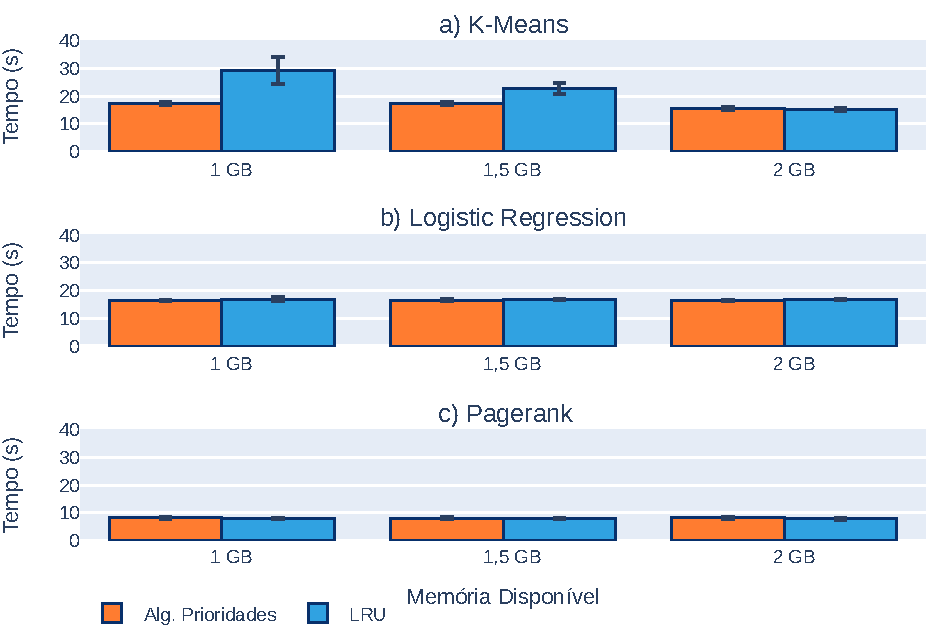
\includegraphics[scale=0.85]{imagens/resultados-dateset-small.pdf}
    \label{fig:algo-prioridade-resultado-small}
\end{figure}

Conforme exibem a Tabela \ref{tab:algo-prioridade-resultado-large} e a Figura \ref{fig:algo-prioridade-resultado-large}, quando analisamos os dados com um \textit{dataset} maior, os resultados obtidos demonstram que o Algoritmo Baseado em Prioridades, em média, pode apresentar um desempenho igual ou superior ao LRU nas mesmas condições. Examinando os resultados do \textit{benchmark K-Means} (Figura \ref{fig:algo-prioridade-resultado-large}(a)), constata-se que ambos algoritmos apresentaram desempenho equivalente em todas as configurações. Uma análise dos \textit{logs} gerados por essa aplicação revela que a memória comporta todo o \textit{dataset}, quando utilizadas as configurações de 2 GB e 4 GB. Nas configurações de 1 GB e 1,5 GB, a memória encontra-se fortemente sobrecarregada, uma vez que o \textit{dataset} ocupa todo o espaço disponível. Nesses casos, partições de dados serão descarregadas da memória de forma inevitável, a fim de liberar espaço para armazenamento de novos dados.


\begin{table}[!ht]
    \caption{Tempos de Execução do Algoritmo utilizando o \textit{Dataset large}}
    \label{tab:algo-prioridade-resultado-large}
    \centering
    \scalebox{0.90}{
    \begin{tabular}{ccccc}
        \hline
        Benchmark & Algoritmo & \begin{tabular}[c]{@{}c@{}}Memória \\ Disponível\end{tabular} & \begin{tabular}[c]{@{}c@{}}Tempo de \\ Execução (em s)\end{tabular} & \begin{tabular}[c]{@{}c@{}}Desvio \\ Padrão (em s)\end{tabular} \\ \hline
        \multirow{8}{*}{Pagerank} & LRU & \multirow{2}{*}{1 GB} & 156,40 & 36,92 \\
         & Prioridades &  & 150,11 & 21,51 \\ \cline{2-5} 
         & LRU & \multirow{2}{*}{1,5 GB} & 222,76 & 73,78 \\
         & Prioridades &  & 194,79 & 59,55 \\ \cline{2-5} 
         & LRU & \multirow{2}{*}{2 GB} & 64,90 & 2,46 \\
         & Prioridades &  & 65,09 & 1,98 \\ \cline{2-5} 
         & LRU & \multirow{2}{*}{4 GB} & 59,54 & 2,55 \\
         & Prioridades &  & 59,69 & 2,53 \\ \hline
        \multirow{8}{*}{K-Means} & LRU & \multirow{2}{*}{1 GB} & 454,72 & 11,69 \\
         & Prioridades &  & 450,19 & 13,44 \\ \cline{2-5} 
         & LRU & \multirow{2}{*}{1,5 GB} & 317,09 & 7,94 \\
         & Prioridades &  & 315,76 & 10,28 \\ \cline{2-5} 
         & LRU & \multirow{2}{*}{2 GB} & 149,64 & 6,33 \\
         & Prioridades &  & 148,47 & 4,79 \\ \cline{2-5} 
         & LRU & \multirow{2}{*}{4 GB} & 40,02 & 2,07 \\
         & Prioridades &  & 39,85 & 1,58 \\ \hline
        \multirow{8}{*}{LR} & LRU & \multirow{2}{*}{1 GB} & 0 & 0 \\
         & Prioridades &  & 0 & 0 \\ \cline{2-5} 
         & LRU & \multirow{2}{*}{1,5 GB} & 0 & 0 \\
         & Prioridades &  & 0 & 0 \\ \cline{2-5} 
         & LRU & \multirow{2}{*}{2 GB} & 1180,35 & 25,72 \\
         & Prioridades &  & 1048,58 & 14,01 \\ \cline{2-5} 
         & LRU & \multirow{2}{*}{4 GB} & 278,59 & 11,84 \\
         & Prioridades &  & 264,68 & 11,09 \\ \hline
    \end{tabular}
    }
\end{table}

Devido a restrições de disponibilidade de memória, ambos os algoritmos não conseguiram executar o \textit{Benchmark Logistic Regression} nas configurações com 1 GB e 1,5 GB disponíveis, conforme ilustram a Tabela \ref{tab:algo-prioridade-resultado-large}
e a Figura  \ref{fig:algo-prioridade-resultado-large}(b). Investigando os \textit{logs} de execução do \textit{Logistic Regression}, verificou-se que todas as execuções foram interrompidas devido a uma exceção do tipo \textit{OutOfMemoryError}. Esta exceção ocorre quando a JVM gasta uma grande quantidade de tempo executando a rotina de remoção de memória do \textit{Garbage Collector}, provocado pela exaustão da memória disponível. Na configuração com configuração de 2 GB de memória, o Algoritmo Baseado em Prioridades reduziu em 11,16\% o tempo de execução desta aplicação quando comparado ao comparado ao LRU. Por fim, utilizando 4 GB, o Algoritmo Baseado em prioridades foi 4,99\% mais rápido que o LRU nas mesmas condições.


\begin{figure}[!ht]
    \centering
    \caption{Tempos de Execução dos Benchmarks: Dataset Large}
    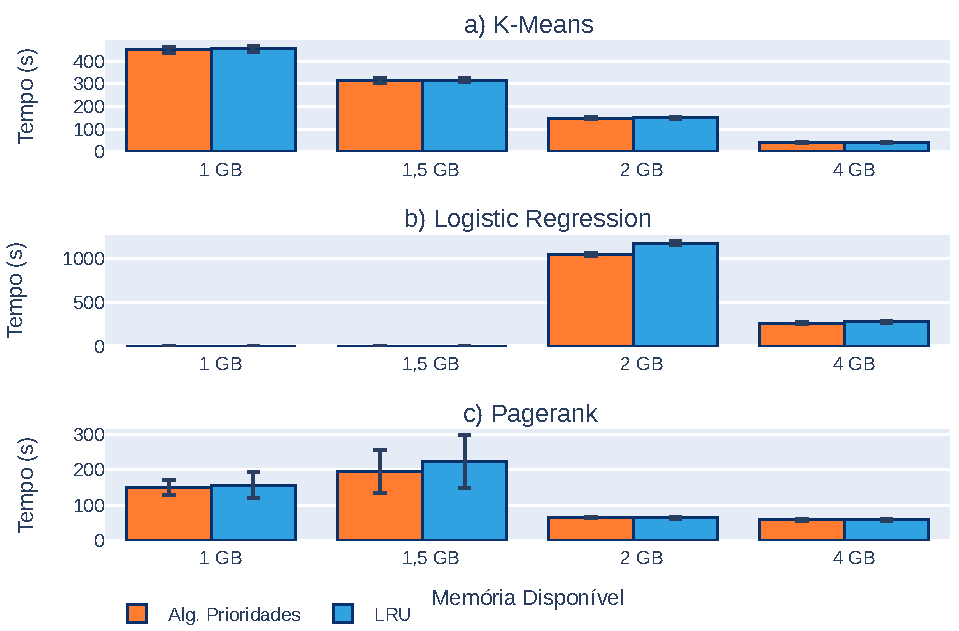
\includegraphics[scale=0.85]{imagens/resultados-dateset-large.pdf}
    \label{fig:algo-prioridade-resultado-large}
\end{figure}

Com o \textit{benchmark Pagerank} (Figura \ref{fig:algo-prioridade-resultado-large}(c)), o Algoritmo por Prioridades foi 5,3\% mais rápido na configuração com configuração de 1GB, e 12,56\% mais rápido quando há 1,5 GB disponíveis, se comparados ao LRU nas mesmas condições. Semelhante ao ocorrido quando utilizado a configuração com \textit{dataset} menor, nas configurações com 2 GB e 4 GB o desempenho foi equivalente, uma  vez que foi possível manter todos os dados em memória e, consequentemente, não houve necessidade de substituições de partições da memória.


\section{Gerenciamento Dinâmico da Memória} \label{sec:gerenc-dinamico}
A utilização de métricas obtidas da aplicação em execução pode trazer bons resultados, diminuindo o tempo necessário para realizar o processamento da mesma, especialmente em cenários onde há reutilização de de dados. Entretanto, analisando o funcionamento do LRU implementado nativamente pelo Spark, percebe-se que essa solução funciona de maneira reativa. Isto significa que é executada em situações onde o Spark detecta a inexistência de espaço disponível para armazenamento de novas informações. 

Na implementação do LRU nativa no Spark, após a detecção da indisponibilidade de espaço, as rotinas de gerenciamento de memória são executadas com o objetivo de remover a quantidade de dados suficientemente grande para comportar os novos dados da memória. Por consequência, a execução da aplicação é interrompida e postergada até que as rotinas de remoção de blocos da memória sejam completamente executadas.

Este trabalho implementa um modelo de Gerenciamento Dinâmico da Memória para aplicações onde há reutilização de dados. O modelo visa monitorar a aplicação em execução a fim de identificar, de forma antecipada, a necessidade de realizar a remoção de blocos de memória. Através desta abordagem, busca-se diminuir a sobrecarga das operações de substituição de blocos da memória.

A implementação do Gerenciamento Dinâmico é divida em dois componentes: um algoritmo de substituição de blocos da memória e um agente externo. O algoritmo tem como objetivo estabelecer um critério, baseando-se em informações extraídas da aplicação em execução, para decidir qual bloco deve ser removido da memória. Para tanto, este algoritmo visa agregar a Frequência de Reutilização dos RDDs utilizados no \textit{job} juntamente com o algoritmo LRU.

O algoritmo utilizado no Gerenciamento Dinâmico consiste em uma otimização do LRU, sendo este uma evolução do algoritmo apresentado na Seção \ref{sec:alg-pesos}, com o objetivo de priorizar RDDs com reutilização dentro do \textit{job}. Para tanto, descarta-se as métricas com baixa relevância, ou seja, a Frequência de Acesso e Tamanho da \textit{Lineage}, identificadas na análise de correlação (Seção \ref{subsec:analise-convergencia}), fazendo uso apenas da Frequência de Reutilização. 

O algoritmo implementado no modelo de gerenciamento mantém uma lista ordenada pela Frequência de Reutilização dos RDDs identificados no \textit{job} e, em caso de empate, utiliza-se o algoritmo LRU para realizar a sub-ordenação dessas partições. Deste modo, em situações onde não há reutilização de RDDs, o comportamento do algoritmo será semelhante ao LRU implementado nativamente pelo Spark.

O Agente Externo visa obter métricas, sendo estas o consumo de memória, a quantidade de estágios de um \textit{job} e o \textit{status} da execução destes estágios, através da API REST do Spark. A partir dessas métricas, busca-se antecipar a necessidade de espaço livre em memória. Assim, pode-se executar rotinas de remoção de blocos da memória em segundo plano, de modo a reduzir a sobrecarga causada por tais operações.

O modelo de Gerenciamento da Memória implementado, exibido na Figura \ref{fig:arquitetura-dinamica}, é composto por:
\begin{enumerate}
	\item[a)] 1 nodo \textit{Spark Master}, responsável por gerenciar os contextos das aplicações;
	\item[b)] $n$ nodos \textit{Spark Workers}, os quais possibilitam a escalabilidade do \textit{cluster} Spark;
	\item[c)] o \textit{Agente Observador}, cuja função é monitorar a aplicação;
	\item[d)] 1 nodo ZooKeeper, a fim de viabilizar a comunicação entre o Agente Observador e os nodos \textit{Spark Workers}.
\end{enumerate}

\begin{figure}[!ht]
    \caption{Modelo de Gerenciamento Dinâmico de Memória.}
    \begin{center}
        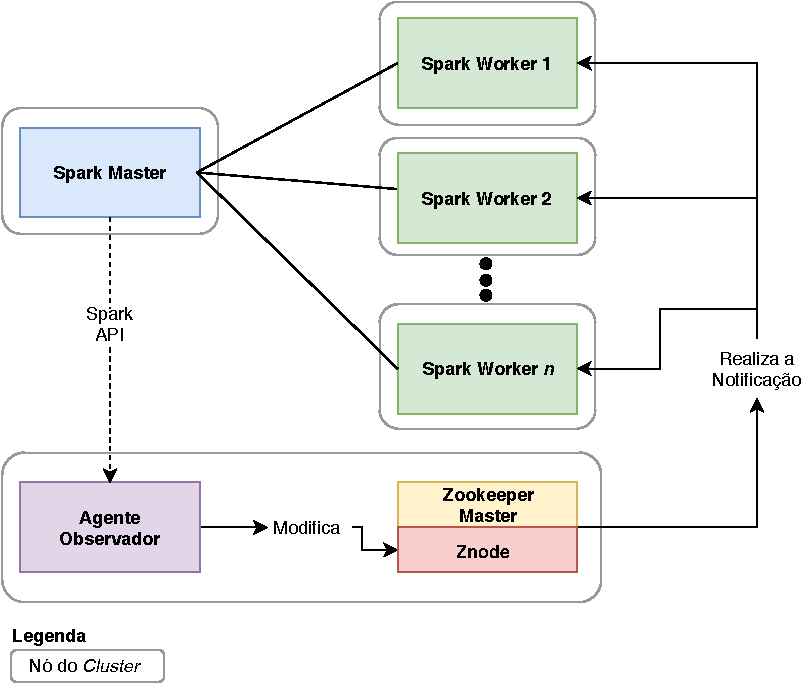
\includegraphics[scale=0.9]{imagens/arquitetura-dinamica.pdf}
    \end{center}
    \small{Fonte: Próprio autor}
    \label{fig:arquitetura-dinamica}
\end{figure}

No modelo de Gerenciamento Dinâmico da Memória, o \textit{Spark Master} é nodo responsável por hospedar o \textit{driver} da aplicação, juntamente com o seu contexto. Além disso, cabe ao \textit{Spark Master} gerenciar e distribuir tarefas para os nodos \textit{Workers} de modo a executar a aplicação. Durante a realização das computações requeridas pela aplicação, o \textit{Master} disponibiliza a sua API REST, onde o usuário pode efetuar requisições com o objetivo de instrumentar e obter estatísticas relacionas à execução. Através destas requisições, pode-se identificar as aplicações executando no \textit{cluster}, o \textit{status} da execução destas apliações, os RDDs armazenados em \textit{cache} e o consumo das memórias de armazenamento e execução.

O nodo ZooKeeper tem como objetivo prover os serviços deste \textit{framework}, permtindo a sincronização e a troca de mensagens entre o \textit{Agente Observador} e os nodos \textit{Workers} do Spark. Deste modo, foi disposto em apenas um nodo do \textit{cluster}, de maneira \textit{standalone}. O nodo ZooKeeper armazena, em memória, as estruturas dos \textit{znodes} utilizados para implementação do Gerenciamento Dinâmico. Assim, quando uma notificação a um determinado \textit{Worker} deve ser enviada, essas estruturas são manipuladas.

O \textit{Agente Observador} consiste em uma aplicação Java, responsável por realizar a conexão na API do Spark e efetuar o consumo dos dados, permitindo que sejam obtidas informações relativas ao estado atual das aplicações em execução. Por padrão, para cada \textit{Job}, são coletadas informações sobre o consumo de Memória de Armazenamento e de Execução, os estágios disponíveis juntamente com seus respectivos \textit{status} e a fração armazenada em memória do RDD em \textit{cache}.

A partir das informações coletadas, o \textit{Agente} busca estimar o melhor momento para realizar a liberação de memória no Spark. Para tanto, duas métricas são adotadas: o \textit{threshold} de ocupação de memória e o número de estágios pendentes.

O \textit{threshold} visa definir um limite máximo para a ocupação da memória, inferior a 100\%, de modo a manter uma determinada quantidade de memória livre. Assim, em situações onde novos dados devem ser armazenados em memória ou a Memória de Execução necessita de espaço extra para continuar a execução da \textit{task}, evita-se a necessidade de interromper a execução da aplicação para realizar a remoção do espaço requerido. 

Durante a execução da aplicação, caso o limite de ocupação da memória seja ultrapassado, pode haver a necessidade de remover blocos da memória. A remoção de dados é feita a fim de garantir uma fração da Memória de Armazenamento sempre disponível para a aplicação.

Uma segunda métrica utilizada consiste no \textit{status} dos estágios criados para o processamento do \textit{job} da aplicação. Em situações onde o \textit{threshold} foi atingido e foram identificados estágios pendentes para serem executados, partições devem ser removidas da memória a fim de liberar espaço.

Em contraponto, se a ocupação da memória atingir o limiar e não houver estágios pendentes, nenhuma ação é tomada. Deste modo, permite-se que a memória seja completamente ocupada, uma vez que não é possível identificar de forma antecipada se a execução de um novo \textit{job} será realizada.

Uma vez decididas quais partições devem ser removidas da memória, o Agente de Monitoramento deve realizar a notificação aos Spark \textit{Workers} para que estes iniciem as rotinas de remoção de blocos da memória. Para tanto, o Agente calcula, de forma individual, a quantidade de memória que cada \textit{Executor} deve liberar para ficar abaixo do \textit{threshold} estabelecido. Na sequência, o Agente escreve esta informação no \textit{znode} associado ao respectivo \textit{Executor}. 


\subsection{Implementação do Gerenciamento Dinâmico}
O desenvolvimento do modelo de Gerenciamento Dinâmico foi divido em três etapas de implementação: Algoritmo de gerenciamento de memória no Spark, Comunicação entre o Spark e o ZooKeeper e Agente de Monitoramento para instrumentação da aplicação.

\subsubsection{Algoritmo de Gerenciamento de Memória}
O algoritmo utilizado no modelo de Gerenciamento Dinâmico consiste em uma otimização do algoritmo LRU implementado nativamente pelo Spark. Este algoritmo une a localidade temporal do LRU juntamente com a Frequência de Reutilização dos RDDs para definir a ordem em que as partições serão removidas da memória. Uma vez que este algoritmo necessita de informações providas pela aplicação, torna-se necessário analisar a aplicação antes de efetivamente executá-la.

A extração das informações requeridas pelo algoritmo é realizada modificando o escalonador de \textit{jobs} do Spark, isto é, o \textit{DAGScheduler}. Após uma ação ser aplicada ao RDD, este é submetido ao escalonador do Spark para que seu plano de execução seja gerado, possibilitando a execução do \textit{job} no \textit{cluster}. Entretanto, antes de iniciar a execução das \textit{tasks} do \textit{job}, dois métodos são executados: \textit{getLineageGraphFromJob} e \textit{getRddsReuseFrequency}.

O método \textit{getLineageGraphFromJob}, exibido no Algoritmo \ref{fig:metodo-getLineageGraph}, é responsável por obter o grafo de dependências do \textit{job} a ser executado. Para isto, primeiro o RDD é adicionado na lista de nodos já computados (Linha 4), a fim de evitar que este RDD seja processado mais de uma vez. Em seguida, é gerada uma lista contendo todos os identificadores das dependências desse RDD (Linhas 5--8). Por fim, é realizado o mapeamento deste RDD junto com sua lista de dependências (Linha 9). Este procedimento é repetido para todas as dependências ainda não processadas do RDD (Linhas 10--14). Ao final deste método, a estrutura \textit{lineage} (Linha 2) armazenará os \textit{ids} dos RDDs juntamente com suas respectivas listas de dependências.


% \begin{figure}[!ht]
%     \caption{Método para Obtenção do Grafo de Dependências do \textit{Job}.}
%     \begin{center}
%         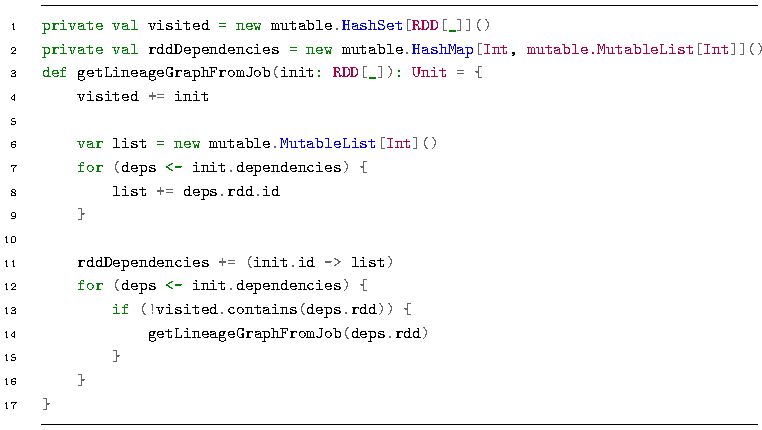
\includegraphics[scale=1.20]{imagens/metodo-getLineageGraph.pdf}
%     \end{center}
%     \small{Fonte: Próprio autor}
%     \label{fig:metodo-getLineageGraph}
% \end{figure}

% [corrigido]
\begin{figure}[!ht]
    \begin{algorithm}[H]
    \label{fig:metodo-getLineageGraph}
    \caption{Obtenção do Grafo de Dependências do \textit{Job}.}
        \Saida{Estrutura HashMap contendo os RDDs manipulados no \textit{job}.}
        
        \BlankLine
        visited $\leftarrow$ List[RDD]\;
        lineage $\leftarrow$ HashMap[Int, List[Int]]\;
        
        \BlankLine
        \SetKwProg{Fn}{Function}{}{end}
        \Fn{getLineageGraphFromJob(init: RDD[\_])} {
           add(init, visited)\;
           
           \BlankLine
           rddDependencies $\leftarrow$ List[Int]\;
           \ForEach{dep in init.dependencies} {
                add(dep.id, rddDependencies)\;
           }
           
           \BlankLine
           add([init.id, rddDependencies], lineage)\;
           \ForEach{dep in init.dependencies} {
                \If{dep $\notin$ visited} {
                    getLineageGraphFromJob(dep)\;
                }
           }
        }
    \end{algorithm}
\end{figure}


Após a obtenção do grafo de dependência, um segundo método é executado, visando gerar a frequência de reutilização de cada RDD mapeado. Esse método, denominado \textit{getRddsReuseFrequency}, é apresentado no Algoritmo \ref{fig:metodo-getReuseFrequency}. O objetivo do método  \textit{getRddsReuseFrequency} é acessar os RDDs identificados no \textit{job} (Linhas 2--12), acessando a lista de dependências de cada RDD (Linha 3). Em seguida, percorre-se a lista de dependências do RDD (Linhas 4--10), contabilizando a frequência em que cada RDD aparece na lista de dependências (Linhas 5--9). Deste modo, gera-se um mapa onde a chave consiste no identificador do RDD e o valor na Frequência de Reutilização.

% \begin{figure}[!ht]
%     \caption{Método para Obtenção da Frequência de Reutilização do RDD.}
%     \begin{center}
%         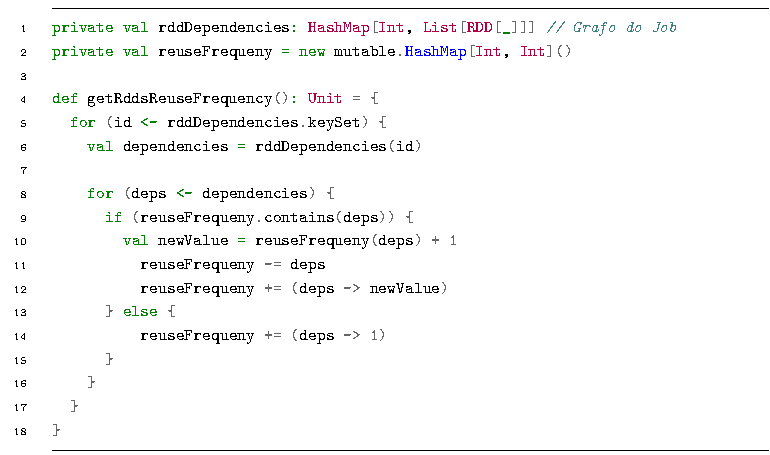
\includegraphics[scale=1.20]{imagens/metodo-getReuseFrequency.pdf}
%     \end{center}
%     \small{Fonte: Próprio autor}
%     \label{fig:metodo-getReuseFrequency}
% \end{figure}

% [corrigido]
\begin{figure}[!ht]
    \begin{algorithm}[H]
    \caption{Método para Obtenção da Frequência de Reutilização do RDD.}
        \label{fig:metodo-getReuseFrequency}
            \Entrada{lineage $\leftarrow$ HashMap[Int, List[RDD]] com o grafo de dependências}
            \Saida{reuseFrequency $\leftarrow$ HashMap[Int, Int] com a frequência de reutilização de cada RDD}
            
            \SetKwProg{Fn}{Function}{}{end}
            \BlankLine
            \Fn{getRddsReuseFrequency()}{
                \ForEach{rdd in lineage}{
                    dependencies $\leftarrow$ rdd.dependencies\;
                    \ForEach{deps in dependencies}{
                        \uIf{deps $\in$ dependencies}{
                            updateValue(deps, reuseFrequency, +1)\;
                        }
                        \Else{
                            add(deps, reuseFrequency)\;
                        }
                    }
                }
            }
    \end{algorithm}
\end{figure}

Uma vez realizado o processamento dos métodos \textit{getLineageGraphFromJob} e \textit{getRddsReuseFrequency}, o resultado gerado é mantido no \textit{Driver}, estando disponível para os \textit{Executors} da aplicação. O armazenamento dessas informações é feito através de um objeto do tipo  \textit{ShouldBeInCache}. A definição desta classe é ilustrada no Algoritmo \ref{fig:classe-shouldbeincache}, demonstrando seus principais métodos.

% \begin{figure}[!ht]
%     \caption{Armazenamento das Informações Processadas.}
%     \begin{center}
%         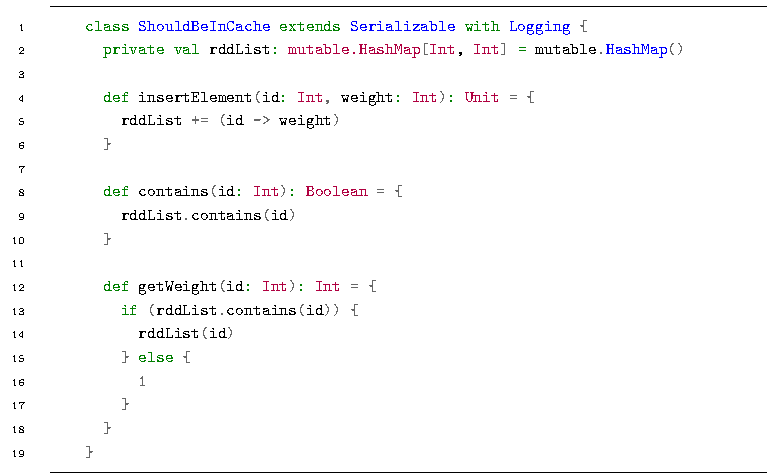
\includegraphics[scale=1.20]{imagens/classe-shouldbeincache.pdf}
%     \end{center}
%     \small{Fonte: Próprio autor}
%     \label{fig:classe-shouldbeincache}
% \end{figure}

% [corrigido]
\begin{figure}[!ht]
    \begin{algorithm}[H]
    \caption{Armazenamento das Informações Processadas.}
        \label{fig:classe-shouldbeincache}
            \SetKwProg{Fn}{Function}{}{end}
            \SetKwProg{Cs}{Class}{}{end}
            
            \Cs{ShouldBeInCache:} {
                rddList $\leftarrow$ HashMap[Int, Int]\; 
                
                \Fn{insertElemet(id: Int, score: Int)}{
                    add([id, score], rddList)\;
                }
                
                \BlankLine
                \Fn{contains(id: Int)}{
                    \textbf{return} id $\in$ rddList\;
                }
                
                \BlankLine
                \Fn{getReuseFrequency(id: Int)}{
                    \textbf{return} rddList[id]\;
                }
            }
    \end{algorithm}
\end{figure}

Conforme exibe o Algoritmo \ref{fig:classe-shouldbeincache}, a classe \textit{ShouldBeInCache} é responsável pelo armazenamento das informações obtidas do \textit{job}. O armazenamento dessas informações é realizado utilizando uma estrutura de \textit{HashMap} contendo identificador de RDD a uma respectiva Frequência de Reutilização (Linha 2). A inserção de dados é realizada através do método \textit{insertElement} (Linhas 3--5), a qual recebe o identificador do RDD e seu respectivo peso e adiciona ao \textit{HashMap} (Linha 4). O método \textit{contains} (Linhas 6--8) verifica se um RDD cujo identificador foi passada como parâmetro está armazenado no \textit{HashMap}. Por fim, o método \textit{getReuseFrequency} (Linhas 9--11) visa obter a Frequência de Reutilização de um RDD do RDD com identificador informado parâmetro. Se o identificar não for encontrado, esse método retorna 1. Isso ocorre para tratar os casos onde tenta-se verificar a Frequência de Reutilização de uma partição a qual não pertence a um RDD.

A definição da classe \textit{ShouldBeInCache} deve estender duas interfaces: \textit{Serializable} e \textit{Loggin}. A interface \textit{Serializable} visa permitir a transmissão de uma instância desse objeto através de chamadas RPC (\textit{Remote Procedure Call}), sendo este o método utilizado para realizar a comunicação entre nodos do Spark. A interface \textit{Logging} possibilita que sejam inseridas mensagens nos \textit{logs} de execução do Spark.

Após o processamento dos métodos implementados, a execução do \textit{job} é realizada sem quaisquer alterações. Deste modo, o Spark divide os estágios em \textit{tasks} e as executa nos \textit{Executors}. Durante a realização das computações requeridas pelos estágios, a memória pode ser esgotada e blocos de dados devem ser removidos da memória a fim de completar sua execução. 

A rotina de remoção de partições da memória deve priorizar a manutenção de blocos com a maior Frequência de Reutilização postergando, quando possível, a remoção destes blocos. Assim, primeiro deve-se remover blocos com menor Frequência de Reutilização e, para tanto, ordena-se os blocos mantidos em memória utilizando esta métrica. 

Para realizar a ordenação dos blocos de memória é necessário obter a lista atualizada das Frequências de Reutilização de cada RDD manipulado no \textit{job}. A fim de obter esta lista, o Spark \textit{Executor} envia uma solicitação ao \textit{Driver} da aplicação, requerendo a lista contendo as Frequências de Reutilização extraídas através do \textit{DAGScheduler}. Essa solicitação é enviada sempre que, durante a rotina de remoção de dados da memória, um RDD não for encontrado na lista armazenada pelo \textit{Executor}.

O cenário descrito indica que um novo \textit{job} foi iniciado e, portanto, a lista com a frequência de reutilização deve ser atualizada. Durante a atualização desta lista, a execução da rotina de remoção de blocos da memória é bloqueada até que o \textit{Executor} receba a resposta da chamada RPC realizada ao \textit{Driver}, garantindo o sincronismo da comunicação. Este sincronismo faz-se necessário, uma vez que as informações relativas a Frequência de Reutilização dos RDDs são indispensáveis para o prosseguimento da execução da rotina de remoção de partições da memória. Como consequência dessa comunicação síncrona, a execução da \textit{task} da aplicação é bloqueada até a conclusão da rotina de remoção de dados da memória.

Porém, a classe responsável por abrigar os métodos de gerenciamento de memória do Spark, denominada \textit{MemoryStore}, não tem acesso ao ambiente encarregado pela comunicação entre os nodos do \textit{cluster}. O acesso ao ambiente RPC pode ser realizado através do \textit{BlockManager}, responsável pelo armazenamento local e remoto de blocos de dados. 

Para possibilitar que os métodos de gerenciamento de memória tenham acesso ao ambiente de comunicação RPC, transmite-se uma referência do \textit{BlockManager} ao \textit{MemoryStore} após a sua criação, através de um método \textit{set} criado no \textit{MemoryStore}. Deste modo, as rotinas de gerenciamento de memória passam a ter acesso ao ambiente de comunicação e, consequentemente, torna-se possível realizar chamadas remotas diretamente destas rotinas. 

Assim, quando houver a necessidade de realizar a remoção de blocos de memória, realiza-se uma chamada direta ao \textit{Driver}, partindo do \textit{MemoryStore}, a fim de requerer a lista de Frequência de Reutilização obtida durante a análise do \textit{job}, visando ordenar as partições armazenadas de acordo com sua respectiva Frequência e Reutilização.

\subsubsection{Comunicação e Notificação Utilizando o ZooKeeper}
A implementação do algoritmo de gerenciamento de partições da memória garante que, em situações onde a memória contra-se sobrecarregada, as partições que a serem removidas são aquelas com a menor frequência de reutilização. Entretanto, este algoritmo funciona de maneira reativa, isto é, será executada apenas quando não houver mais espaço disponível. 

A fim de implementar o modelo de Gerenciamento Dinâmico, o qual permite que partições sejam removidas antes que o espaço disponível para armazenamento de dados esteja completamente esgotado, é necessário que haja uma comunicação entre o Spark e o Agente de Monitoramento. Para tanto, após a implementação do algoritmo responsável por gerir o espaço disponível, o próximo passo consiste em implementar a comunicação entre os \textit{Executors} do Spark e o ZooKeeper. 

A implementação desta comunicação utiliza a API Java oferecida nativamente pelo ZooKeeper, expondo os métodos necessários para criar e gerencias conexões. Entretanto, para a realizar a conexão junto ao ZooKeeper, duas informações são obrigatoriamente necessárias: 
\begin{enumerate}
    \item[a)] identificador do \textit{Executor} para criação do seu respectivo \textit{znode} na árvore em memória oferecida pelo  ZooKeeper; e
    \item[b)] endereço de IP do nodo \textit{Master} do ZooKeeper. 
\end{enumerate}

O identificador do \textit{Executor} pode ser obtido por meio do \textit{BlockManager}, através do mesmo objeto utilizado para realizar chamadas RPC na \textit{MemoryStore}. Este identificador é um inteiro de valor único no \textit{cluster}, sendo utilizado para registrar o \textit{Executor} junto ao \textit{Driver} da aplicação para que seja possível executar \textit{tasks} das aplicações Spark.

O endereço do IP do nodo \textit{Master} do ZooKeeper é obtido manipulando o arquivo de configuração do Spark. Para tanto, adiciona-se a propriedade \textit{spark.zookeeper.master.url} como chave e o IP do nodo \textit{Master} como valor no arquivo utilizado para submeter as configurações da aplicação. Embora a propriedade seja relacionada ao ZooKeeper, é importante que esta inicie com o prefixo \textit{spark.} uma vez que o Spark implementa filtros para a carga do arquivo de configuração, descartando e invalidando todas as configurações as quais não iniciem utilizando tal prefixo. Assim, quando o \textit{framework} é inicializado, este carrega o arquivo de configurações de modo a permitir que todos os \textit{Executors} do Spark passem a ter acesso às configurações realizadas durante a submissão da aplicação.

Especificamente, a conexão junto ao ZooKeeper é realizada durante a inicialização do \textit{MemoryStore}. Neste ponto, o Spark inicializa as variáveis e métodos responsáveis pelo controle da memória consumida. A seguir, o Spark executa a rotina de conexão do \textit{Executor} junto ao nodo \textit{Master} do ZooKeeper, exibida no Algoritmo \ref{fig:conexao-zookeeper}, na qual os tratamentos de erros e métodos auxiliares foram suprimidos. A partir da conexão criada por cada \textit{Executor}, é possível monitorar estes \textit{Executors} de forma individual e realizar a notificação para a remoção de blocos da memória da memória, quando necessário.

% \begin{figure}[!ht]
%     \caption{Gerenciamento da Conexão com o ZooKeeper.}
%     \begin{center}
%         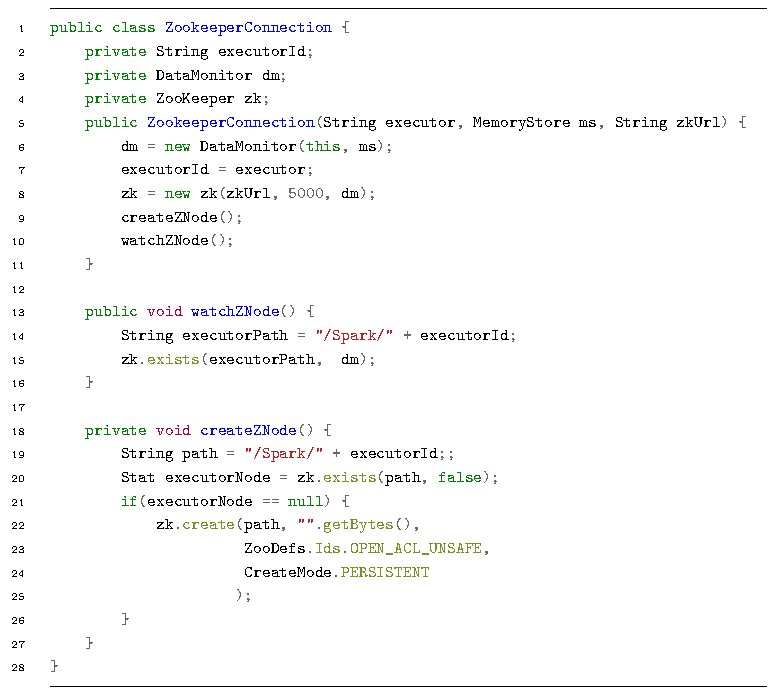
\includegraphics[scale=1.05]{imagens/conexao-zookeeper.pdf}
%     \end{center}
%     \small{Fonte: Próprio autor}
%     \label{fig:conexao-zookeeper}
% \end{figure}

% [corrigido]
\begin{figure}[!ht]
    \begin{algorithm}[H]
    \caption{Gerenciamento da Conexão com o ZooKeeper.}
        \label{fig:conexao-zookeeper}
            \KwData{\\
                dm $\leftarrow$ objeto o qual implementa o método \textit{process} do ZooKeeper para tratamento dos eventos\;
                Spark\_Executor\_id $\leftarrow$ identificador único do Executor do Spark\;
            }
    
            \SetKwProg{Fn}{Function}{}{end}
            \SetKwProg{Cs}{Class}{}{end}
            
            \Cs{ZookeeperConnection:} {
                zk $\leftarrow$ new ZooKeeper(Zk\_IP, timeout, dm)\; 
                
                \Fn{watchZnode()}{
                    myPath $\leftarrow$ getMyPath(Spark\_Executor\_id)\;
                    zk.exists(myPath, dm)\;
                }
                
                \BlankLine
                \Fn{createZnode()}{
                    myPath $\leftarrow$ getMyPath(Spark\_Executor\_id)\;
                    stat $\leftarrow$ zk.exists(myPath, dm)\;
                    
                    \If{$\nexists$ stat} {
                        zk.create(myPath, emptyData, ZooDefs.Ids.OPEN\_ACL\_UNSAFE, CreateMode. PERSISTENT)\;
                    }
                }
            }
    \end{algorithm}
\end{figure}


Conforme apresentado pelo Algoritmo \ref{fig:conexao-zookeeper}, a conexão do cliente junto ao ZooKeeper é gerenciada pela classe \textit{ZookeeperConnection}, implementada em Java. Esta classe recebe como parâmetros o identificador do \textit{Executor} onde está hospedada, a referência ao objeto \textit{MemoryStore} e a URL (\textit{Uniform Resource Location}) do nodo \textit{Master} do ZooKeeper. 

Durante a criação de um objeto desta classe, primeiro é realizada a inicialização do \textit{DataMonitor}, cujo objetivo é tratar os eventos gerados pelo ZooKeeper. A seguir, é salvo o identificador na classe e inicializada a conexão com o ZooKeeper (Linha 2), utilizando o endereço do nodo \textit{Master}, um \textit{timeout} e o objeto para tratamento dos eventos, isto é, o \textit{DataMonitor}.

Na sequência, cria-se o \textit{znode} responsável por representar o \textit{Executor} dentro da árvore \textit{in memory} do ZooKeeper, utilizando a função \textit{createZnode()} (Linhas 7--12). O caminho deste nodo é formado pelo prefixo \textit{/Spark/} seguido do seu identificador único, obtido através do \textit{BlockManager}. Uma representação visual desta estrutura é exibida na Figura \ref{fig:estrutura-utilizada-zookeeper}, apresentando a árvore de \textit{znodes} criada após a inicialização do \textit{cluster} Spark.

Por fim, registra-se o cliente do ZooKeeper utilizando a função \textit{watchZnode()}(Linhas 3--6), a fim de viabilizar o recebimento de notificações de eventos ocorridos na árvore de \textit{znodes}. Esse registro é efetuado apenas verificando a existência do nodo desejado. Após a ocorrência de um evento, o ZooKeeper irá informar todos os objetos registrados para realizar o tratamento da notificação.
 
\begin{figure}[!ht]
    \caption{Árvore de \textit{znodes} Criados pela Gerenciamento Dinâmico.}
    \begin{center}
        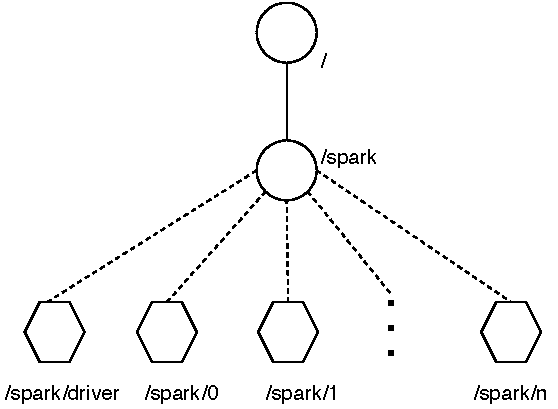
\includegraphics[scale=0.8]{imagens/estrutura-utilizada-zookeeper.pdf}
    \end{center}
    \small{Fonte: Próprio autor}
    \label{fig:estrutura-utilizada-zookeeper}
\end{figure}

Quando uma modificação ocorre em um \textit{znode}, todos os clientes são notificados pelo ZooKeeper, sendo repassado o caminho do nodo responsável pelo disparo do evento. Cabe a cada um dos clientes verificar se o nodo é de seu interesse e, caso seja necessário, realizar a remoção de dados da memória. A implementação do tratamento dos eventos recebidos pelo ZooKeeper é realizada através da função  demonstrada no Algoritmo \ref{fig:data-monitor-spark}. 

O Algoritmo \ref{fig:data-monitor-spark} implementa o método \textit{process}, de modo que este  seja sobrescrito a fim de implementar a lógica necessária para tratamento dos eventos disparados. Este método é exposto pela interface \textit{Watcher} provida pelo ZooKeeper. Desse modo, o ZooKeeper consegue notificar os clientes através de chamadas ao método \textit{process} de cada cliente conectado.

% \begin{figure}[!ht]
%     \caption{Tratamento de Eventos Recebidos.}
%     \begin{center}
%         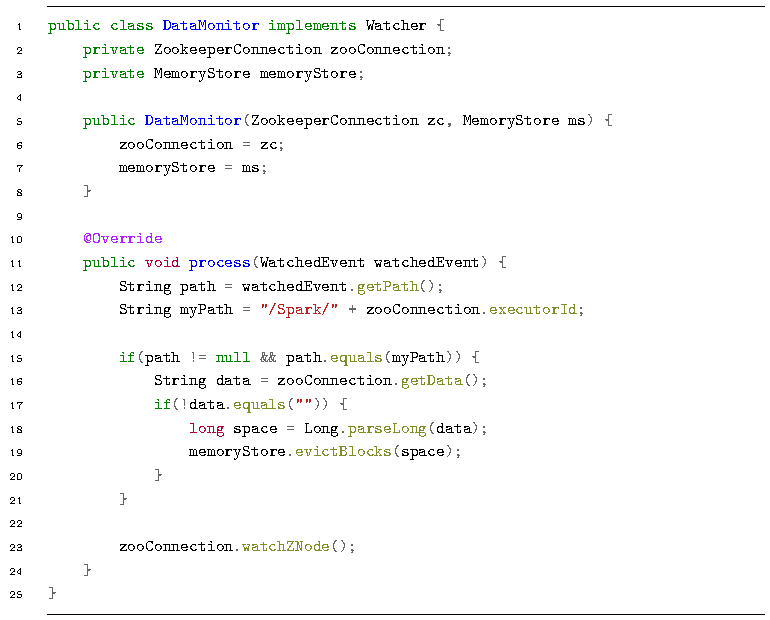
\includegraphics[scale=1]{imagens/data-monitor-spark.pdf}
%     \end{center}
%     \small{Fonte: Próprio autor}
%     \label{fig:data-monitor-spark}
% \end{figure}

\begin{figure}[!ht]
    \begin{algorithm}[H]
    \caption{Tratamento de Eventos Recebidos.}
        \label{fig:data-monitor-spark}
        \KwData{\\
            zooConnection $\leftarrow$ Conexão com o Zookeeper\;
            memoryStore $\leftarrow$ Objeto responsável pelo gerenciamento da memória do Spark\;
        }
        
        \BlankLine
        \emph{WatchedEvent é a classe de evento implementada pelo Zookeeper.}\\
        \SetKwProg{Fn}{Function}{}{end}
        \Fn{process(event: WatchedEvent)}{
            eventPath $\leftarrow$ event.getPath()\;
            myPath $\leftarrow$ getMyZonePath()\;
            
            \If{eventPath == myPath}{
                znodeData $\leftarrow$ zooConnection.getData()\;
                requiredBytes = Long(znodeData)\;
                memoryStore.evictBlocks(requiredBytes)\;
            }
            
            zooConnection.watchZnode()\;
        }
    \end{algorithm}
\end{figure}

Através do método \textit{process}, exibdo no Algoritmo \ref{fig:data-monitor-spark}, o \textit{Executor} recebe a notificação de uma mudança ocorrida nos dados associados às estruturas dos \textit{znodes}. A seguir, verifica-se em qual nodo ocorreu o evento (Linha 3). Caso o evento tenha ocorrido no \textit{znode} de interesse do \textit{Executor}, isto é, no nodo associado ao seu identificador único (Linhas 4 -- 5), deve-se remover blocos da memória. Essa remoção é realizada obtendo a quantidade de espaço que deve ser liberado, calculada e escrita pelo Agente de Monitoramento (Linhas 6--8). Ao final deve-se observar o znode de interesse, a fim de receber novas notificações relacionadas a alteração dos znodes mantidos pelo ZooKeeper (Linha 10).

\subsubsection{Agente de Monitoramento}
A última etapa para implementação do Gerenciamento Dinâmico refere-se ao desenvolvimento do Agente de Monitoramento, o qual permite a instrumentação da execução de aplicações Spark. Este agente tem como função determinar se dado o contexto da aplicação, isto é, \textit{status} de execução da aplicação e consumo de memória dos \textit{Executors}, deve-se ou não, remover partições da memória de forma antecipada.  

O Agente de Monitoramento consiste em uma aplicação desenvolvida na linguagem Java, com o objetivo de obter dados do Spark via API REST, de modo a prever a necessidade de liberação de espaço em memória no Spark durante a execução de aplicações. O agente é construído utilizando a API oficial do ZooKeeper para realizar a manipulação dos \textit{znodes} e, dessa forma, realizar a comunicação entre o Agente e os \textit{Executors} do Spark. 

A aplicação divide-se em três pacotes: \textit{Models}, \textit{Network} e \textit{Monitor}. A Figura \ref{fig:diagrama-pacotes} apresenta o Diagrama de Pacotes com as definições das classes as quais compõem cada pacote.

\begin{figure}[!ht]
    \caption{Diagrama de Pacotes do Agente de Monitoramento.}
    \begin{center}
        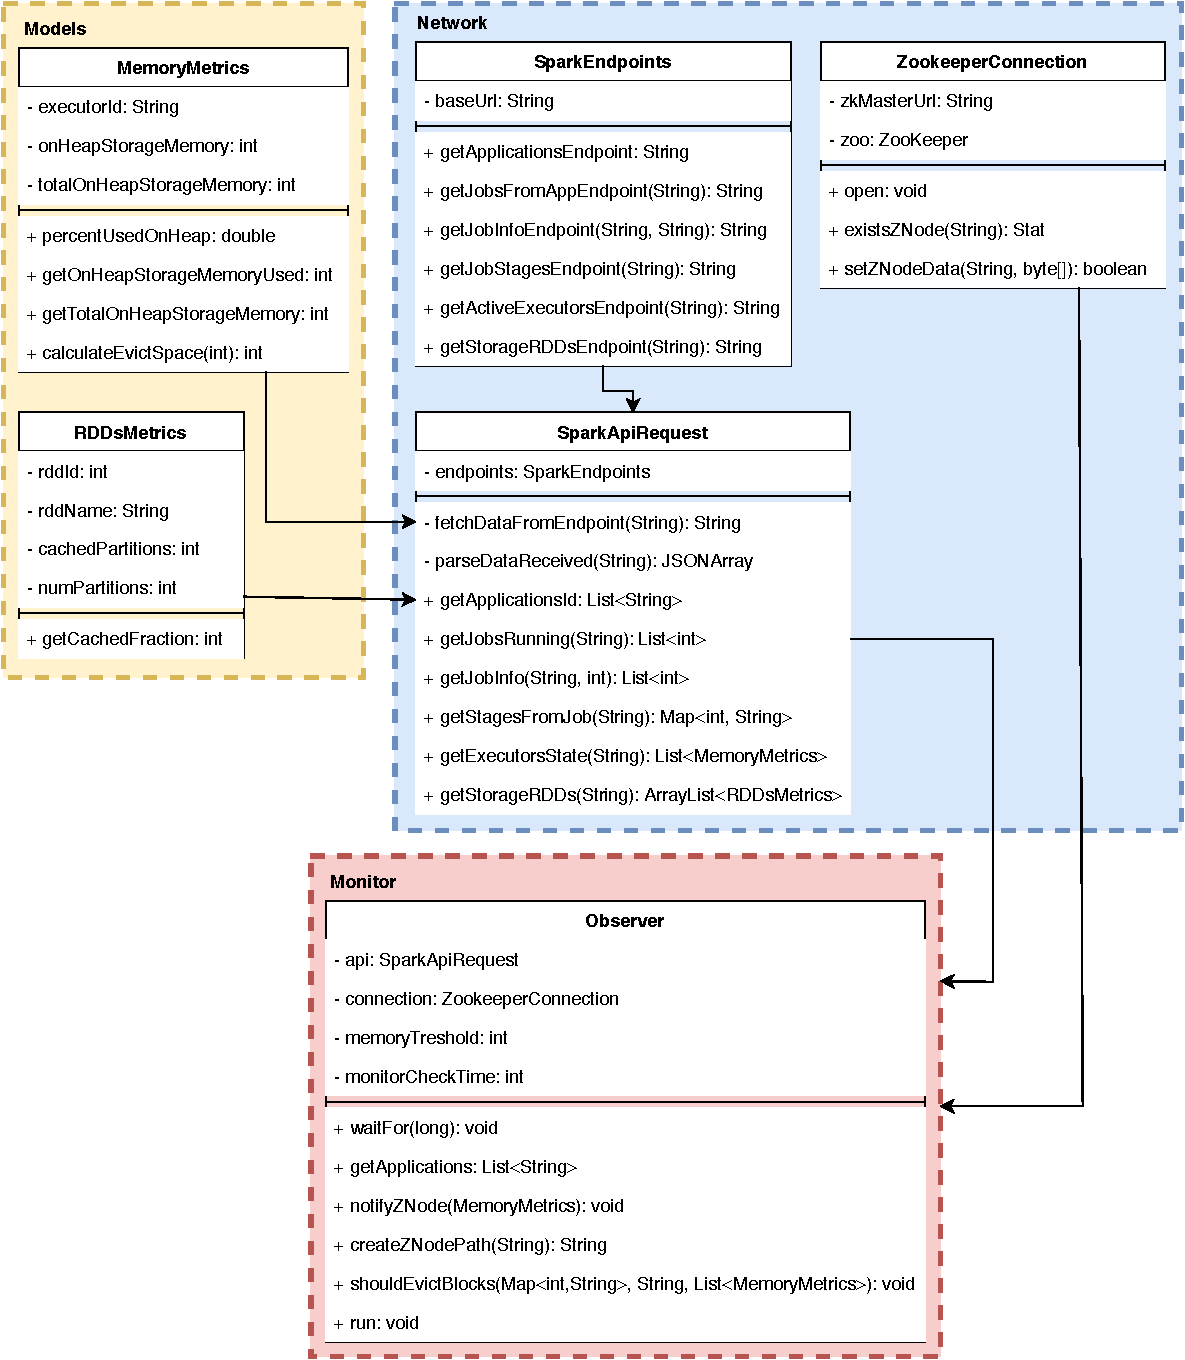
\includegraphics[scale=0.78]{imagens/diagrama-classe-v2.pdf}
    \end{center}
    \small{Fonte: Próprio autor}
    \label{fig:diagrama-pacotes}
\end{figure}

O pacote \textit{Models} oferece classes para encapsular as principais métricas obtidas através do Spark. Para tanto, agrupa-se os dados de interesse e são oferecidos métodos para melhorar a visualização dos dados coletados. Dessa forma, torna-se mais fácil a manipulação e o tratamento destas informações. Neste pacote encontram-se duas classes: \textit{MemoryMetrics} e \textit{RDDsMetrics}. 

A classe \textit{MemoryMetrics} armazena dados sobre o consumo de memória dos \textit{Executors} utilizados no processamento da aplicação. Assim, são armazenados o identificador do \textit{Executor}, o total de Memória de Armazenamento disponível e a quantidade de Memória de Armazenamento ocupada. Além disso, nesta classe são implementados os seguintes métodos:
\begin{enumerate}
    \item[a)] \textit{percentUsedOnHeap}: calcula a fração, em termos percentuais, do espaço consumido da Memória de Armazenamento;
    \item[b)] \textit{getOnHeapStorageMemoryUsed}: retorna o total, em \textit{bytes}, de Memória de Armazenamento utilizada pela aplicação;
    \item[c)] \textit{getTotalOnHeapStorageMemory}: retorna o total, em \textit{bytes}, de Memória de Armazenamento disponível para a aplicação;
    \item[d)] \textit{calculateEvictSpace(int)}: calula a quantidade de memória que deve ser removida do \textit{Executor}, baseando-se no \textit{threshold} passado por parâmetro para o método.
\end{enumerate}

Na classe \textit{RDDsMetrics} são armazenadas as informações relativas aos RDDs mantidos em \textit{cache}. Para tal, mantém-se o identificador do RDD, o número total de partições deste RDD e o número de partições armazenadas em memória. Além dos atributos responsáveis por armazenar as informações coletadas, esta classe implementa o método \textit{getCachedFraction}, responsável por calcular o percentual de partições mantidas em \textit{cache}.

O pacote \textit{Network} concentra as classes responsáveis pelo gerenciamento das conexões realizadas pela aplicação junto ao Spark e ao ZooKeeper. O gerenciamento destas conexões é feito através das classes \textit{SparkEndpoints}, \textit{SparkApiRequest} e \textit{ZookeeperConnection}.

Na classe \textit{SparkEnpoints}, encontram-se os métodos responsáveis por abstrair os \textit{Endpoints}, isto é, as URLs para acesso as informações do Spark. Para isto, esta classe formata as URLs corretamente com o identificador da aplicação e do \textit{job}, quando necessário, de modo a possibilitar que sejam utilizadas para realizar as requisições na API REST do Spark. 


A classe \textit{SparkApiRequest} tem como objetivo realizar as requisições através da API REST do Spark e obter informações sobre a aplicação, sendo estas requisições realizadas utilizando os \textit{endpoints} abstraídos pela classe \textit{SparkEndpoints}. Todo o tratamento dessas requisições é realizado por este componente, disponibilizando métodos para obter as informações necessárias para realizar o monitoramento da aplicação. Assim, os métodos disponibilizados por esta classe são:

\begin{enumerate}
    \item[a)] \textit{fetchDataFromEndpoint}: acessa o \textit{endpoint} recebido por parâmetro e retorna a resposta obtida. Retorna null em caso de falha;
    \item[b)] \textit{parseDataReceived}: decodifica o arquivo JSON recebido como resposta da requisição ao \textit{endpoint};
    \item[c)] \textit{getApplicationsId}: utiliza o \textit{endpoint /application} e retorna uma lista com todas as aplicações em execução;
    \item[d)] \textit{getJobsRunning}: acessa o \textit{endpoint /applications/{[}app-id{]}/jobs} e retorna os \textit{jobs} em execução da aplicação cujo identificador foi recebido como parâmetro;
    \item[e)] \textit{getJobInfo}: retorna os estágios que serão utilizados
    para processar o \textit{job}, obtidos através do \textit{endpoint /applications/{[}app-id{]}/jobs/{[}jib-id{]}};
    \item[f)] \textit{getStagesFromJob}: utiliza o \textit{endpoint /applications/{[}app-id{]}/stages} e retorna os estágios com seus respectivos status da aplicação informada no parâmetro;
    \item[g)] \textit{getExecutorsState}: Utiliza o \textit{endpoint /applications/{[}app-id{]}/executors} para coletar os dados relativos ao consumo de memória dos \textit{Executors} ativos na aplicação cujo identificador foi recebido por parâmetro;
    \item[h)] \textit{getStorageRDDs}: Através do \textit{endpoint /applications/{[}app-id{]}/storage/rdd}, obtém os RDDs mantidos em cache pela aplicação cujo identificador foi passado por parâmetro.
\end{enumerate}

A última classe contida no pacote \textit{Network} é a \textit{ZookeeperConnection}, a qual tem como objetivo gerenciar a conexão do Agente de Monitoramento com o nodo \textit{Master} do ZooKeeper. Os métodos oferecidos por essa classe visam abstrair a utilização da API do ZooKeeper de modo a facilitar a comunicação entre o agente e o ZooKeeper, possibilitando que seja realizada a notificação dos \textit{Executors}. Para isto, esta classe oferece os métodos:

\begin{enumerate}
    \item[a)] \textit{open}: cria uma nova conexão com o nodo \textit{Master} do ZooKeeper, permitindo acesso à árvore de \textit{znodes};
    \item[b)] \textit{existsZNode}: recebe como parâmetro uma string contendo o caminho do \textit{znode} o qual deseja verificar sua existência, retornando um objeto do ZooKeeper, do tipo \textit{Stat}, para indicar o \textit{status} do \textit{znode}.
    desse \textit{znode};
    \item[c)] \textit{setZNodeData}: recebe como parâmetro uma string com o caminho do \textit{znode} e um \textit{array} de \textit{bytes} com os dados que devem ser escritos no \textit{znode}. Retorna \textit{true} caso a operação tenha sido realizada com sucesso e \textit{false} em caso de falha ou inexistência do \textit{znode}.
\end{enumerate}

No pacote \textit{Monitor} encontra-se a classe \textit{Observer}, a qual contém a lógica principal para o monitoramento da aplicação. Para tanto, esta classe obtém as informações relacionadas à aplicação utilizando as classes implementadas nos pacotes \textit{Models} e \textit{Network}. A partir das informações, o Agente de Monitoramento decide se partições de RDDs devem ser removidas da memória. Para tanto, nesta classe são implementados os métodos:

\begin{enumerate}
    \item[a)] \textit{waitFor}: interrompe a execução da \textit{thread} por um determinado tempo, definido pelo parâmetro do método; 
    \item[b)] \textit{getApplications}: obtém as aplicações em execução. Esta função é executada até que seja encontrada, pelo menos, uma aplicação ativa no Spark;  
    \item[c)] \textit{notifyZNode}: calcula o espaço de memória que deve ser liberado e notifica o \textit{Executor} recebido por parâmetro;
    \item[d)] \textit{createZNodePath}: recebe uma string com o identificador do \textit{Executor} e retorna seu caminho na árvore de \textit{znodes};
    \item[e)] \textit{shouldEvictBlocks}: método responsável por determinar se partições de RDDs devem ser removidas da memória, baseando-se nas características do ambiente atual de execução;
    \item[f)] \textit{run}: função que executa a \textit{thread} principal de monitoramento do agente.
\end{enumerate}



A implementação do monitoramento é realizada em uma \textit{thread} separada, independente da \textit{thread} principal. Assim, é possível enviar comandos para o Agente de Monitoramento e, deste modo, acompanhar o percentual dos RDDs mantidos em \textit{cache}. Uma visão geral do fluxo de execução da \textit{thread} de  monitoramento é ilustrada pelo Algoritmo \ref{fig:thread-monitor}.

% \begin{figure}[!ht]
%     \caption{\textit{Thread} de Monitoramento da Aplicação.}
%     \begin{center}
%         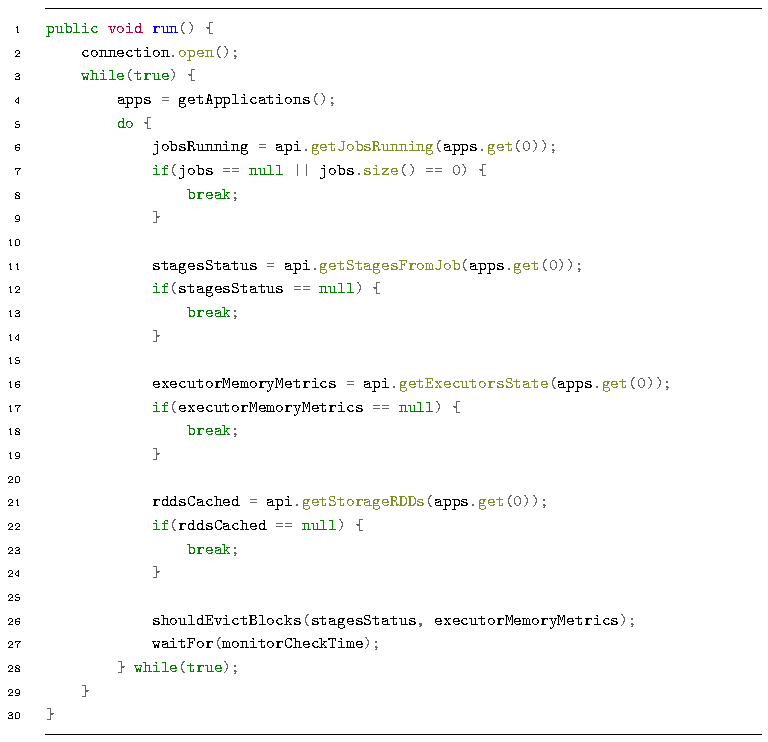
\includegraphics[scale=1]{imagens/thread-monitor-v2.pdf}
%     \end{center}
%     \small{Fonte: Próprio autor}
%     \label{fig:thread-monitor}
% \end{figure}

% [corrigido]
\begin{figure}[!ht] 
    \begin{algorithm}[H]
    \caption{\textit{Thread} de Monitoramento da Aplicação.}
        \label{fig:thread-monitor}
        \KwData{\\
            api $\leftarrow$ Conexão com o Zookeeper\;
            monitorCheckTime $\leftarrow$ Periodicidade do monitoramento\;
        }
        \SetKwProg{Fn}{Function}{}{end}
        \Fn{run()}{
            api $\leftarrow$ openZookeeperConnection()\;
            \While{True}{
                apps $\leftarrow$ getApplications()\;
                \While{True}{
                    jobsRunning $\leftarrow$ api.getJobsRunning()\;
                    stageStatus $\leftarrow$ api.getStageStatus(jobsRunning)\;
                    memoryMetrics $\leftarrow$ api.getMemoryMetrics(jobsRunning)\;
                    rddsCached $\leftarrow$ api.getRddsCached(jobsRunning)\;
                    
                    \BlankLine
                    \If{ocorreu erro na obtenção dos dados da api}{
                        break\;
                    }
                    
                    \BlankLine
                    shouldEvictBlocks(stageStatus, memoryMetrics)\;
                    waitFor(monitorCheckTime)\;
                }
            }
        }
    \end{algorithm}
\end{figure}

De acordo com o Algoritmo \ref{fig:thread-monitor}, para implementar a \textit{thread} de monitoramento, primeiro é inicializada a conexão entre o Agente de Monitoramento e o ZooKeeper (Linha 2). Um vez estabelecida a conexão, o monitoramento é realizado utilizando dois laços aninhados. O laço externo (Linhas 3--16) obtém as aplicações em execução no Spark através do método \textit{getApplications} (Linha 4). Este método é implementado para que seja possível obter os identificadores das aplicações em execução. Assim, garante-se a existência do identificador da aplicação para futuras requisições.

No laço interno (Linhas 5--15) são executadas as rotinas para coleta das métricas da aplicação implementadas pela classe \textit{SparkApiRequest} do pacote \textit{Network}. Primeiro, o agente obtém os \textit{jobs} da aplicação em execução (Linha 6). A seguir, coleta-se os estágios deste \textit{job} (Linha 7), juntamente com seus respectivos \textit{status}. Um estágio pode ter os seguintes \textit{status}: \textit{pending}, quando encontra-se pendente para execução; \textit{running} quando está em execução e \textit{completed} quando sua execução já foi realizada.

Na sequência, são reunidas as informações sobre os \textit{Executors} ativos na execução da aplicação (Linha 8). Nesta etapa, são extraídos os identificadores dos \textit{Executors} e as informações relativas ao consumo de memória. O identificador obtido nesta requisição é o mesmo utilizado para criar seu respectivo \textit{znode} no Zookeper. Desta forma, é possível notificar individualmente cada \textit{Executor}. A última requisição consiste na coleta das informações dos RDDs mantidos em \textit{cache} pela aplicação (Linha 9). A partir desta informação é possível determinar quais RDDs estão sendo mantidos em memória pela aplicação.

Após a execução de cada método utilizado para realizar o monitoramento (Linhas 6, 7, 8 e 9), deve-se verificar se o retorno dos método executado é igual a \textit{null}. Esta verificação é necessária para garantir que os dados foram corretamente obtidos (Linhas 10--12). Caso o retorno seja \textit{null}, a aplicação Spark finalizou sua execução durante o processamento do \textit{loop} interno (Linhas 5--15) e este deve ser finalizado através do comando \textit{break}. Na sequência, o laço externo (Linhas 3--16) volta a ser executado, obtendo novamente as aplicações em execução, já que o identificador da aplicação mudou pois trata-se de uma nova aplicação em execução.

Uma vez coletadas as métricas, o próximo passo consiste em verificar se há a necessidade de remover blocos da memória. Para isso, o método \textit{shouldEvictBlocks} (Linha 13) verifica os estágios do \textit{job}, bem como o consumo de memória dos \textit{Executors} da aplicação. Caso haja estágios pendentes para execução e o percentual de ocupação da memória esteja acima de um \textit{threshold} pré-estabelecido, uma notificação é enviada ao \textit{Executor} indicando que este deve remover partições de RDDs da memória. 
O \textit{threshold} é um limiar máximo para ocupação da memória utilizada pelo Spark, com valor inferior a 100\%. Por padrão, o Agente de Monitoramento adota um limiar de ocupação máximo de 95\%. Entretanto, o usuário pode configurar este valor no momento da inicialização do agente. 

Para realizar a notificação do \textit{Executor} cuja ocupação da memória excedeu o \textit{threshold} máximo, o Agente de Monitoramento calcula a quantidade de memória, em \textit{bytes}, acima do \textit{threshold} e escreve este valor no \textit{znode} correspondente ao \textit{Executor} modificando-o. Esta alteração é detectada pelo ZooKeeper, o qual envia uma notificação para todos os clientes conectados. O \textit{Executor} recebe esta informação contendo o espaço de memória que deve ser liberado e executa a remoção dos blocos de memória. A remoção de partições é realizada até que o espaço liberado pelo \textit{Executor} seja maior ou igual ao requisitado pelo Agente de Monitoramento.

% [corrigido: nao, porque não fiz a coleta de dados em diferentes tempos para a periodicidade do monitoramento. Nos experimentos, constatei que com 2s em diante, o spark removia dados por conta e depois chegava uma notificacao (atrasada) do monitoramento] | Comentario: Fez essa análise? Poderia colocar? Qual é o impacto real de sobrecarga para diferentes intervalos? 
Uma iteração do laço interno (Linhas 5--15) é finalizada aguardando um tempo pré-estabelecido, até que a próxima iteração deste mesmo laço execute e toda a computação seja realizada novamente. Por padrão, realiza-se uma iteração por segundo, de modo a acompanhar constantemente a evolução da ocupação da memória. Intervalos de tempo superiores tendem a deixar a memória sobrecarregada, induzindo o Spark a gerenciar a memória de forma reativa. Assim como o \textit{threshold}, a periodicidade com que o laço será executado pode alterada pelo usuário através dos parâmetros de entrada da aplicação, via linha de comando.


\subsection{Experimentos e Resultados}
O processo de validação do modelo de Gerenciamento Dinâmico implementado foi realizado na plataforma Grid'5000, utilizando um \textit{cluster} com 8 nodos. Assim como os experimentos realizados utilizando o Algoritmo Baseando em Prioridades, a experimentação do modelo de Gerenciamento Dinâmico foi feita utilizando 7 nodos para o Spark, gerando diferentes cargas de acesso a memória. Entretanto, adicionou-se um 8º nodo ao \textit{clustes} a fim de hospedar o Agente de Monitoramento e o ZooKeeper. A adição deste nodo visa evitar que haja uma sobrecarga nos nodos utilizados pelo Spark, isolando as computações requeridas por estas aplicações em um nodo dedicado.

Assim, os 8 nodos selecionados foram configurados da seguinte maneira: 1 Spark \textit{Master}, 4 Spark \textit{Workers}, 1 nodo executando o \textit{HDFS Namenode} e \textit{HDFS Datanode}, 1 nodo executando o \textit{HDFS Datanode} e 1 nodo hospedando o Agente de Monitoramento e o ZooKeeper \textit{Master}. Cada nodo do sistema era composto por dois  Intel Xeon E5-2630 v3 @2.4GHz (8 \textit{cores}/CPU), 128GB de memória RAM e dois HDs 600GB, conectados via quatro \textit{ethernet} 10Gbps. O sistema operacional utilizado foi o Debian 8, juntamente com Java JDK 1.8.202, Spark 2.2.0 e Hadoop 2.7.1.

Os experimentos foram realizados utilizando os algoritmos \textit{PageRank}, \textit{K-Means} e \textit{Logistic Regression} como \textit{benchmarks}, com o \textit{dateset large} como conjunto de dados de entrada. Tanto os \textit{benchmarks} quanto o \textit{dataset} utilizados na validação do modelo de gerenciamento foram implementados pelo Intel HiBench \cite{huang2010hibench}. Através destes \textit{benchmarks}, visava-se criar 3 possíveis cenários com reutilização de dados:

\begin{enumerate}
    \item[a)] \textit{PageRank}: acesso intensivo à memória, mas sem substituição de dados do \textit{benchmark};
    \item[b)] \textit{K-Means}: adição e remoção de RDDs mantidos em \textit{cache} durante a execução do \textit{benchmark}, além da remoção de dados da memória e; 
    \item[c)] \textit{Logistic Regression}: ocorrência de remoção de dados durante o processamento do \textit{benchmark}, mas sem realizar a remoção de RDDs da \textit{cache} ao longo de toda execução.
\end{enumerate}

Ainda, para cada \textit{benchmark} foram criados cinco configurações de memória total disponível: 1 GB, 1,5 GB, 2 GB, 2,5 GB e 3 GB. Diferentemente dos experimentos realizados na Seção \ref{sec:alg-pesos}, na validação do modelo de gerenciamento optou-se por remover a configuração de 4 GB disponíveis, uma vez que este não causa sobrecarga à memória, tornando indiferente o algoritmo de gerenciamento de memória utilizado. 

Por fim, foram incluídas as configurações de 2,5 GB e 3 GB de memória disponível. A inclusão destas configurações teve como objetivo criar cenários com intervalos regulares de 0,5 GB a fim de verificar o comportamento da execução dos \textit{benchmarks} utilizados. Na Tabela \ref{tab:memoria-arq-dinamica}, são demonstrados os valores de Memória Total, Memória de Armazenamento e Memória de Armazenamento Total obtidos a partir das cinco configurações utilizadas.

\begin{table}[!ht]
    \caption{Configuração de Memória Utilizada - Gerenciamento Dinâmico}
    \label{tab:memoria-arq-dinamica}
    \centering
    \scalebox{0.9}{
    \begin{tabular}{ccc}
        \hline
        Memória Total & Memória de Armazenamento & Memória Total de Armazenamento Disponível \\ \hline
        1 GB & 366,3 MB & 1465,2 MB \\
        1,5 GB & 639,3 MB & 2557,2 MB \\
        2 GB & 912,3 MB & 3649,2 MB \\
        2,5 GB & 1185,6 MB & 4742,4 MB \\
        3 GB & 1458,6 MB & 5834,4 MB \\ \hline
    \end{tabular}
}
\end{table}

Para a realização dos experimentos, as únicas configurações exigidas pelo ZooKeeper consistem na porta utilizada pelos clientes para realizar a conexão -- sendo 2181 a porta padrão --, um diretório para armazenamento de \textit{snapshots} do estado da memória e um \textit{tick time}, responsável por definir a periodicidade de mensagens \textit{heartbeat} enviadas pelo \textit{framework} a fim de verificar se a conexão dos clientes ainda encontra-se ativa.

O Agente de Monitoramento foi configurado para realizar a verificação do consumo de memória dos \textit{Executors} de forma constante, sendo esta realizada uma vez por segundo. Esta janela de tempo foi escolhida visto que as \textit{tasks} podem ser rapidamente executadas e o espaço disponível na memória ser completamente ocupado.

O \textit{threshold} de ocupação da memória foi adotado em 95\%, visando deixar 5\% da Memória de Armazenamento livre em situações onde é identificada a necessidade de novas computações. A escolha desse \textit{threshold} foi feita de maneira experimental, isto é, após testes preliminares utilizando quatro configurações de \textit{thresholds}: 80\%, 85\%, 90\% e 95\%. A partir destes experimentos preliminares, foi possível perceber que o limiar de ocupação de 95\% apresentou o melhor desempenho.

Na prática, utilizar um \textit{threshold} baixo implica em limitar o espaço disponível para armazenamento de informações. Por exemplo, em uma configuração onde há 2,5 GB de memória total e utiliza-se um \textit{threshold} de 70\%, o espaço disponível para armazenamento de informações é equivalente a 638,61 MB, sendo este valor equivalente a configuração de 2 GB onde há 639,3MB disponíveis.


Deste modo, os valores utilizados para as métricas de Frequência de Monitoramento e \textit{threshold} foram escolhidos após a realização de experimentos com configurações distintas. Estes experimentos visavam variar a frequência do monitoramento, isto é, o tempo entre cada verificação do consumo de memória, e o \textit{threshold} utilizados. Assim, os valores dos parâmetros adotados na experimentação final foram aqueles que apresentaram resultados mais promissores dentre as configurações avaliadas. Por fim, os resultados apresentados são obtidos a partir da média aritmética de 20 execuções para cada configuração. 

\subsubsection{Pagerank}
O \textit{PageRank} é um \textit{benchmark} cujo objetivo é classificar \textit{links} baseando-se em suas ligações, visando determinar uma relevância para cada \textit{link}, onde a precisão dessa classificação depende do número de iterações. Este \textit{benchmark} tinha como objetivo gerar um cenário com acesso intensivo à memória, mas sem substituição de dados do \textit{benchmark}.

No Spark, o processamento deste \textit{benchmark} é realizado em apenas um único \textit{job}. Ou seja, os RDDs responsáveis por calcular a relevância de cada \textit{link} são criados e, ao final, utiliza-se uma ação para submeter a \textit{lineage} ao \textit{DAGScheduler} e iniciar o processamento do \textit{benchmark}.

A \textit{lineage} gerada pelo \textit{benchmark} é composta por 30 RDDs, onde há reutilização do RDD com identificador 6 em outros 4 novos RDDs. Estes RDDs utilizados pelo \textit{benchmark} são processados pelo Spark em 6 estágios de execução. Assim, os resultados obtidos são demonstrados pela Tabela \ref{tab:resultados-pagerank-arq-dinamica} e pela Figura \ref{fig:arq-dinamica-pagerank}, sendo estes resultados a média aritmética de 20 execuções.


\begin{table}[!ht]
    \caption{Tempos de Execuções Obtidos no \textit{Benchmark} \textit{PageRank}}
    \label{tab:resultados-pagerank-arq-dinamica}
    \centering
    \scalebox{1}{
    \begin{tabular}{ccccc}
        \hline
         Algoritmo & \begin{tabular}[c]{@{}c@{}}Memória \\ Disponível\end{tabular} & \begin{tabular}[c]{@{}c@{}}Tempo de \\ Execução (em s)\end{tabular} & \begin{tabular}[c]{@{}c@{}}Desvio \\ Padrão (em s)\end{tabular} \\ \hline
        LRU & \multirow{2}{*}{1 GB} & 292,28 & 27,41 \\
        Gerenc. Dinâmico &  & 192,46 & 40,12 \\ \hline
        LRU & \multirow{2}{*}{1,5 GB} & 77,92 & 5,33 \\
        Gerenc. Dinâmico &  & 78,68 & 1,99 \\ \hline
        LRU & \multirow{2}{*}{2 GB} & 47,87 & 0,93 \\
        Gerenc. Dinâmico &  & 48,81 & 1,01 \\ \hline
        LRU & \multirow{2}{*}{2,5 GB} & 44,56 & 0,64 \\
        Gerenc. Dinâmico &  & 45,05 & 0,57 \\ \hline
        LRU & \multirow{2}{*}{3 GB} & 45,23 & 2,94 \\
        Gerenc. Dinâmico &  & 44,92 & 0,97 \\ \hline
    \end{tabular}
    }
\end{table}

\begin{figure}[!ht]
    \caption{Tempos de Execução do \textit{benchmark PageRank}}
    \begin{center}
        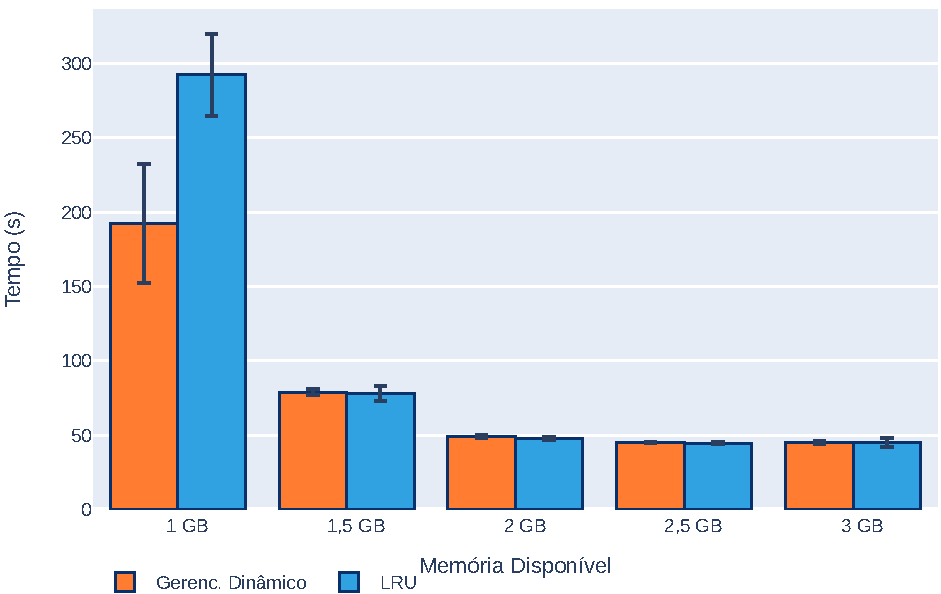
\includegraphics[scale=0.95]{imagens/Gerenc-PageRank.pdf}
    \end{center}
    \small{Fonte: Próprio autor}
    \label{fig:arq-dinamica-pagerank}
\end{figure}

A diferença mais notável foi detectada na configuração com 1 GB de memória disponível. Nesta configuração, o Gerenciamento Dinâmico foi, em média, 34,15\% mais rápido que o algoritmo LRU nas mesmas condições. Analisando os \textit{logs} de execução produzidos durante a execução deste \textit{benchmark}, é possível perceber que não houve remoção de partições de RDDs da memória em ambos os casos, tanto com a utilização do algoritmo LRU quanto o Gerenciamento Dinâmico. Isto se dá mesmo em casos de restrição de memória total, como é possível perceber no uso de 1 GB. 

Na execução deste \textit{benchmark}, apenas variáveis de \textit{broadcasts}, as quais são utilizadas para sincronizar a execução entre os nodos do \textit{cluster}, são removidas da memória. Neste processo, é possível perceber que o LRU introduz de forma mais frequente um \textit{overhead} na remoção, pela JVM, dos objetos não mais utilizados, sendo este fato demonstrado pelo exceção \textit{GC Overhead Limit Exceeded error}. 

A sobrecarga na remoção de objetos pela JVM é causada pela forma  de implementação do LRU no Spark. O Spark utiliza-se de uma lista dinâmica, inicialmente com 32 posições, sendo novas posições alocadas quando a lista atinge 75\% de ocupação. Assim, a remoção de blocos na memória de execução e na memória de dados sobrecarrega o \textit{Garbage Collector}. 

Diferentemente do LRU, a implementação do modelo de Gerenciamento Dinâmico utiliza uma estrutura onde não há alocação de memória realizada de maneira prévia. Desde modo, aloca-se espaço na memória apenas quando há 
necessidade de armazenar novos dados. Como consequência, o Gerenciamento Dinâmico consegue atingir uma mais estabilidade na execução deste \textit{benchmark} em situações onde há uma alta sobrecarga no acesso a memória e o espaço disponível total é reduzido, acarretando em uma diminuição do tempo médio de execução.

\subsubsection{K-Means}
O \textit{benchmark K-Means} é uma aplicação de aprendizagem de máquina de forma não supervisionada, cujo objetivo é agrupar o conjunto de dados utilizados como entrada em \textit{K} grupos distintos. Este agrupamento é realizado utilizando as características encontradas no conjunto de dados. Uma particularidade deste \textit{benchmark} é a manipulação dos RRDs mantidos em \textit{cache}, onde diferentes RDDs são reutilizados na criação de novos RDDs.

No \textit{benchmark} \textit{K-Means} é esperado que RDDs sejam adicionados e removidos da \textit{cache}. A \textit{lineage} formada pela implementação desse \textit{benchmark} é composta por 31 RDDs, dos quais 4 são mantidos em \textit{cache}, sendo estes os RDDs 2, 3, 9 e 13. Os RDDs 9 e 13 são adicionados e posteriormente removidos da \textit{cache} no decorrer da execução da aplicação. Os RDDs 2 e 3 apresentam as maiores frequências de reutilização, sendo mantidos em \textit{cache} durante toda a execução do \textit{benchmark}.

Os resultados, obtidos a partir da média aritmética de 20 execuções, deste \textit{benchmark} são demonstrados na Tabela \ref{tab:resultados-kmeans-arq-dinamica} e na Figura \ref{fig:arq-dinamica-kmeans}. 

\begin{table}[!ht]
    \caption{Tempos de Execuções Obtidos no \textit{Benchmark} \textit{K-Means}}
    \label{tab:resultados-kmeans-arq-dinamica}
    \centering
    \scalebox{1}{
    \begin{tabular}{ccccc}
        \hline
        Algoritmo & \begin{tabular}[c]{@{}c@{}}Memória \\ Disponível\end{tabular} & \begin{tabular}[c]{@{}c@{}}Tempo de \\ Execução (em s)\end{tabular} & \begin{tabular}[c]{@{}c@{}}Desvio \\ Padrão (em s)\end{tabular} \\ \hline
        LRU & \multirow{2}{*}{1 GB} & 155,79 & 6,60 \\
        Gerenc. Dinâmico &  & 148,84 & 6,75 \\ \hline
        LRU & \multirow{2}{*}{1,5 GB} & 167,36 & 3,08 \\
        Gerenc. Dinâmico &  & 166,07 & 4,25 \\ \hline
        LRU & \multirow{2}{*}{2 GB} & 116,47 & 4,95 \\
        Gerenc. Dinâmico &  & 108,28 & 2,41 \\ \hline
        LRU & \multirow{2}{*}{2,5 GB} & 43,93 & 3,31 \\
        Gerenc. Dinâmico &  & 44,19 & 1,89 \\ \hline
        LRU & \multirow{2}{*}{3 GB} & 46,26 & 3,55 \\
        Gerenc. Dinâmico &  & 46,72 & 4,21 \\ \hline
    \end{tabular}
    }
\end{table}

\begin{figure}[!ht]
    \caption{Tempos de Execução do \textit{benchmark K-Means}.}
    \begin{center}
        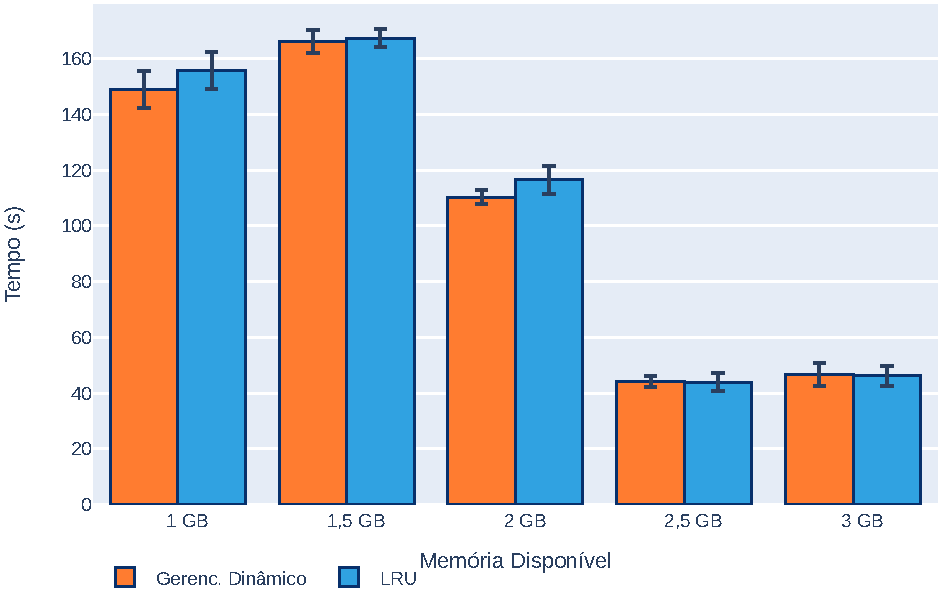
\includegraphics[scale=1.0]{imagens/Gerenc-K-Means.pdf}
    \end{center}
    \small{Fonte: Próprio autor}
    \label{fig:arq-dinamica-kmeans}
\end{figure}

Analisando os resultados obtidos neste \textit{benchmark}, as diferenças mais perceptíveis foram detectadas nas configurações de 1 GB e 2 GB de memória total disponível. Com 1 GB, o modelo de Gerenciamento Dinâmico foi aproximadamente 4,46\% mais rápido, quando comparado ao LRU. Já na configuração de 2 GB de memória, o modelo de gerenciamento foi 7,89\% mais rápido que o LRU nas mesmas condições, quando consideramos a média dos tempos de execução destes \textit{benchmarks}. 

Nas configurações de 1,5 GB, 2,5 GB e 3 GB de memória disponível, o desempenho de ambos algoritmos foi equivalente. Analisando os \textit{logs} de execução gerados pelo \textit{K-Means}, observou-se que a execução deste \textit{benchmark} se deu em 14 \textit{jobs}, sendo 7 \textit{jobs} compostos por um estágio e os demais compostos por 2 ou 3 estágios. Em casos onde o \textit{job} é composto por apenas um  estágio, não há possibilidade de prever a existência de computações futuras. Esta restrição ocorre uma vez que o Spark executa as aplicações gerando o plano de execução do \textit{jobs} apenas quando ações são aplicadas ao RDD.

Assim, nos \textit{jobs} com um estágio é inviável analisar a aplicação de forma integral a fim de verificar se outros \textit{jobs} serão necessários para completar execução. Consequentemente, o Agente de Monitoramento opta por não remover dados da memória, mesmo em situações onde o \textit{threshold} foi ultrapassado.

Uma diferença evidente entre o algoritmo LRU e o modelo de Gerenciamento Dinâmico é a forma como os blocos de dados são operados. Na Tabela \ref{tab:resultados-substitucoes-kmeans} é exibido o número de inserções e remoções realizadas na memória em cada configuração testada. A partir desta tabela, busca-se investigar e apresentar o comportamento das operações ocorridas em memória, quando utilizado o LRU e o algoritmo de Gerenciamento Dinâmico.

A tabela descreve o número de partições de RDDs adicionadas e removidas da memória e a quantidade de variáveis de \textit{broadcast} adicionadas e removidas. As partições são blocos que contém os dados em \textit{cache} da aplicação, enquanto as variáveis de \textit{broadcast} são utilizadas pelo Spark para distribuir as \textit{tasks} entre os \textit{Executors}. Os valores apresentados são a média aritmética das 20 execuções realizadas em cada configuração de memória.

\begin{table}[!ht]
\caption{Número de Remoções e Inserções de Dados na Memória do \textit{benchmark} K-Means}
    \label{tab:resultados-substitucoes-kmeans}
    \centering
    \begin{tabular}{cccccc}
    \hline
        Algoritmo & Memória & \begin{tabular}[c]{@{}c@{}}Partições \\ de RDDs \\ Adicionadas\end{tabular} & \begin{tabular}[c]{@{}c@{}}Partições \\ de RDDs\\  Removidas\end{tabular} & \begin{tabular}[c]{@{}c@{}}Variáveis \\ de Broadcast \\ Adicionadas\end{tabular} & \begin{tabular}[c]{@{}c@{}}Variáveis \\ de Broadcast \\ Removidas\end{tabular} \\ \hline
        LRU & \multirow{2}{*}{1 GB} & 185 & 108 & 147 & 119 \\
        Gerenc. Dinâmico &  & 188 & 109 & 147 & 115 \\ \hline
        LRU & \multirow{2}{*}{1,5 GB} & 356 & 265 & 146 & 63 \\
        Gerenc. Dinâmico &  & 362 & 270 & 146 & 115 \\ \hline
        LRU & \multirow{2}{*}{2 GB} & 247 & 150 & 146 & 65 \\
        Gerenc. Dinâmico &  & 210 & 116 & 146 & 111 \\ \hline
        LRU & \multirow{2}{*}{2,5 GB} & 132 & 12 & 146 & 63 \\
        Gerenc. Dinâmico &  & 134 & 14 & 146 & 60 \\ \hline
        LRU & \multirow{2}{*}{3 GB} & 133 & 14 & 146 & 57 \\
        Gerenc. Dinâmico &  & 145 & 25 & 146 & 60 \\ \hline
    \end{tabular}
\end{table}

De acordo com a Tabela \ref{tab:resultados-substitucoes-kmeans}, com 1 GB de memória, tanto o LRU quanto o Gerenciamento Dinâmico removeram e inseriram uma quantidade semelhante de partições de RDDs e variáveis de \textit{broadcast} durante a execução do \textit{benchmark}. Esta semelhança na quantidade de remoções e inserções de dados na memória demonstra que, nessas condições, a memória encontrava-se fortemente sobrecarregada. Nas configurações de 1,5 GB, a diferença principal foi na quantidade de variáveis de \textit{broadcast} removidas pelo modelo de gerenciamento. Nesta configuração, o Gerenciamento Dinâmico removeu mais variáveis de \textit{broadcast}, e consequentemente manteve mais partições de RDDs em memória. 

Na configuração de 2 GB de memória é observada a maior diferença entre os métodos de gerenciamento de memória. Nesta configuração, o Gerenciamento Dinâmico removeu uma quantidade menor de partições de RDDs da memória, havendo também uma redução no número de inserções de partições. Estas reduções ocorrem porque o algoritmo utilizado para gerenciar a memória no modelo de Gerenciamento Dinâmico consegue priorizar partições de RDDs em detrimento das variáveis de \textit{broadcast}. Assim, enquanto o LRU remove uma partição de RDD para inserir outra partição de RDD, o algoritmo utilizado o Gerenciamento Dinâmico remove primeiro as variáveis de \textit{broadcast}, para então remover dados.

Quando utilizadas as configurações de 2,5 GB e 3G GB de memória, o comportamento de ambos algoritmos foi similar, ou seja, tanto o tempo de execução quanto o número de operações de adição e remoção de blocos da memória foram semelhantes. Esta semelhança se dá devido ao o espaço disponibilizado se mostrou próximo do suficiente para comportar todo o \textit{dataset}, exigindo poucas operações de adição e remoção de dados da memória.

Portanto, ao sumarizar as informações das Tabelas  \ref{tab:resultados-kmeans-arq-dinamica} e  \ref{tab:resultados-substitucoes-kmeans}, o algoritmo utilizado no Gerenciamento Dinâmico tende a priorizar a manutenção de partições de RDDs em detrimento das variáveis de \textit{broadcast}. Deste modo, esta característica na ordem de remoção dos dados difere entre o LRU e o algoritmo utilizado no Gerenciamento Dinâmico. Assim, em situações onde há restrição no espaço de memória disponível, como o ocorrido nos casos com 1,5 GB e 2 GB de memória total, onde o Gerenciamento Dinâmico removeu uma maior quantidade de variáveis de \textit{broadcast}. Além disto, o Gerenciamento dinâmico conseguiu reduzir o tempo de execução necessário nas configurações de 1 GB, 1,5 GB e 2 GB.


\subsubsection{Logistic Regression}
O \textit{benchmark Logistic Regression} consiste em um tipo de análise estatística utilizada frequentemente para análise preditiva. Diferente dos \textit{benchmarks} anteriores, a principal característica do \textit{Logistic Regression} está na permanência de RDDs em memória. Assim, dois RDDs são computados e mantidos em \textit{cache} durante toda a execução deste \textit{benchmark}. Dessa forma, não há remoção de RDDs da \textit{cache} como ocorrido no \textit{K-Means}.

Durante a computação desse \textit{benchmark}, ao total são manipulados 157 RDDs, sendo os RDDs 2 e 11 mantidos em \textit{cache} pernamentemente durante a execução do \textit{benchmark}. Estes RDDs manipulados são processados em 42 \textit{jobs}, dentre os quais apenas 2 são compostos por um único estágio. Assim, torna-se possível identificar se novas computações serão requeridas pelo \textit{job} e, se necessário, realizar a remoção antecipada de blocos da memória.

Além disso, o \textit{benchmark Logistic Regression} possui o maior \textit{dataset} dentre os \textit{benchmarks} utilizados, com um total de 7,5 GB de dados. Assim, devido ao grande número de RDDs processados e ao conjunto de dados utilizado, este \textit{benchmark} utiliza a memória de maneira mais intensiva.

Os resultados obtidos, sendo estes a média aritmética de 20 execução em cada configuração, são demonstrados na Tabela \ref{tab:resultados-lr-arq-dinamica} e na Figura \ref{fig:arq-dinamica-lr}. A Tabela \ref{tab:resultados-substitucoes-lr} demonstra a quantidade média de operações de adição e remoção de blocos da memória durante a execução.

\begin{table}[!ht]
    \caption{Tempos de Execuções Obtidos no \textit{Benchmark} \textit{Logistic Regression}}
    \label{tab:resultados-lr-arq-dinamica}
    \centering
    \scalebox{1}{
    \begin{tabular}{ccccc}
        \hline
        Algoritmo & \begin{tabular}[c]{@{}c@{}}Memória \\ Disponível\end{tabular} & \begin{tabular}[c]{@{}c@{}}Tempo de \\ Execução (em s)\end{tabular} & \begin{tabular}[c]{@{}c@{}}Desvio \\ Padrão (em s)\end{tabular} \\ \hline
        LRU & \multirow{2}{*}{1 GB} & 0 & 0 \\
        Gerenc. Dinâmico &  & 0 & 0 \\ \hline
        LRU & \multirow{2}{*}{1,5 GB} & 469,67* & 0,0* \\
        Gerenc. Dinâmico &  & 357,22 & 12,69 \\ \hline
        LRU & \multirow{2}{*}{2 GB} & 305,94 & 4,80 \\
        Gerenc. Dinâmico &  & 289,76 & 2,30 \\ \hline
        LRU & \multirow{2}{*}{2,5 GB} & 255,91 & 7,34 \\
        Gerenc. Dinâmico &  & 245,84 & 2,44 \\ \hline
        LRU & \multirow{2}{*}{3 GB} & 140,60 & 10,70 \\
        Gerenc. Dinâmico &  & 150,11 & 15,85 \\ \hline
    \end{tabular}
    }
\end{table}

\begin{figure}[!ht]
    \caption{Tempos de Execução do \textit{benchmark Logistic Regression}.}
    \begin{center}
        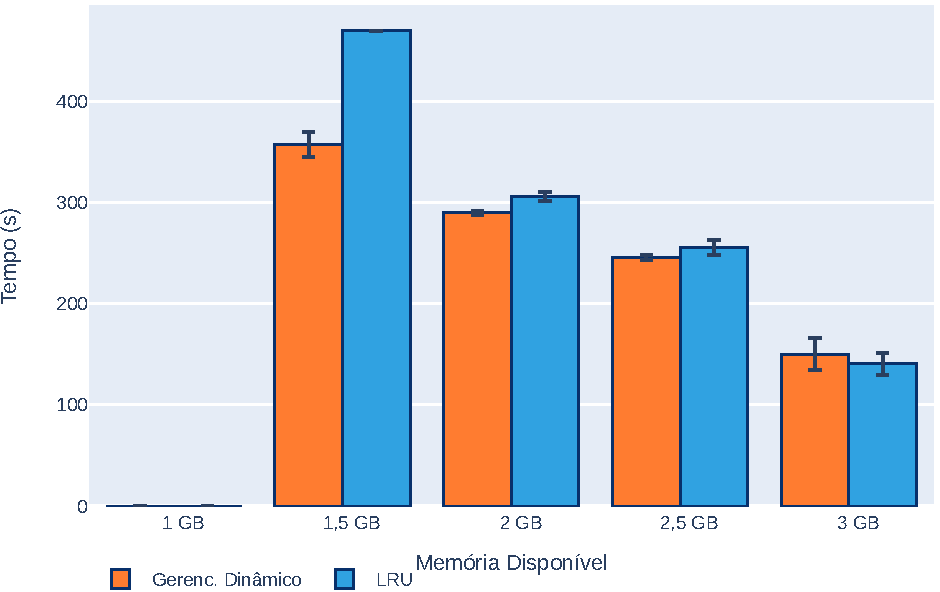
\includegraphics[scale=1.0]{imagens/Gerenc-Logistic-Regression.pdf}
    \end{center}
    \small{Fonte: Próprio autor}
    \label{fig:arq-dinamica-lr}
\end{figure}

Analisando a Tabela \ref{tab:resultados-lr-arq-dinamica}, na configuração com 1 GB de memória total disponível, tanto o algoritmo LRU quanto o modelo de Gerenciamento Dinâmico não conseguiram terminar a execução da aplicação. Nestes casos, uma exceção de \textit{OutOfMemoryError} é lançada pela JVM, indicando uma alta sobrecarga no tempo de execução do \textit{Garbage Collector} (GC) e interrompendo a execução do \textit{benchmark}, sendo este comportamento observado durante as 20 execuções do \textit{benchmark}, em ambos os algoritmos. É importante ressaltar que todas as execuções foram realizadas utilizando o algoritmo padrão de GC provido pela Oracle Java JDK 1.8.

Observando os resultados atingidos, nota-se uma singularidade com relação a configuração com capacidade de 1,5 GB de memória total disponível.Nesta configuração, o algoritmo LRU não conseguiu completar nenhuma execução deste \textit{benchmark}. O tempo demonstrado pela Tabela \ref{tab:resultados-lr-arq-dinamica} para a configuração de 1,5 GB do LRU é aquele capturado pelo HiBench para execução de 29 dos 42 \textit{jobs} da aplicação. Assim, o modelo de Gerenciamento Dinâmico foi, em média, 23,94\% mais rápido que o tempo registrado para o LRU, mesmo que este algoritmo não tenha terminado o processamento da aplicação por completo. 

Além disso, houve uma grande discrepância na estabilidade do Spark durante a execução do \textit{benchmark} nesta configuração de 1,5 GB, onde o algoritmo LRU conseguiu executar apenas 1 vez dentre todas as tentativas realizadas, impossibilitando o cálculo do desvio padrão do tempo médio de execução. Assim como o ocorrido na configuração com 1 GB disponível, as 19 execuções restantes foram interrompidas pela JVM indicando sobrecarga nas rotinas do \textit{Garbage Collector}.

Quando dispostos 2 GB de memória total disponível, o Gerenciamento Dinâmico foi 11,82\% mais rápido, quando comparado ao LRU nesta mesma configuração e considerado a média das execuções. Em situações com 2,5 GB, ambos os métodos de gerenciamento de memória apresentaram desempenho similar, havendo uma redução de apenas 3,93\% no tempo de execução do LRU. Na última configuração avaliada, com 3 GB de memória disponível, o modelo de gerenciamento implementado foi 6,37\% mais lento que o LRU, acarretando em uma degradação no desempenho. Esta degradação ocorreu devido ao \textit{threshold} adotado, induzindo o aumento na remoção de blocos da memória a fim de evitar o preenchimento completo da memória.

A Tabela \ref{tab:resultados-substitucoes-lr} tem como objetivo demonstrar o número de inserções e remoções de dados na memória, durante a execução do \textit{benchmark}. Na configuração de 1 GB de memória disponível, nenhuma informação relativa às operações na memória foi capturada, visto que ambos algoritmos não conseguiram finalizar a execução do \textit{benchmark}.

Quando utilizada a configuração com 1,5 GB de memória disponível, não foi possível obter os dados relativos ao comportamento da memória do algoritmo LRU, uma vez que este algoritmo não conseguiu completar a execução do \textit{benchmark}. Nas configurações de 2 GB e 2,5 GB, é possível perceber que o modelo de Gerenciamento Dinâmico realizou menos operações de adição e remoção de partições de RDDs na memória, se comparado ao LRU. 

\begin{table}[!ht]
\caption{Número de Remoções e Inserções de Dados na Memória do \textit{benchmar Logistic Regression}}
    \label{tab:resultados-substitucoes-lr}
    \centering
    \begin{tabular}{cccccc}
    \hline
        Algoritmo & Memória & \begin{tabular}[c]{@{}c@{}}Partições \\ de RDDs \\ Adicionadas\end{tabular} & \begin{tabular}[c]{@{}c@{}}Partições \\ de RDDs\\  Removidas\end{tabular} & \begin{tabular}[c]{@{}c@{}}Variáveis \\ de Broadcast \\ Adicionadas\end{tabular} & \begin{tabular}[c]{@{}c@{}}Variáveis \\ de Broadcast \\ Removidas\end{tabular} \\ \hline
        LRU & \multirow{2}{*}{1 GB} & - & - & - & - \\
        Gerenc. Dinâmico &  & - & - & - & - \\ \hline
        LRU & \multirow{2}{*}{1,5 GB} & - & - & - & - \\
        Gerenc. Dinâmico &  & 2119 & 2080 & 685 & 628 \\ \hline
        LRU & \multirow{2}{*}{2 GB} & 2317 & 2270 & 762 & 728 \\
        Gerenc. Dinâmico &  & 1929 & 1882 & 762 & 710 \\ \hline
        LRU & \multirow{2}{*}{2,5 GB} & 1096 & 1032 & 762 & 734 \\
        Gerenc. Dinâmico &  & 922 & 860 & 762 & 730 \\ \hline
        LRU & \multirow{2}{*}{3 GB} & 178 & 101 & 762 & 734 \\
        Gerenc. Dinâmico &  & 246 & 169 & 762 & 731 \\ \hline
    \end{tabular}
\end{table}

A redução na quantidade de operações realizada na memória demonstra que o algoritmo utilizado pelo modelo de Gerenciamento Dinâmico consegue priorizar os dados de RDDs na memória, mantendo-os por mais tempo em memória quando comparado ao LRU. Essa característica é demonstrada pelo ordem em que os blocos são removidos da memória, onde o algoritmo utilizado no Gerenciamento Dinâmico opta por remover variáveis de \textit{broadcast} antes de iniciar a remoção de dados de RDDs.

No LRU, ao receber uma variável de \textit{broadcast}, o algoritmo armazena esta variável ao final da lista de blocos mantidos na memória. Deste modo, garante-se que deve ser removida por último, uma vez que esta variável teve o acesso mais recente. Se uma nova partição de um RDD precisa ser armazenada, o LRU irá remover uma partição de dados a fim de liberar espaço para a nova partição que deve ser armazenada.

No algoritmo utilizado no Gerenciamento Dinâmico, ao receber um variável de \textit{boradcast}, o algoritmo armazena esta variável no início da lista de blocos mantido em memória. Isto ocorre porque estas variáveis não possuem frequência de reutilização dentro do \textit{job} gerado pelo \textit{DAGScheduler}, tendo o valor 1 como padrão. Assim, em situações onde uma nova partição de um RDD precisa ser armazenada, o modelo dinâmico irá remover primeiro as variáveis de \textit{broadcast} e depois remove as partições de dados. Consequentemente, mais partições de RDDs podem ser mantidas em memória.

Na configuração com 3 GB, o modelo de gerenciamento removeu mais blocos de RDDs que o LRU devido ao \textit{threshold} adotado pelo modelo. Deste modo, a necessidade de manter uma fração da memória sempre livre, imposta pelo Agente de Monitoramento acarretou em remover mais partições que o necessário. Como consequência, o Spark teve que recomputar as partições perdidas, acarretando em uma degradação de 6,37\% no desempenho do \textit{framework}.

% patricia: [final] não entendi aqui... a ordem é diferente e o GD mantém mais partições - o que a ordem tem a ver com a quantidade de partições
% mauricio: quando a memória não ta extremamente sobrecarregada (como k-means) o G.D tende a remover menos partições de dados. Aqui no LR, como tem muitooo dado, tanto o G.D quanto o LRU removem a mesma quantidade de broadcast, mas a diferença foi a ordem. No LRU ele começa removendo 5 partições de dados enquanto que no GB ele remove 2 de dados e 3 de broadcast.
Assim, ao sumarizar a análise dos dados dispostos nas Tabelas \ref{tab:resultados-lr-arq-dinamica} e \ref{tab:resultados-substitucoes-lr}, é possível perceber que ambos algoritmos fizeram uso intensivo da memória disponível, demonstrado pela grande quantidade de operações de adição e remoção de dados da memória. Entretanto, a ordem em que esses blocos são removidos é diferente, onde o algoritmo utilizado no Gerenciamento Dinâmico consegue manter uma maior quantidade de partições em memória. Como consequência, observa-se uma redução no tempo necessário para processar o \textit{benchmark} visto que o número de recomputações é reduzido, em especial em situações onde a memória encontra-se bem restringida, como é o caso onde utilizou-se 1,5 GB, 2 Gb e 2,5 Gb como configuração de memória.

Por fim, em situações onde a memória é suficiente para comportar o \textit{dataset}, a remoção antecipada de blocos da memória pode acarretar em uma degradação no desempenho. Esta degradação pode ser observada na configuração de 3 GB, onde o Gerenciamento Dinâmico removeu e inseriu mais partições de RDDs, aumentando o número de recomputações necessárias.
\chapter{Considerações Finais} \label{cap:consideracoes-finais}
O processamento em memória no Spark é realizado utilizando sua principal abstração: o RDD. Uma vez computado um RDD, este pode ser armazenado em \textit{cache} na memória principal, a fim de evitar sua recomputação a cada acesso. Em situações de sobrecarga da memória, o Spark utiliza o algoritmo LRU para remover partições de RDDs da memória, o qual considera que uma partição frequentemente acessada no passado tende a ser acessada novamente em um futuro próximo. Entretanto, há situações onde algoritmo LRU pode acarretar em uma degradação no desempenho do sistema, como em situações onde há acesso cíclico à memória e a quantidade de dados é maior que o espaço disponível. Este problema pode ser detectado no Spark durante o processamento de aplicações onde há reuso de dados na aplicação.

Visando otimizar o LRU no processamento de aplicações onde há reuso de dados,  este trabalho teve por objetivo propor um modelo de Gerenciamento Dinâmico de Memória em Aplicações com Reuso de Dados no Apache Spark. O modelo proposto é composto por dois principais componentes, sendo estes (1) uma política de gerenciamento da memória, responsável por gerir as partições de RDDs mantidas em memória e; (2) um agente externo de monitoramento, a fim de acompanhar a execução da aplicação Spark.

A política de gerenciamento implementada consiste em uma otimização do algoritmo LRU, com o objetivo de agregar a localidade temporal juntamente com a Frequência de Reutilização de cada RDD. Para tanto, o algoritmo analisa o grafo de dependências gerado pelo \textit{job} a fim de identificar a frequência em que cada RDD era reutilizado. Já o agente externo visava monitorar a aplicação Spark, a fim de analisar os dados obtidos e prever a necessidade de remoção de partições da memória. Este agente consiste em uma aplicação Java responsável por acompanhar o andamento da execução da aplicação, bem como a quantidade de memória utilizada para realizar o processamento da aplicação Spark em execução. 

A decisão sobre a necessidade de remover partições da memória é realizada utilizando dois critérios: um \textit{threshold} de ocupação da memória e o \textit{status} atual da execução da aplicação. Uma vez identificada a necessidade de realizar a liberação de espaço em memória principal, o agente notifica o nodo cuja memória encontra-se sobrecarregada. Uma vez notificado, o nodo Spark fica responsável por executar a remoção de partições da memória. A notificação do nodo Spark é realizada utilizando o Apache ZooKeeper, onde o Agente de Monitoramento manipula o \textit{znode} associado a cada Spark \textit{Executor} do \textit{cluster}.

O modelo de Gerenciamento Dinâmico foi validado através de experimentos utilizando a plataforma Grid'5000 com os \textit{benchmarks} \textit{PageRank, K-Means e Logistic Regression}. Além disso, foram adotadas as configurações de 1 GB, 1,5 GB, 2 GB, 2,5 GB e 3 GB de memória disponível no Spark. Os experimentos tinham como objetivo analisar o impacto do método de gerenciamento da memória no tempo de execução final da aplicação, comparando o modelo de Gerenciamento Dinâmico implementado pelo trabalho com o algoritmo padrão do Spark, o LRU.

% [corrigido: sem alteracao por enquanto] - Comentario: Não esquecer de considerar o desvio padrão! Com isso, pode até ser maior (ou menor), mas deixar isso claro.
Os resultados obtidos demonstraram que a solução desenvolvida apresenta resultados satisfatórios, podendo alcançar um desempenho superior ao LRU. Em cenários onde é possível prever a necessidade de memória para novos \textit{jobs}, como no \textit{benchmark Logistic Regression}, o modelo de Gerenciamento Dinâmico pode ser até 23,94\% mais rápido que o algoritmo LRU nas mesmas condições. 

Uma característica evidenciada é o melhor aproveitamento da memória, quando utilizada a estratégia de remoção de partições de RDDs de maneira antecipada, implementada pelo modelo de gerenciamento descrito por este trabalho. Esta característica é salientada no \textit{benchmark PageRank} onde o modelo de Gerenciamento Dinâmico reduziu em até 34\% o tempo de execução deste \textit{benchmark} com 1 GB de memória. 

Outra evidência do melhor aproveitamento da memória pode ser encontrada ao utilizar o \textit{benchmark} \textit{Logistic Regression} no cenário com 1,5 GB de memória disponível. Com esta configuração de memória, o modelo de gerenciamento implementado apresentou uma maior estabilidade na execução, possibilitando a execução do \textit{benchmark} na configuração de 1,5 GB devido ao melhor aproveitamento da memória. Além disso, o uso deste modelo proporcionou a redução do tempo médio de execução. Deste modo, o emprego do modelo de Gerenciamento Dinâmico, o qual visa a utilização de métricas obtidas da aplicação em execução para efetuar o gerenciamento da memória do Spark, pode reduzir o tempo médio de execução de aplicações onde há reutilização de dados.

Este trabalho apresentou um modelo de Gerenciamento Dinâmico da Memória utilizado pelo Apache Spark no processamento de aplicações com Reuso de Dados, sendo estas aplicações um dos grandes focos do \textit{framework}. Entretanto, houve situações onde não foi possível determinar a necessidade de remoção de dados da memória de maneira antecipada, uma vez que o \textit{job} da aplicação era composto por apenas um estágio. Deste modo, sugere-se como trabalho futuros a implementação de um sistema de histórico da execução. Através deste histórico, torna-se possível mensurar o fluxo necessário para terminar a execução da aplicação, mesmo que esta aplicação seja composta apenas de estágios com um \textit{job}.

% [corrigido: nada a corrigir aqui] : Comentario: se houve publicacoes
Ademais, um outro grande foco do Spark é o processamento de \textit{streaming} de dados, onde o final do fluxo de dados é desconhecido. Assim, há também a possibilidade do investigação, como trabalhos futuros, do uso do LRU em aplicações onde o tamanho do fluxo de dados é desconhecido. Nestes casos, os requerimentos de memória tornam-se diferentes, uma vez que não é possível saber se há reutilização de dados em um futuro próximo.


\setlength{\baselineskip}{\baselineskip}

%========================================
%% Referências
%========================================

%\begin{flushleft}
\bibliographystyle{abnt}
\bibliography{referencias/referencias}
%\end{flushleft}

%========================================
%% Apêndices
%========================================
%IMPORTANTE: Se precisar usar alguma seção ou subseção dentro dos apêndices ou anexos, utilizar o comando \tocless para não adicionar no Sumário. Exemplos: 
% \tocless\section{Histórico}
%\appendix
%%IMPORTANTE: Se precisar usar alguma seção ou subseção dentro dos apêndices ou
%anexos, utilizar o comando \tocless para não adicionar no Sumário
%Exemplos: 
% \tocless\section{Histórico}
\tocless\section{teste}
Este é um teste de seção dentro do apêndice



%========================================
%% Anexos
%========================================
%\annex
%
\chapter{Título do Anexo}
Este é o anexo A



\end{document}
